\documentclass[a4paper,11pt]{report}
\usepackage[a4paper, total={6.8in, 9.8in}]{geometry}
\usepackage[utf8]{inputenc}
\usepackage{setspace}
\usepackage{subfigure}
\usepackage{gensymb}

\usepackage{todonotes}
\usepackage{hyperref}

\usepackage{fancyhdr}
\pagestyle{fancy}
\cfoot{WACL Electronics Course}
\fancyfoot[R]{\thepage}

\usepackage{graphicx}
\graphicspath{ {./images/} }

\setlength{\parindent}{0pt}

% Title Page
\title{WACL Electronics Course}
\author{William Burbidge}


% Create the command used for questions
\newcommand{\Theory}[1] % This is what you will use to create a new question
{
% \par\noindent % Creates a new unindented paragraph
\phantomsection % Needed for hyperref compatibility with the \addcontensline command
\todo[inline, color=green!30]{\textbf{#1}} % Uses the todonotes package to create a fancy box to put the question
\vspace{1em} % White space after the question before the start of the answer
}

% Create the command used for questions
\newcommand{\Examples}[1] % This is what you will use to create a new question
{
\par\noindent % Creates a new unindented paragraph
\phantomsection % Needed for hyperref compatibility with the \addcontensline command
\todo[inline, color=red!30]{\textbf{#1}} % Uses the todonotes package to create a fancy box to put the question
\vspace{1em} % White space after the question before the start of the answer
}

% Create the command used for questions
\newcommand{\Simulation}[1] % This is what you will use to create a new question
{
\par\noindent % Creates a new unindented paragraph
\phantomsection % Needed for hyperref compatibility with the \addcontensline command
\todo[inline, color=yellow!30]{\textbf{#1}} % Uses the todonotes package to create a fancy box to put the question
\vspace{1em} % White space after the question before the start of the answer
}

% Create the command used for questions
\newcommand{\Quiz}[1] % This is what you will use to create a new question
{
\par\noindent % Creates a new unindented paragraph
\phantomsection % Needed for hyperref compatibility with the \addcontensline command
\todo[inline, color=blue!30]{\textbf{#1}} % Uses the todonotes package to create a fancy box to put the question
\vspace{1em} % White space after the question before the start of the answer
}


% Create the command used for images
\newcommand{\Img}[1] % This is what you will use to create a new question
{
\par\noindent % Creates a new unindented paragraph
\phantomsection % Needed for hyperref compatibility with the \addcontensline command
\todo[inline, color=blue!30]{\textbf{#1}} % Uses the todonotes package to create a fancy box to put the question
\vspace{1em} % White space after the question before the start of the answer
}


\usepackage[nogroupskip]{glossaries}

\usepackage{float}


\renewcommand*{\glstextformat}{\textbf} % Makes glossary items bold


\let\oldhref\href % Redefine href to be bold.
\renewcommand{\href}[2]{\oldhref{#1}{\bfseries#2}}


\newglossaryentry{ctrlloop}
{ name={Control Loop},
  description={Uses a combination of components and processes to adjust a value or process},
  %sort={0}
  }

\newglossaryentry{snsr}
{ name={Sensor},
  description={Device which measures and responds to physical properties},
  %sort={0}
  }

\newglossaryentry{vltg}
{ name={Voltage},
  description={Key electronics unit, otherwise known as Electromotive Force or Potential Difference},
  %sort={0}
  }

\newglossaryentry{crnt}
{ name={Current},
  description={Electrical flow due to directional movement of electrons},
  %sort={0}
  }

\newglossaryentry{rstnc}
{ name={Resistance},
  description={The degree to which a component opposes current flow},
  %sort={0}
  }

\newglossaryentry{cptnc}
{ name={Capacitance},
  description={The ability to store an electrical charge},
  %sort={0}
  }

\newglossaryentry{idtnc}
{ name={Inductance},
  description={The ability to generate an electromotive force due to changing current flow},
  %sort={0}
  }

\newglossaryentry{vlt}
{ name={Volt},
  description={The unit for voltage},
  %sort={0}
  }

\newglossaryentry{amp}
{ name={Ampere},
  description={The unit for current, often shortened to Amp},
  %sort={0}
  }

\newglossaryentry{wt}
{ name={Watt},
  description={The unit for power},
  %sort={0}
  }

\newglossaryentry{rstr}
{ name={Resistor},
  description={A component which opposes current flow},
  %sort={0}
  }

\newglossaryentry{ptmtr}
{ name={Potentiometer},
  description={A variable resistor acting as a Potential Divider},
  %sort={0}
  }

\newglossaryentry{srs}
{ name={Series},
  description={It is a circuit configuration where current passes through each one after another},
  %sort={0}
  }

\newglossaryentry{prl}
{ name={Parallel},
  description={It is a circuit configuration where it splits into several branches, where current also splits through. It can also stand for a communication bus of multiple concurrent data lines},
  %sort={0}
  }

\newglossaryentry{ptldvdr}
{ name={Potential Divider},
  description={A resistor configuration to get an output which is a fraction of a voltage},
  %sort={0}
  }

\newglossaryentry{atngcrt}
{ name={AC},
  description={Alternating current is a current which continually changes direction as it flows},
  %sort={0}
  }

\newglossaryentry{drtcrt}
{ name={DC},
  description={Direct current is current with a constant direction of flow},
  %sort={0}
  }

\newglossaryentry{rms}
{ name={RMS},
  description={A Root Mean Squared value is the effective value of a waveform},
  %sort={0}
  }

\newglossaryentry{grd}
{ name={Grid},
  description={A network transferring energy as either gas or electric},
  %sort={0}
  }

\newglossaryentry{cptr}
{ name={Capacitor},
  description={A component which stores energy as electrical charge},
  %sort={0}
  }

\newglossaryentry{frd}
{ name={Farad},
  description={The unit for capacitance},
  %sort={0}
  }

\newglossaryentry{jls}
{ name={Joules},
  description={The unit for energy},
  %sort={0}
  }

\newglossaryentry{indctr}
{ name={Inductor},
  description={A component which stores energy in the magnetic field},
  %sort={0}
  }

\newglossaryentry{hnry}
{ name={Henry},
  description={The unit for Inductance},
  %sort={0}
  }

\newglossaryentry{diod}
{ name={Diode},
  description={A component which limits how current can flow},
  %sort={0}
  }

\newglossaryentry{smicdtr}
{ name={Semiconductor},
  description={A substance with conductivity between a metal and an insulator},
  %sort={0}
  }

\newglossaryentry{dpd}
{ name={Doped},
  description={The process of adding an impurity to get a desired electrical characteristic},
  %sort={0}
  }

\newglossaryentry{led}
{ name={LED},
  description={This stands for Light Emitting Diode, which are diodes doped so that they emit light},
  %sort={0}
  }

\newglossaryentry{znr}
{ name={Zener},
  description={A type of diode which allows reverse current flow after a certain threshold voltage is met},
  %sort={0}
  }

\newglossaryentry{shtky}
{ name={Schottky},
  description={A type of diode which has low voltage drop and fast switching},
  %sort={0}
  }

\newglossaryentry{diac}
{ name={DIAC},
  description={A type of diode which conducts current after a certain voltage (breakover voltage) is momentarily reached},
  %sort={0}
  }

\newglossaryentry{tric}
{ name={TRIAC},
  description={A type of diode which will conduct current in either direction after triggered by a signal at its Gate},
  %sort={0}
  }

\newglossaryentry{trnfmr}
{ name={Transformer},
  description={A device which will increase or decrease the voltage of an alternating current source},
  %sort={0}
  }

\newglossaryentry{cupld}
{ name={Coupled},
  description={Components which are connected electromagnetically through induction, electrostatically or optically},
  %sort={0}
  }

\newglossaryentry{core}
{ name={Core},
  description={A component which transfers power from one source to another through Electromagnetic induction, which are typically highly magnetic. Sometimes a term for a central or key part of a component},
  %sort={0}
  }

\newglossaryentry{frtc}
{ name={Ferritic},
  description={Metallic materials which contain a portion of iron},
  %sort={0}
  }

\newglossaryentry{lmntn}
{ name={Lamination},
  description={It is the process of using stacked sheets of core material rather than a single "block"},
  %sort={0}
  }

%Go to page 17 of the document to continue, you want to do \gls{trnfmr} next%

\newglossaryentry{anlge}
{ name={Analogue},
  description={It is the representation of information like voltage as a continuous and variable value},
  %sort={0}
  }

\newglossaryentry{dgtl}
{ name={Digital},
  description={It is where data or signals are expressed either as 0 or 1},
  %sort={0}
  }

\newglossaryentry{wvlgt}
{ name={Wavelength},
  description={It is the distance between successive peaks of waves},
  %sort={0}
  }

\newglossaryentry{prd}
{ name={Period},
  description={An interval of time regarding successive occurances, such as with waves},
  %sort={0}
  }

\newglossaryentry{blnalgbr}
{ name={Boolean Algebra},
  description={A field of mathematics only using true or false comparisons},
  %sort={0}
  }

\newglossaryentry{bnry}
{ name={Binary},
  description={A mathematical system which uses 2 rather than 10 as a base, often used in computing},
  %sort={0}
  }

\newglossaryentry{die}
{ name={Die},
  description={A piece of semiconducting material  on which a functional circuit such as a \gls{micrctrlr} or IC is fabricated},
  %sort={0}
  }

\newglossaryentry{trstr}
{ name={Transistor},
  description={A semiconductor meant for electronics control, signal generation and amplification},
  %sort={0}
  }

\newglossaryentry{gte}
{ name={Gate},
  description={Within switches, it can be thought of as the trigger to allow current flow in the switch. Where in boolean algebra it is an idealized device which implements a Boolean function},
  %sort={0}
  }

\newglossaryentry{bjt}
{ name={BJT},
  description={It is short for Bipolar Junction \gls{trstr}, where the current flow between the collector and emitter depends on the current flow through the base},
  %sort={0}
  }

\newglossaryentry{msft}
{ name={MOSFET},
  description={This stands for Metal-Oxide Semiconductor Field-Effect \gls{trstr}, and is a voltage controlled switch, where a certain voltage on its gate will cause current to flow between its drain and source},
  %sort={0}
  }

\newglossaryentry{elcmgnt}
{ name={Electromagnet},
  description={This is typically a coil of wire which is magnetised only when current flows through it},
  %sort={0}
  }

\newglossaryentry{dlgtnpr}
{ name={Darlington Pair},
  description={A \gls{trstr} which internally uses a pair of BJT \gls{trstr}s to allow for higher current amplification},
  %sort={0}
  }

\newglossaryentry{micrctrlr}
{ name={Microcontroller},
  description={An integrated circuit with built-in microprocessor, memory and other IC elements, which can be thought of as a small computer for a single task},
  %sort={0}
  }

\newglossaryentry{mems}
{ name={MEMS},
  description={This stands for MicroElectroMechanical Systems, and is a combination of micromechanical components such as springs or levers, along with microelectronic circuitry, such as capacitors},
  %sort={0}
  }

\newglossaryentry{thrmcpl}
{ name={Thermocouple},
  description={A sensor for measuring temperature, based on the voltage developed between two junctions, being proportional to temperature difference},
  %sort={0}
  }

\newglossaryentry{rtd}
{ name={RTD},
  description={This stands for Resistance Temperature Detector and is a sensor which has its resistance vary significantly with temperature. They are also fairly commonly referred to as a resistance thermometer},
  %sort={0}
  }

\newglossaryentry{thrmstr}
{ name={Thermistor},
  description={A resistor which has a resistance which changes due to temperature change, commonly used as a sensor},
  %sort={0}
  }

\newglossaryentry{prtcl}
{ name={Protocol},
  description={A set of rules regarding data communication between devices},
  %sort={0}
  }

\newglossaryentry{ultrsnc}
{ name={Ultrasonic},
  description={These are sound waves above the human audible hearing range, typically above 20000Hz},
  %sort={0}
  }

\newglossaryentry{lidr}
{ name={LiDAR},
  description={This stands for light detection and ranging, using a laser to measure distance by the time it takes to reflect back to the sensor},
  %sort={0}
  }

\newglossaryentry{modl}
{ name={Module},
  description={A Module is a distinct assembly of parts which can easily be used in a system},
  %sort={0}
  }

\newglossaryentry{optisltr}
{ name={Optoisolator},
  description={A component which transfers an electrical signal using light, between two isolated circuits},
  %sort={0}
  }

\newglossaryentry{usb}
{ name={USB},
  description={This stands for Universal Serial Bus, and has a collection of linked protocols and connectors},
  %sort={0}
  }

\newglossaryentry{jck}
{ name={Jack},
  description={A term widely used in audio and video as well as power, for a typically rounded\gls{prt}or socket},
  %sort={0}
  }

\newglossaryentry{mtr}
{ name={Motor},
  description={A device which provides a motive force, typically converting electrical energy to magnetic to mechanical},
  %sort={0}
  }

\newglossaryentry{gnrtr}
{ name={Generator},
  description={A device which converts mechanical energy to electrical energy},
  %sort={0}
  }

\newglossaryentry{sprcpctr}
{ name={Supercapacitor},
  description={A form of capacitor, with far higher energy density, not many magnitudes off of standard batteries, ideal for high power scenarios, due to their low resistance},
  %sort={0}
  }

\newglossaryentry{impdnc}
{ name={Impedance},
  description={This is the effective resistance of an AC circuit, being a combination of both resistance and reactance},
  %sort={0}
  }

\newglossaryentry{ractnc}
{ name={Reactance},
  description={This is due to a combination of inductance and capacitance, and makes up the non-reactive part of impedance, so is AC specific},
  %sort={0}
  }

\newglossaryentry{rectfctn}
{ name={Rectification},
  description={This is the process of converting between AC and DC},
  %sort={0}
  }

\newglossaryentry{rectfir}
{ name={Rectifier},
  description={A component which allows AC to DC conversion},
  %sort={0}
  }

\newglossaryentry{srl}
{ name={Serial},
  description={Refers to data communication down a single data line},
  %sort={0}
  }

\newglossaryentry{prt}
{ name={Port},
  description={This is a point where communication can be done from, usually for a select number of protocols},
  %sort={0}
  }

\newglossaryentry{urt}
{ name={UART},
  description={A component for converting between parallel and serial data, for better communication. UART stands for Universal Asynchronous Reciever-Transmitter},
  %sort={0}
  }

\newglossaryentry{spi}
{ name={SPI},
  description={This stands for Serial Peripheral Interface, and is a protocol for serial communication between two devices/ ICs},
  %sort={0}
  }

\newglossaryentry{i2c}
{ name={I2C},
  description={This stands for Inter-Integrated Circuit, and is a protocol for serial communication between two devices/ ICs. There are seperate lines for data to be written and read},
  %sort={0}
  }

\newglossaryentry{can}
{ name={CAN},
  description={This stands for Controller Area Network, and is meant for communication between embedded devices for a larger system or process},
  %sort={0}
  }

\newglossaryentry{r232}
{ name={RS232},
  description={This stands for Recommended Standard 232, and is a serial communication protocol meant for communication between a computer and other devices},
  %sort={0}
  }

\newglossaryentry{mdbs}
{ name={ModBus},
  description={The most commonly used protocol for communication between industrial devices},
  %sort={0}
  }

\newglossaryentry{asycns}
{ name={Asynchronous},
  description={A type of communication where it is not at a set clock rate},
  %sort={0}
  }

\newglossaryentry{sycns}
{ name={Synchronous},
  description={A type of communication where a specific clock rate is required, usually from the controller},
  %sort={0}
  }

\newglossaryentry{dtasht}
{ name={Datasheet},
  description={This is a document which provides the specifications for a product or component, and often how it can be used within a circuit},
  %sort={0}
  }

\newglossaryentry{esd}
{ name={ESD},
  description={This stands for Electrostatic Discharge, and is the sudden flow of current between two electrically charged objects, typically through contact},
  %sort={0}
  }

\newglossaryentry{gpio}
{ name={GPIO},
  description={This stands for General Purpose Input Output and is typically used to describe microcontroller pins that can be used for a range of purposes, and sometimes a range of protocols too},
  %sort={0}
  }

\newglossaryentry{ram}
{ name={RAM},
  description={This stands for Random Access Memory, which is fast to access, short term memory},
  %sort={0}
  }

\newglossaryentry{rom}
{ name={ROM},
  description={This stands for Read Only Memory, which is long term memory, which cannot be written to by the device itself, but is done externally on setup, so often contains firmware necessary for a device to function},
  %sort={0}
  }

\newglossaryentry{flsh}
{ name={Flash},
  description={This is a memory type which retains its data without power},
  %sort={0}
  }

\newglossaryentry{opmp}
{ name={OpAmp},
  description={This stands for Operational Amplifier, and is an IC for voltage amplification, which can be used in a range of configurations, depending on intended output},
  %sort={0}
  }

\newglossaryentry{multmtr}
{ name={Multimeter},
  description={A common piece of test equipment for typically measuring current, voltage and resistance, and sometimes extra functions},
  %sort={0}
  }

\newglossaryentry{osclscp}
{ name={Oscilloscope},
  description={A piece of equipment for measuring and visualising voltage or current against time (viewing oscillations)},
  %sort={0}
  }

\newglossaryentry{dip}
{ name={DIP},
  description={This stands for Dual In-line Package, but has become a common term for components with pins that go through a PCB, or into a breadboard},
  %sort={0}
  }

\newglossaryentry{smd}
{ name={SMD},
  description={This stands for Surface-Mounted Device, and are components whos pins are soldered directly ontop of a PCB, so are generally unsuitable for breadboard or veroboard design},
  %sort={0}
  }

\newglossaryentry{jmpr}
{ name={Jump},
  description={A wire meant to temporarily connect or short components, regularly used with breadboards},
  %sort={0}
  }

\newglossaryentry{pcb}
{ name={PCB},
  description={This stands for printed circuit board, and is a manufactured board with the necessary connections and solder points for a given circuit},
  %sort={0}
  }

\newglossaryentry{sldrng}
{ name={Soldering},
  description={This is the process of using molten metal/ solder to bond parts together, for improved electrical, mechanical and thermal properties},
  %sort={0}
  }

\newglossaryentry{tlrc}
{ name={Tolerance},
  description={In electronics, Tolerance stands for the percentage at which a value can deviate from its rated value},
  %sort={0}
  }

\newglossaryentry{gage}
{ name={Gauge},
  description={A standardised measurement for the diameter of wire},
  %sort={0}
  }

\newglossaryentry{flx}
{ name={Flux},
  description={A substance added to solder to improve the wetting of the solder, by removing oxides},
  %sort={0}
  }

\newglossaryentry{drvr}
{ name={Driver},
  description={Software necessary for controlling or interfacing with a device external to the computer. It is also a term used for a part which provides power for components, such as motors},
  %sort={0}
  }

\newglossaryentry{brgd}
{ name={Bridged},
  description={A term used commonly for when components are soldered together, often accidentally, which could cause a short},
  %sort={0}
  }

  %Up to around page 47%

\newglossaryentry{ldtme}
{ name={Lead Time},
  description={A term used to describe the time it takes between a supplier making an order and recieving it from a manufacturer, commonly used in the supply chain},
  %sort={0}
  }

\newglossaryentry{rhs}
{ name={RoHS},
  description={This stands for Restriction of Hazardous Substances, and was initially adopted by  the EU to put limits on the use of toxic materials such as lead in products, now widely adopted},
  %sort={0}
  }

\newglossaryentry{ip}
{ name={IP},
  description={This stands for Ingress Protection, and it is an objects ability to block foreign bodies, often used as a rating for devices for harsher environments. Also an acronym for Intellectual Property},
  %sort={0}
  }

\newglossaryentry{lbris}
{ name={Libraries},
  description={A collection of scripts/ programs for a specific use, such as interfacing with a certain sensor},
  %sort={0}
  }

\newglossaryentry{opnsrc}
{ name={Open-Source},
  description={Software or hardware with its original source code or files made freely available to use, contribute to or modify},
  %sort={0}
  }

\newglossaryentry{htsnk}
{ name={Heatsink},
  description={An object used to absorb and dissipate unwanted heat, typically made out of aluminium or copper. Can be passively cooled through natural air currents, or actively cooled through a liquid cooling loop or fan},
  %sort={0}
  }

\newglossaryentry{schmtc}
{ name={Schematic},
  description={A representation of a circuit, commonly the first step to connect up a circuit before designing the final circuit board},
  %sort={0}
  }

\newglossaryentry{prstcs}
{ name={Parasitics},
  description={These undesirable characteristics affecting components or the circuit, typically being inductance or capacitance. These tend to have more of an effect with high speed electronics},
  %sort={0}
  }

\newglossaryentry{bom}
{ name={BOM},
  description={This stands for Bill of Materials, and is a list of all the components necessary for a design, including information on suppliers and costs},
  %sort={0}
  }

\makenoidxglossaries


\usepackage{parskip}

\begin{document}
\maketitle

\tableofcontents

\vspace*{3\baselineskip}

This document was produced using LATEX and a range of linked packages. All images have been drawn by William Burbidge using InkScape, other than those that reference software such as Falstad or Fritzing, plus screenshots of other programs.

\vspace*{2\baselineskip}

The document has been designed to best be read as a PDF. It uses a range of links to both internal information and external websites. Terms found in the glossary and links are in bold, so you know that you can click on them to lead to their definition or the website.

\vspace*{2\baselineskip}

Remember that there are risks when dealing with electronics. Ensure to take necessary precautions when using this manual as a guide.

\doublespacing
% \begin{singlespace} \end{singlespace} may be needed for example in bibleography%

\pagebreak

\section{Introduction}

Understanding the electronics behind processes or \gls{snsr}s used in the field can help to optimise time, reduce costs and find tailored solutions to problems within research. Whether you are repairing equipment, designing a system to automate data measurement or need help explaining why data differs from what's expected.

This course will take you through the basics while linking it to examples important for chemistry and atmospheric research. By the end of the course, you should understand basic electronics theory and practice, have a knowledge of the terminology used, and should be able to build a basic system with a \gls{snsr} and \gls{ctrlloop}.

The course touches on other useful areas to be aware of when dealing with electronics, such as enclosures, environmental factors, sourcing parts and safety. We will start with the basics of electronics. There are multiple ways to represent this. Starting with the physics, using analogies where helpful.

\pagebreak

\section{Electronics Fundamentals}

Electronics involves a flow of electrons, for a transfer of energy over time (i.e. power). We represent this through \gls{vltg} and \gls{crnt}, seen as key units in electronics. If represented as letters within a mail network, \gls{vltg} is the number of letters each mail person carries, where \gls{crnt} is the rate of new batch deliveries. A component or drop-off point along the network has \gls{rstnc}, which is the number of letters they pick up from each mail person.

From a physics standpoint, electronics work through transferring electrical energy, which goes through a conversion process in components. A \gls{rstnc} causes a heat conversion/heat loss. There is also \gls{cptnc} and \gls{idtnc}, discussed later on, due to conversion to electric and magnetic potential.

Focusing just on \gls{rstnc} and power, for now, we can represent this as several key physics equations, important for physics-based electronic theory and practice.

\[V=IR , P=IV , P=I^2R , P=E/T\]

It is possible to derive $P=I^2R$ by rearranging and putting $V=IR$ into $P=IV$. We can see this below:
\[V=IR \Longleftrightarrow P=IV\]
\[P=I(IR)\]
\[P=I^2R\]

\gls{vltg} is represented with V, with the unit \gls{vlt} \gls{crnt} is represented with I, with the unit \gls{amp} (Amp). \gls{rstnc} is represented with R, with the unit Ohm (with the Greek letter $\ohm$). Power is represented with P, with the unit \gls{wt}. Time is represented with T in seconds.

\Quiz{Quiz}

1. What does \gls{rstnc} demonstrate?

a) The rate of flow of electrons.

b) The energy in each "packet" or electron.

c) Conversion of electrical to thermal energy/ heat.

2. Demonstrate how you would go from the equation $P=I^2R$ to $P=IV$.

3. A circuit has a 3V battery source, with 0.5A of \gls{crnt} flow. What is the \gls{rstnc} seen in the circuit, and the overall power draw?

4. Use an analogy to explain \gls{crnt}, \gls{vltg}, and \gls{rstnc}.

\vspace*{1\baselineskip}

\subsection{Resistors}

\Theory{What are \gls{rstr}s?}

\gls{rstr}s are key components in electronics, only requiring an understanding of equations already discussed.

\gls{rstr}s are components which are rated to have a specific \gls{rstnc}. Therefore, depending on the circuit, losses due to them will vary (depending on \gls{crnt} and \gls{vltg}). Useful for when parts need a specific \gls{vltg} close to the input \gls{vltg}, or as a way of limiting \gls{crnt} flow.

This is an example of two main \gls{rstr} representations.

\begin{figure}[H]
\centering
\includegraphics[width=0.4\textwidth]{Resistor1}
\caption{Resistor representions, European and North American representation}
\end{figure}

\begin{figure}[H]
\centering
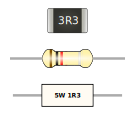
\includegraphics[width=0.4\textwidth]{ResistorPackages}
\caption{Common Resistor Packages}
\end{figure}

As can be seen from the middle resistor image, bands are frequently used on through hole resistors, so that from any angle their resistance can be read. Below is a reference guide for this, which is worthwhile remembering. Although, there are plenty of online calculators, where you can enter the bands to see the resistance. Alternatively, a multimeter should provide a quick and accurate resistance measurement, which is discussed later in the document.



\Examples{Example circuits etc}

This is a basic circuit, with wires, a \gls{rstr} and a battery, to demonstrate V=IR. \href{https://tinyurl.com/27gj49kj}{Link}

In the specific example, we have a \gls{rstr} of 1 Ohms and a \gls{vltg} of 5V. Therefore, using $V=IR$, we can rearrange to find a \gls{crnt} of $I = 5/1 = 5A$. Then we can find a power of $P = IV = 5*5 = 25W$. The simulation shows each of these. Feel free to play around with it and alter values. Instructions for using the simulation program are found (here).

There aren't many example circuits using the above knowledge alone. One example would be a heater project. Given you know the available input \gls{vltg}, and the needed thermal load, you can calculate the required heating element \gls{rstnc}.

There may be the case where a constant heat power output is required. A resistor is purely resistive, so all the electrical power it uses should be dissipated as heat. Lets say there is a supply of 240V (to simply represent mains voltage), and a 2000W supply of heat is required (of a similar magnitude to an oven). Therefore, using $V=IR$ and $P=IV$. Starting with $P=IV$, we can find a current of the below:
\[I=\frac{P}{V}, I=\frac{2000}{240}, I=\frac{25}{3}A\]
We can now use this in:
\[V=IR, R=\frac{V}{I}, R=\frac{240}{\frac{25}{3}}, R=28.8\ohm\]
In reality, most heater systems will have a control loop, with a focus to achieve and then sustain a given temperature, so there would be an element of sensing and turning the heater on and off, which we will get to later in the document.

\Quiz{Quiz}

1. True or false, power draw is always constant for a given \gls{rstr}, whatever circuit it is in?

2. True or false, \gls{rstr}s are available in a wide range of \gls{rstnc} values, but multiple can be used together to achieve more specific values?

3. True or false, \gls{rstr}s convert electrical energy to thermal energy?

\vspace*{1\baselineskip}

\subsection{Potentiometers}

A \gls{ptmtr} is a variable \gls{rstr} acting as a \gls{ptldvdr}, using a dial to alter its output \gls{rstnc}. There are many cases where this is helpful, like altering speaker volume, or where \gls{vltg} needs aren't clear or certain. They typically have 3 pins, for the input, ground and output. The input and output together act as a \gls{rstr}, with a value depending on how far the dial is turned.

\gls{dgtl} \gls{ptmtr}s are an example of an integrated circuit, which are programmed to act as a set \gls{rstnc}, using steps, meaning the same resolution isn't usually attainable.

\begin{figure}[H]
\centering
\includegraphics[width=0.4\textwidth]{Potentiometer1}
\caption{Potentiometer on the left, Variable resistor on the right}
\end{figure}

\begin{figure}[H]
\centering
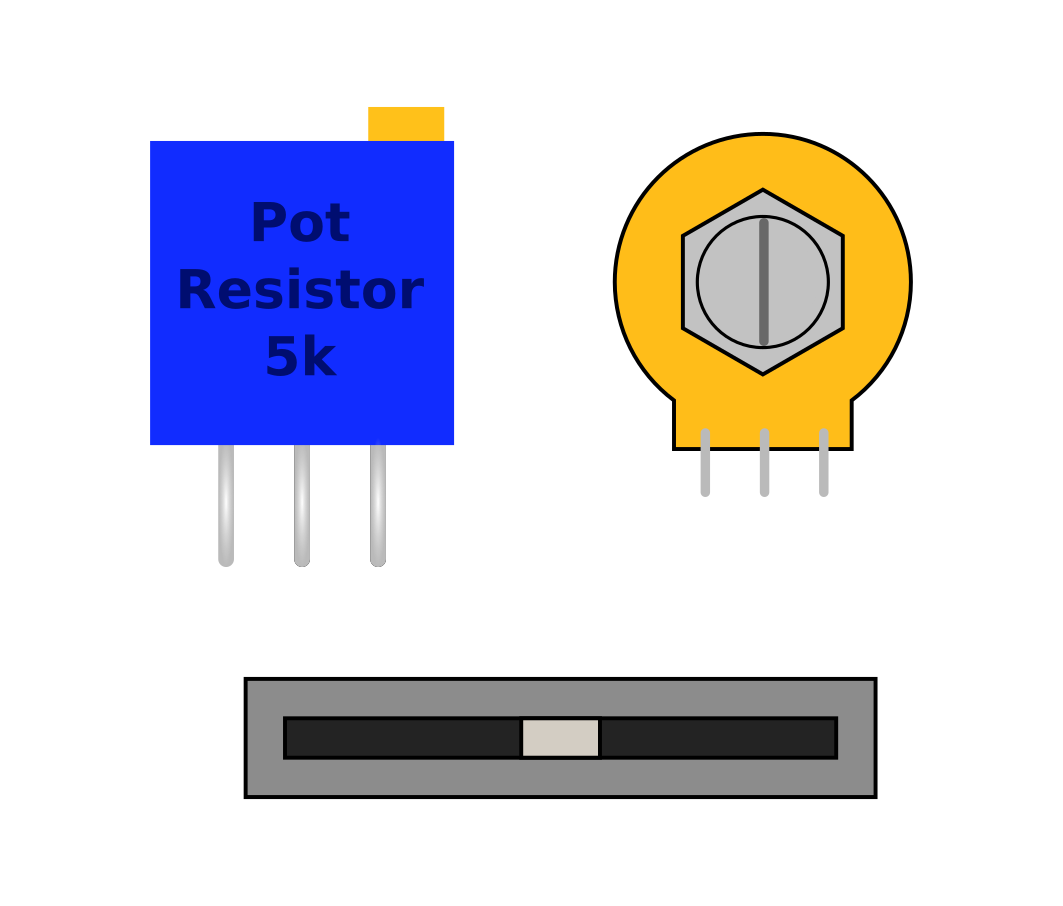
\includegraphics[width=0.4\textwidth]{PotentiometerPackages}
\caption{Common Potentiometer Packages}
\end{figure}

\vspace*{1\baselineskip}

\subsection{Series and Parallel}

You can wire a circuit with \gls{prl} and \gls{srs} elements. A \gls{srs} circuit has a single loop, with components connected one after another, sharing a single \gls{vltg}. A \gls{prl} circuit can have more than one loop branching out. Each loop has a \gls{vltg} equivalent to the input, with the \gls{crnt} split between them, based on their \gls{rstnc}.

Therefore, the \gls{vltg} in a \gls{srs} loop will be distributed based on the \gls{vltg} ratios. For example, there is a 10$\ohm$ and 5$\ohm$ \gls{rstr}, with a 9V supply. There would be a \gls{vltg} drop of 6V through the 10$\ohm$ \gls{rstr} and a 3V drop through the 5$\ohm$ \gls{rstr}. With a total \gls{rstnc} of 15$\ohm$, we can calculate the \gls{crnt} to be $V=IR$, $I=\frac{V}{R}$, $I=\frac{9}{15}=0.6A$.

\begin{figure}[H]
\centering
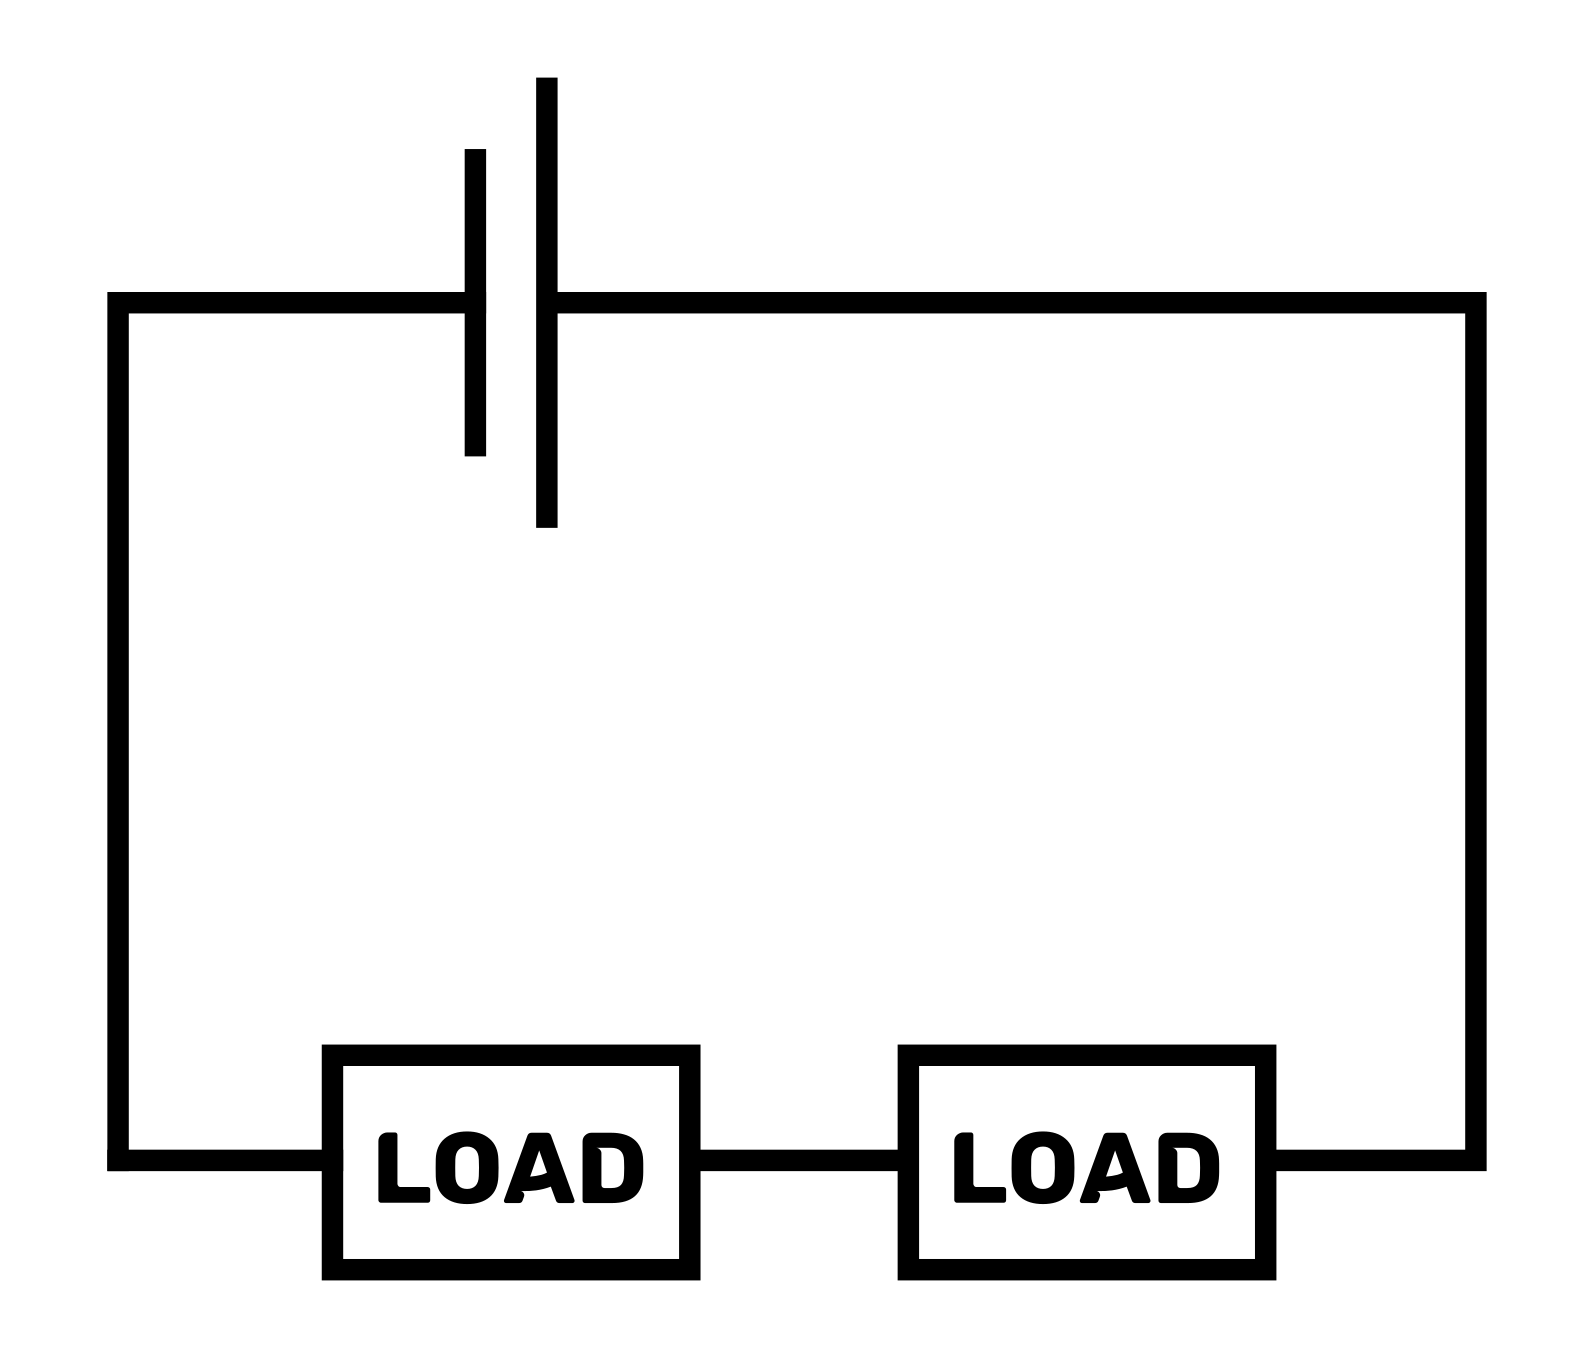
\includegraphics[width=0.4\textwidth]{series1}
\caption{Series base example circuit}
\end{figure}

\begin{figure}[H]
\centering
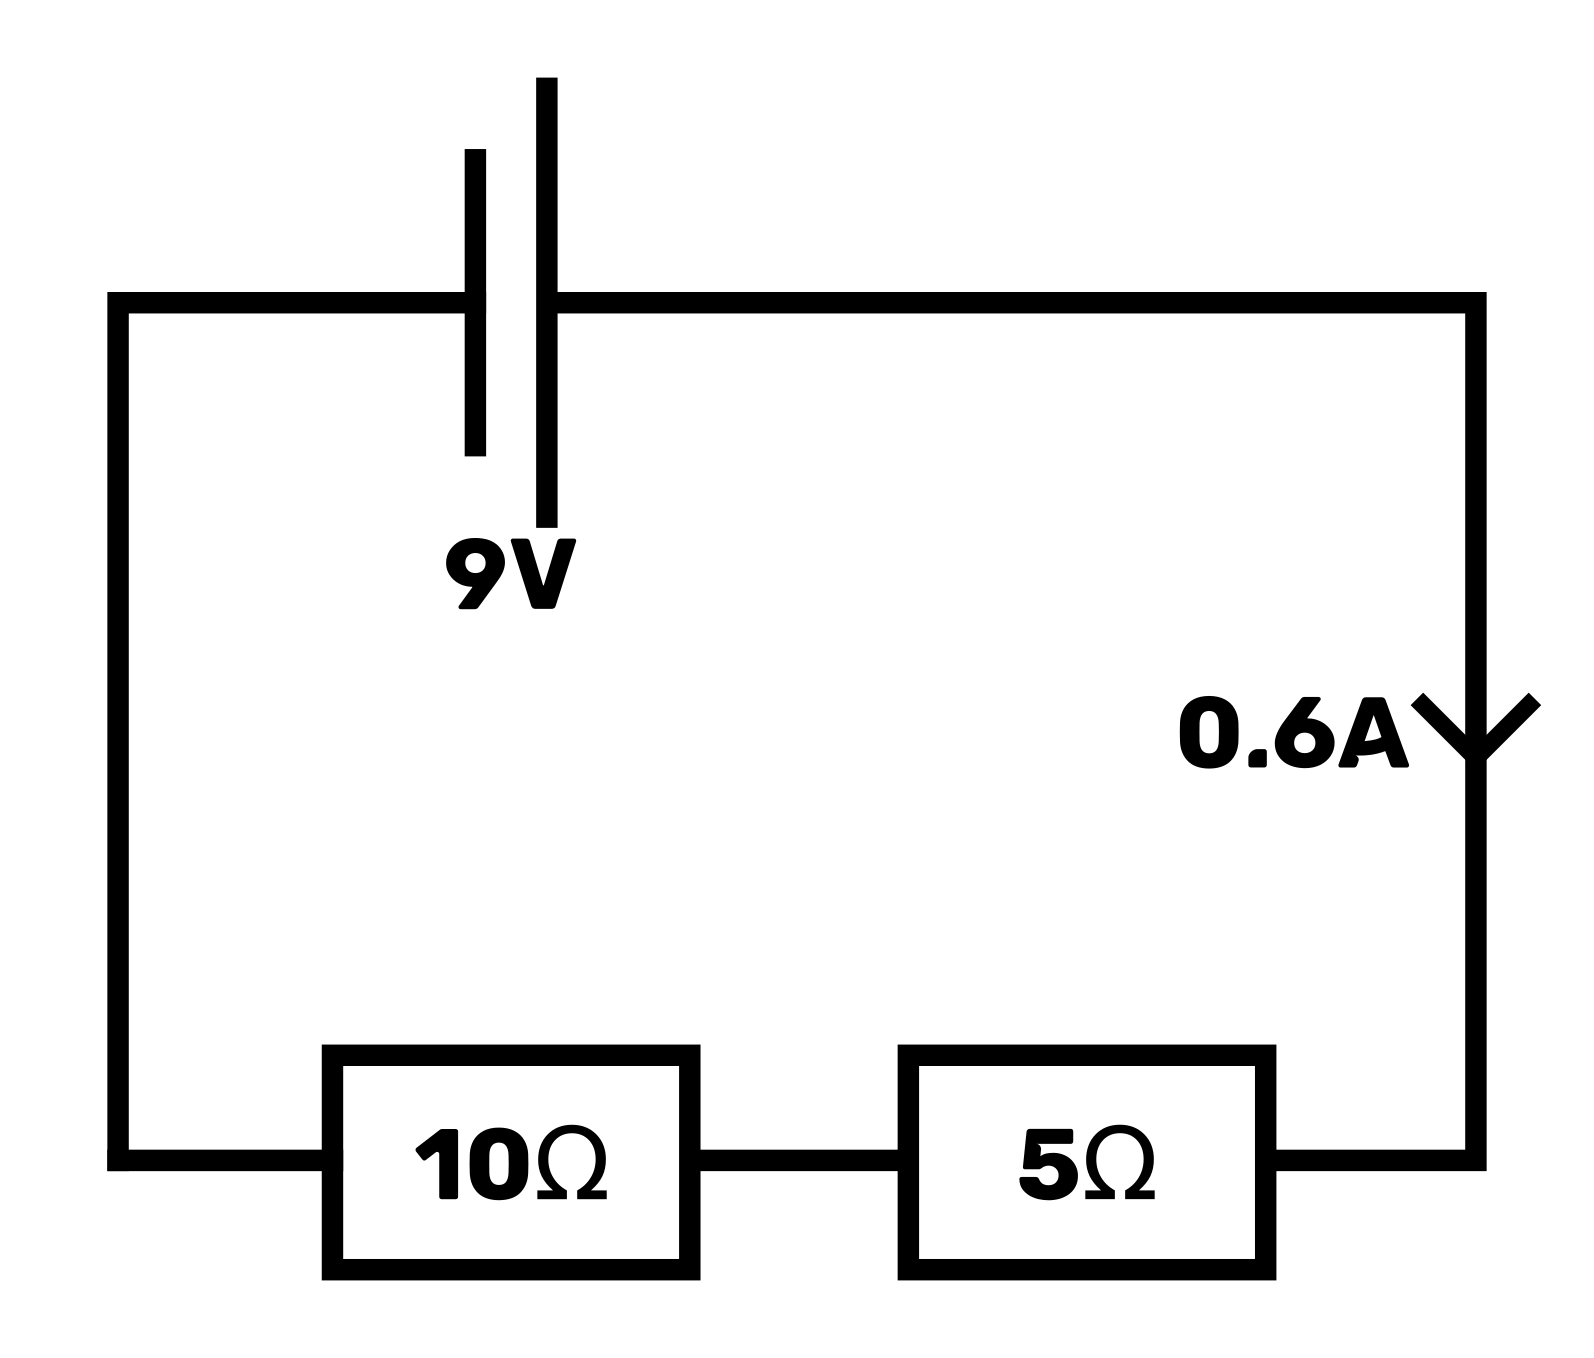
\includegraphics[width=0.4\textwidth]{series2}
\caption{Series example circuit 1}
\end{figure}

A \gls{prl} circuit has equal \gls{vltg} across each path, with the \gls{crnt} being split. Because of this, \gls{rstr}s in \gls{prl} have a total \gls{rstnc} lower than the lowest \gls{rstnc} path.
We can calculate this using the below equation:
\[\frac{1}{R_{total}} = \frac{1}{R_1} + \frac{1}{R_2} + \frac{1}{R_3} + \cdots\]

\begin{figure}[H]
\centering
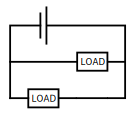
\includegraphics[width=0.4\textwidth]{parallel1}
\caption{Parallel base example circuit}
\end{figure}

\begin{figure}[H]
\centering
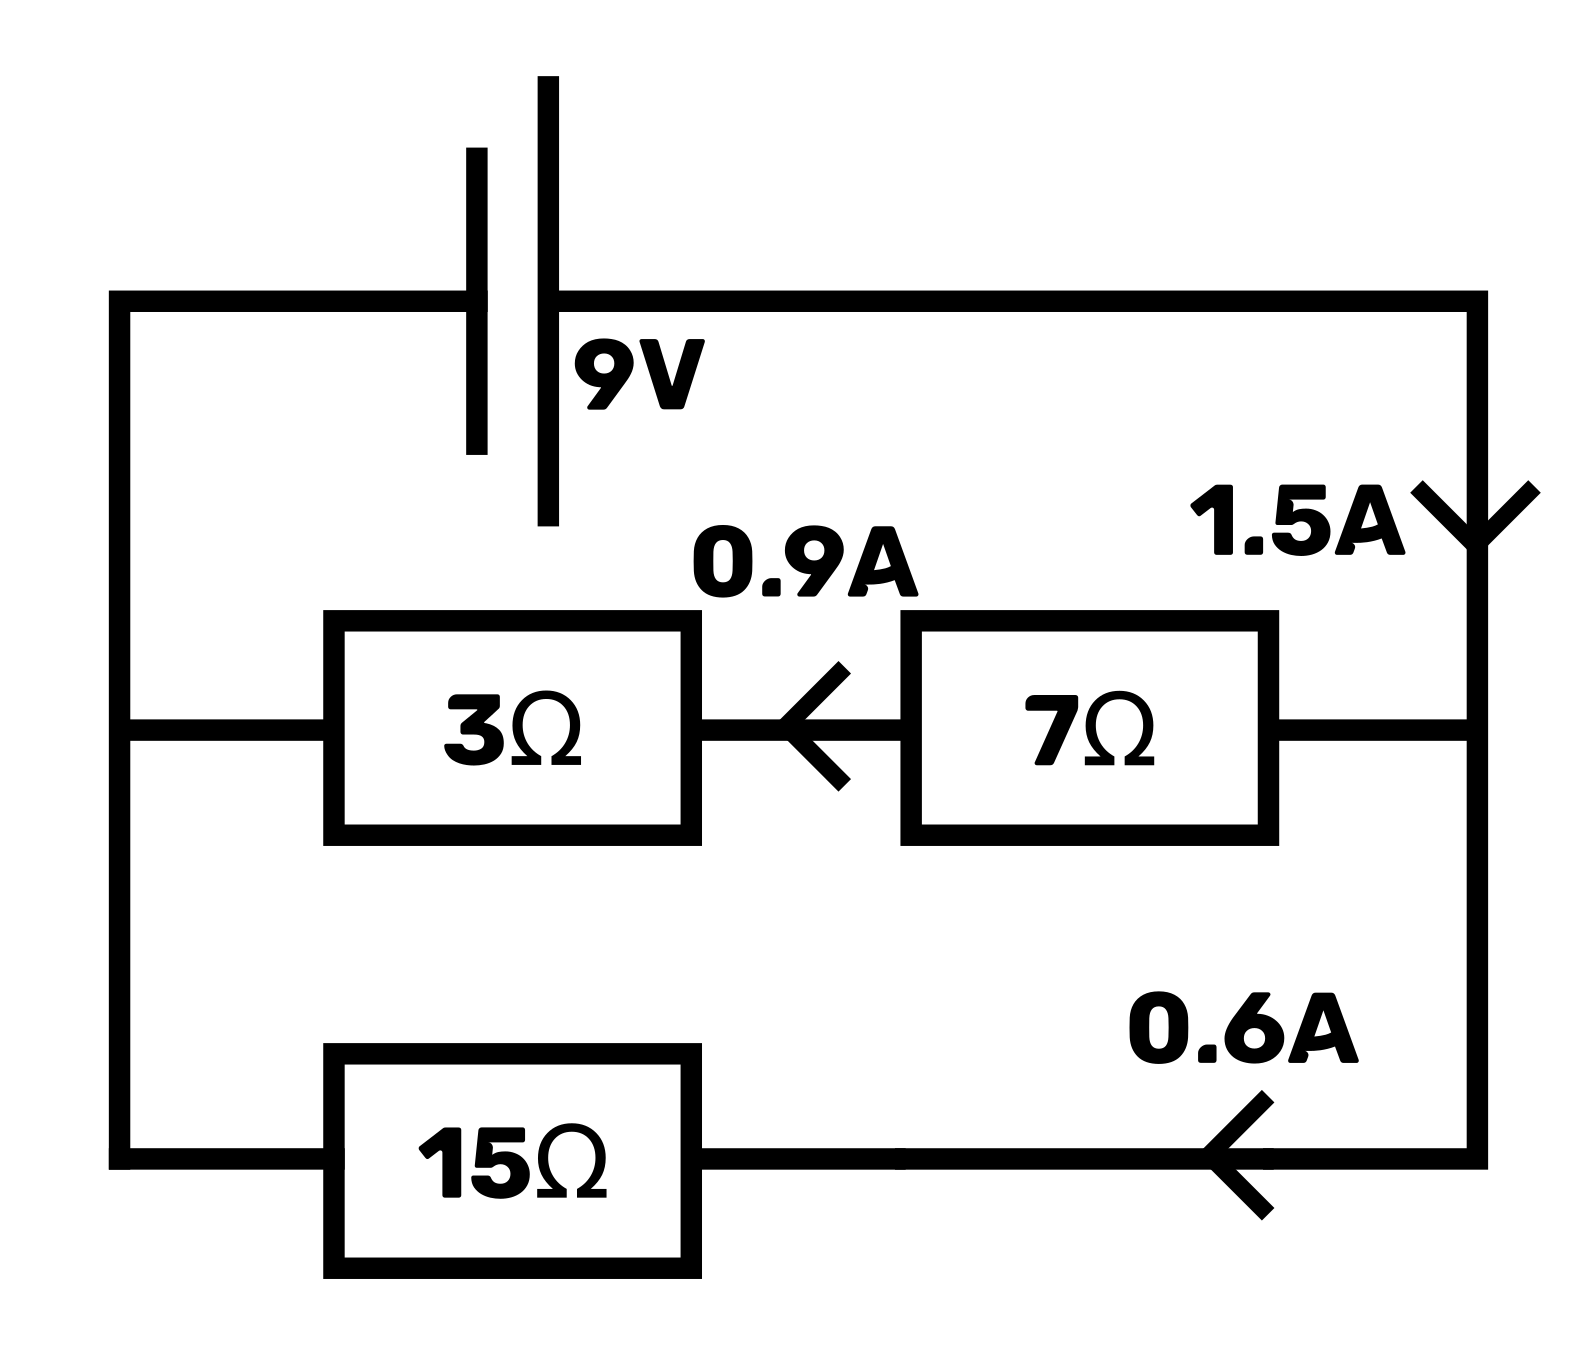
\includegraphics[width=0.4\textwidth]{parallel2}
\caption{Parallel example circuit 1}
\end{figure}

Therefore, an example with the following circuit with 2 \gls{rstr}s of 3$\ohm$ and 7$\ohm$, in \gls{prl} with a single \gls{rstr} of 15$\ohm$. You first add the \gls{srs} \gls{rstr}s, therefore an equivalent resistor $R_1$ is 10$\ohm$ and $R_2$ is 15$\ohm$. Putting it into the equation gives us the below:
\[\frac{1}{R_{total}} = \frac{1}{10} + \frac{1}{15}\]
\[\frac{1}{R_{total}} = \frac{1}{6}\]
\[R_{total} = 6\ohm\]

If we were to think again of the mail network analogy, a series circuit has the mailpeople take multiple stops on their journey, handing a certain amount of letters to each, depending on their need/\gls{rstnc}. With a parallel circuit, some mailpeople will focus on different paths, so will still have the same total parcels for their path (the voltage stays the same for each path). The current decreases, since the mailpeople split to go down different routes.

\Examples{Example circuits etc}

A basic example would be a basic circuit to "divide" a \gls{vltg}. \href{https://tinyurl.com/27sybjry}{Link}

\Quiz{Quiz}

1. Which of the following statements are true?

a) \gls{crnt} is equal down each path from a junction.

b) \gls{crnt} splits at a path junction, based on each paths \gls{rstnc}.

c) \gls{vltg} is equal down each path from a junction.

d) \gls{vltg} splits at a path junction, based on each path's \gls{rstnc}.

2. What is the \gls{vltg} drop of each component? Also, calculate the power of the circuit.

\begin{figure}[H]
\centering
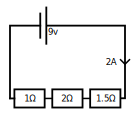
\includegraphics[width=0.4\textwidth]{series3}
\caption{Series example circuit 2}
\end{figure}

3. What is the equivalent \gls{rstnc} of a 20$\ohm$, 100$\ohm$ and 42$\ohm$ component, all in \gls{prl}?

4. True or false, the power draw through two  20 $\ohm$ \gls{rstr}s is higher than through a single 10 ohm \gls{rstr}?

\vspace*{1\baselineskip}

\subsection{Potential Dividers}

\gls{ptldvdr}s use knowledge of both \gls{prl} circuits and \gls{rstnc}. As the name suggests, they help to divide \gls{vltg} potential based on the use of \gls{srs} \gls{rstr}s. As stated before, within a \gls{srs} path, the \gls{vltg} will be divided between the components based on their \gls{rstnc}.

\begin{figure}[H]
\centering
\includegraphics[width=0.4\textwidth]{PotentialDivider}
\caption{Potential Divider base example circuit}
\end{figure}

Therefore, if there was an input \gls{vltg} of 5V, and R1 has a \gls{rstnc} of 10$\ohm$ and R2 has a \gls{rstnc} of 3$\ohm$, then the \gls{vltg} seen through the \gls{ptldvdr}'s output is the below:
\[V_{out}=\frac{(R_1+R_2)-R_2}{R_1+R_2}*V_{in} = \frac{10}{13}*5 = \frac{50}{13}V\]

\vspace*{1\baselineskip}

\subsection{AC vs DC}

\gls{atngcrt} stands for alternating \gls{crnt}, whereas \gls{drtcrt} stands for direct \gls{crnt}. This is shown on a graph with the direction of flow on one axis and magnitude of \gls{vltg} on the other. \gls{drtcrt} has a constant magnitude and direction of flow. This compares to a sinusoidal \gls{vltg} magnitude with \gls{atngcrt}, where the flow of \gls{crnt} varies in direction. \gls{atngcrt} is typically given as an \gls{rms} \gls{vltg} and a frequency. The frequency is the number of \gls{prd}s that happen per second, typically given in Hz, where the \gls{vltg} is an average value, taking the root mean square. Root mean square (\gls{rms}) represents the \gls{drtcrt} \gls{vltg} that has the same power/ heating effect as the \gls{atngcrt} circuit. This is seen with power from the \gls{grd}, with \gls{rms} \gls{vltg}s of 230V and frequency of 50Hz in the UK.
Being in \gls{atngcrt} allows for high \gls{vltg} conversion through long distance cables using \gls{trnfmr}s, to reduce thermal losses due to heat from high \gls{crnt}.
This is particularly important, as using $P=I^2R$, we can see that power compared to current is a quadratic, so with a fixed cable resistance, the higher the current, the larger the increase of heat loss.

\begin{figure}[H]
\centering
\includegraphics[width=0.4\textwidth]{acsource1}
\caption{AC Source circuit icon}
\end{figure}

\begin{figure}[H]
\centering
\includegraphics[width=0.4\textwidth]{dcsource1}
\caption{DC Source circuit icon}
\end{figure}

\begin{figure}[H]
\centering
\includegraphics[width=0.4\textwidth]{acwave}
\caption{AC Wave example graph}
\end{figure}

\begin{figure}[H]
\centering
\includegraphics[width=0.4\textwidth]{dcwave}
\caption{DC Wave example graph}
\end{figure}

\gls{dgtl} electronics are within the \gls{drtcrt} realm, but many devices still require \gls{atngcrt}. It is the standard for energy generation and for how it is sent across the \gls{grd}. \gls{atngcrt} is widely used for \gls{mtr}s, and where large \gls{vltg} transformations are required, such as microwaves. \gls{smicdtr} electronics primarily work within \gls{drtcrt}.

The course will touch upon ways to convert between \gls{atngcrt}-\gls{drtcrt} and the benefits of each for different applications.

\Quiz{Quiz}

1. What is the frequency of \gls{atngcrt} Electricity from the \gls{grd} in the UK?

2. What does \gls{rms} stand for?

3. Why is \gls{atngcrt} used within the \gls{grd}?

\vspace*{1\baselineskip}

\subsection{Capacitors}

\Theory{What are \gls{cptr}s?}

\gls{cptr}s are another key component. They store energy as Electric Potential, with their \gls{vltg} increasing towards the input \gls{vltg}, as they charge. Therefore, the charge and discharge curve is nonlinear, more similar to a natural log curve.

\begin{figure}[H]
\centering
\includegraphics[width=0.4\textwidth]{capacitorcharge}
\caption{Capacitor charge voltage graph}
\end{figure}

\begin{figure}[H]
\centering
\includegraphics[width=0.4\textwidth]{capacitordischarge}
\caption{Capacitor discharge voltage graph}
\end{figure}

The unit for \gls{cptnc} is \gls{frd}, with typical values depending on \gls{cptr} type, but usually in the uF units or below.

A range of physics based equations will be touched upon now.

\gls{cptr}s have a charge relating to their input \gls{vltg} with the following basic equation: $q = CV$.  C is \gls{cptnc}, q is charge, and V is \gls{vltg}. There is also the formula for energy stored within a \gls{cptr}, with the following equation: $E = 1/2*C*V^2$, where E is energy in \gls{jls}.

A \gls{rstr} is usually placed in \gls{srs} with a \gls{cptr} to limit the \gls{cptr} inlet \gls{crnt}. As it charges, the ratio between its \gls{vltg} and the supply \gls{vltg} decreases, along with the charge \gls{crnt}, in a curve of reverse direction to the \gls{vltg}.

\begin{figure}[H]
\centering
\includegraphics[width=0.4\textwidth]{capacitorchargecurrent}
\caption{Capacitor charge current graph}
\end{figure}

\begin{figure}[H]
\centering
\includegraphics[width=0.4\textwidth]{capacitordischargecurrent}
\caption{Capacitor discharge current graph}
\end{figure}

One of the built-in simulation circuits from Falstad is helpful for showcasing the charge and discharge characteristics of a \gls{cptr}, by flicking a switch. \href{https://tinyurl.com/2erbz4jy}{Link}

You should be aware of what happens with \gls{srs} and \gls{prl} \gls{cptr}s. The \gls{cptnc} of \gls{cptr}s add when in \gls{prl}, where in \gls{srs}, it is like \gls{rstr}s in \gls{prl}. You can think of it having inverse rules to the \gls{rstr}. Therefore, \gls{cptr}s are often used in \gls{prl} but less so in \gls{srs}, unless a higher \gls{vltg} is required than their individual rated value. Shown by the equations below:

\gls{srs} \gls{cptr}s- \[C_{total} = \frac{1}{\frac{1}{C_1}+\frac{1}{C_2}+\cdots}\]

\gls{prl} \gls{cptr}s- \[C_{total} = C_1+C_2+\cdots\]

\begin{figure}[H]
\centering
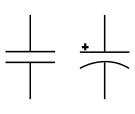
\includegraphics[width=0.4\textwidth]{capacitor1}
\caption{Bipolar capacitor on left, Polar capacitor on right}
\end{figure}

\begin{figure}[H]
\centering
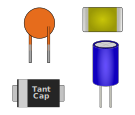
\includegraphics[width=0.4\textwidth]{CapacitorPackages}
\caption{Common Capacitor Packages}
\end{figure}

\Examples{Example circuits etc}

\Quiz{Quiz}

1. How do \gls{cptr}s store energy?

a) In the magnetic field

b) In the electric field

c) As thermal energy

d) They do not store energy

2. True or false, a \gls{rstr} is typically used in \gls{srs} with a \gls{cptr} to limit \gls{crnt} flow through the \gls{cptr}.

3. True or false, 1 \gls{frd} \gls{cptr}s are commonly available.

4. Design a circuit for charging a \gls{cptr} at a maximum \gls{crnt} of 1A, assuming a source \gls{vltg} of 3V.

\vspace*{1\baselineskip}

\subsection{Inductors}

\Theory{What are \gls{indctr}s?}

\gls{indctr}s are another key passive energy storage component. These store energy within the magnetic field, and have a range of uses, often in power electronics.

The unit for \gls{idtnc} (L) is \gls{hnry}, with typical values depending on \gls{indctr} type, but usually in the uH or mH units or below.

A range of physics based equations are used to show \gls{idtnc}.

There is the following basic equation: $L = \frac{\Phi(i)}{i}$. There is also the energy formula for calculating the energy stored within an \gls{indctr}, with the following basic equation: $E = 1/2*L*I^2$.

It is also useful to be aware of the rules for \gls{srs} and \gls{prl} \gls{indctr}s. It is like the rules for \gls{rstr}s, although this time being \gls{idtnc}.

\gls{srs} \gls{indctr}s- \[L_{total} = L_1 + L_2 + \cdots\]

\gls{prl} \gls{indctr}s- \[L_{total} = \frac{1}{\frac{1}{L_1}+\frac{1}{L_2}}\]

\begin{figure}[H]
\centering
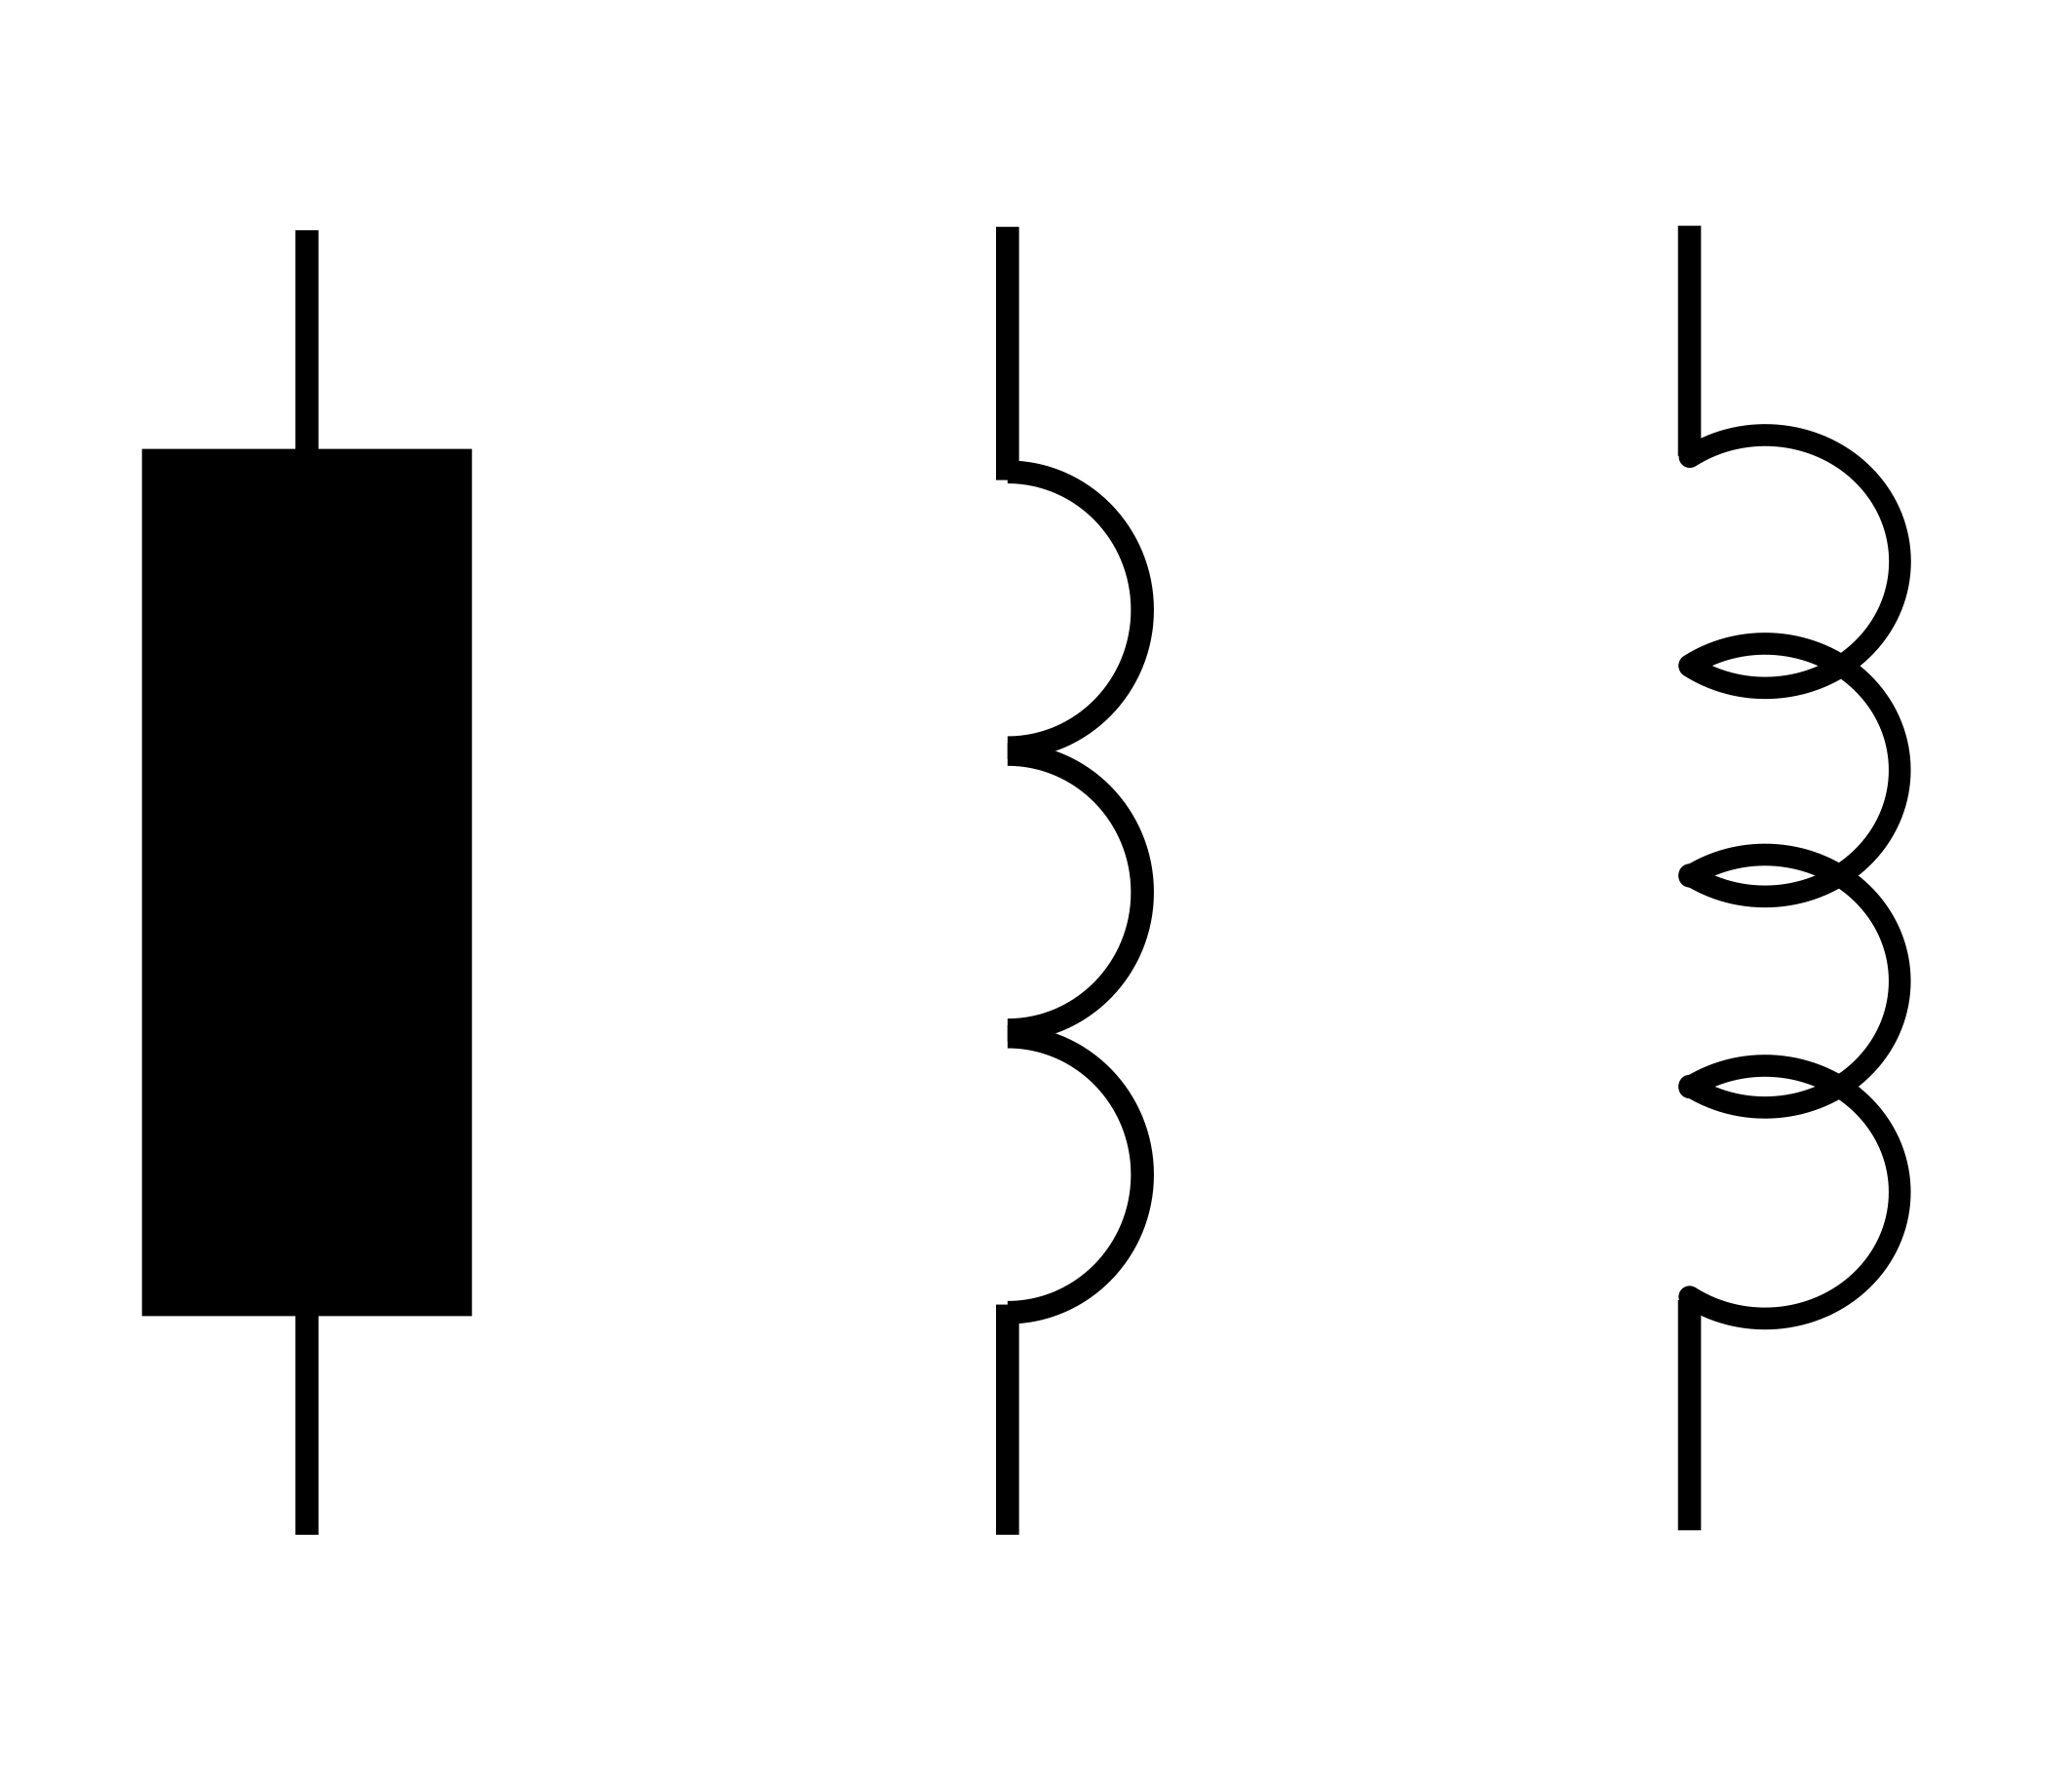
\includegraphics[width=0.4\textwidth]{inductor1}
\caption{Inductor representations}
\end{figure}

\begin{figure}[H]
\centering
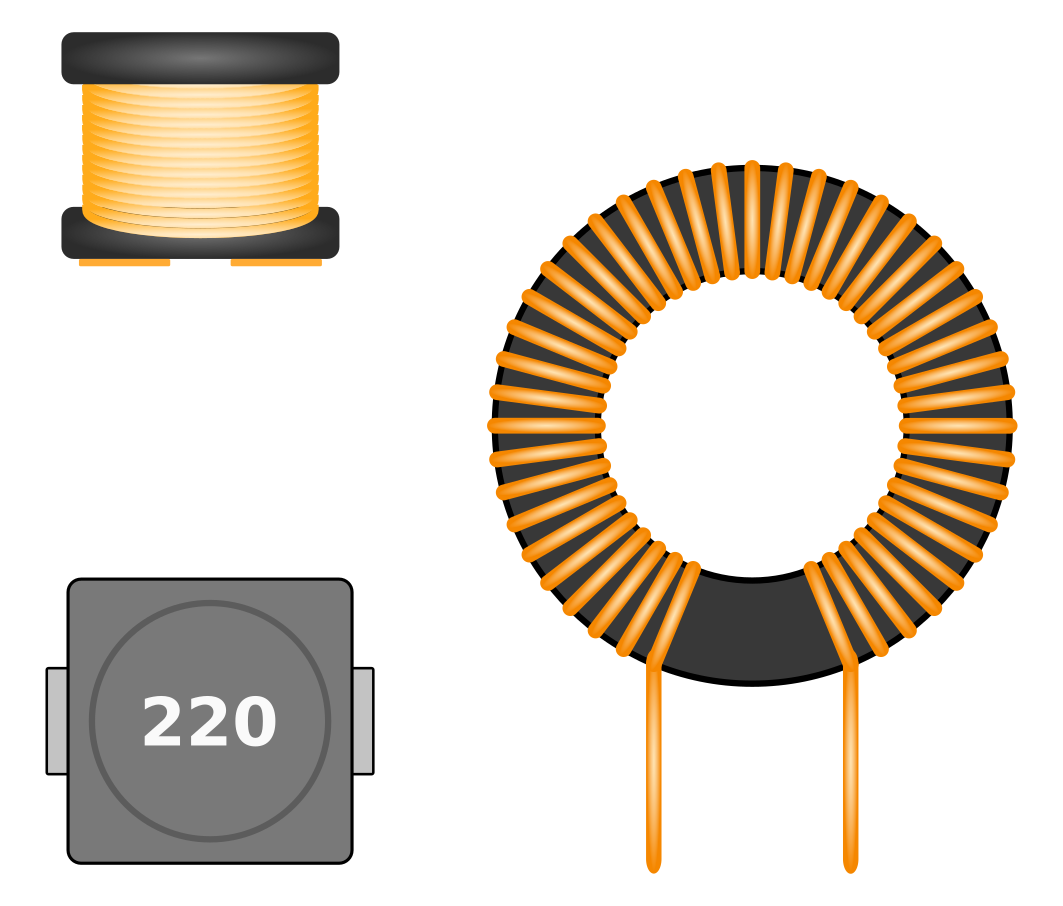
\includegraphics[width=0.4\textwidth]{InductorPackages}
\caption{Common Inductor Packages}
\end{figure}

One of the built-in simulation circuits from Falstad is helpful for showcasing the charge and discharge characteristics of an \gls{indctr}, by flicking a switch. \href{https://tinyurl.com/2brgydk6}{Link}

\Examples{Example circuits etc}

\Quiz{Quiz}

1. What units is \gls{idtnc} given in?

\vspace*{1\baselineskip}

\subsection{Diodes}

\gls{diod}s are widely used in electronics. The basic principle of a \gls{diod} is a device/component which limits how \gls{crnt} can flow within a circuit, such as restricting \gls{crnt} flow to one direction.
This makes them beneficial for a range of circuits, such as protection circuits, preventing unwanted reverse \gls{crnt} flow, which could damage other components or cause unwanted side effects.
They are a simpler examples of a \gls{smicdtr}, where usually silicon is \gls{dpd} with other atoms to cause a surplus or shortage of electrons, changing the polarity of elements of the material, affecting how \gls{crnt} flows through the \gls{diod}.

There are also Light Emitting \gls{diod}s (\gls{led}s), which work through similar principles, but emit light of a certain spectrum depending upon \gls{led} selection. There is a \gls{vltg} drop associated with this, but with considerably lower heat output, compared to filament bulbs, which heat filament until it glows. Therefore

There is a common formula for calculating the \gls{rstr} needed for an \gls{led}, given you know its \gls{vltg} drop and the \gls{crnt} it runs at. This is the following:
\[R = \frac{V_s - V_f}{I_f}\]
Where $V_s$ is the supply \gls{vltg}, $V_f$ is the forward \gls{vltg} (\gls{vltg} drop of the \gls{led}) and $I_f$ is the forward \gls{crnt}.

Different colour \gls{led}s work at different \gls{vltg}s, so \gls{rstr}s are commonly used to drop the input \gls{vltg} to a level suitable for the \gls{led}. The \gls{led}s also help to limit \gls{crnt} through the \gls{led}. This \gls{vltg} usually is between 1.8-3.3v, and is because of how the \gls{smicdtr} is \gls{dpd}, as different dopants will cause different \gls{wvlgt}s of light to be emitted.

It is important to consider that \gls{diod}s have an inherent \gls{vltg} drop, so this needs to be considered, especially when using them with low-\gls{vltg} circuits, as a typical \gls{diod} can have \gls{vltg} drops between around 0.4-0.7v.

There are many subcategories of \gls{diod}s. The most common type mentioned above is known as a junction \gls{diod}. \gls{znr} \gls{diod}s allow reverse \gls{crnt} after a certain threshold \gls{vltg} is met. A \gls{shtky} \gls{diod} has low \gls{vltg} drop and fast switching. There are also \gls{diac}s and \gls{tric}s for \gls{atngcrt}, allowing some \gls{crnt} flow in both directions.

\begin{figure}[H]
\centering
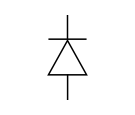
\includegraphics[width=0.4\textwidth]{diode1}
\caption{Diode representation}
\end{figure}

\begin{figure}[H]
\centering
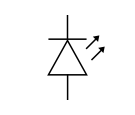
\includegraphics[width=0.4\textwidth]{diode2}
\caption{Light Emitting Diode representation}
\end{figure}

\begin{figure}[H]
\centering
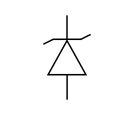
\includegraphics[width=0.4\textwidth]{diode3}
\caption{Zener Diode representation}
\end{figure}

\begin{figure}[H]
\centering
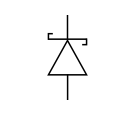
\includegraphics[width=0.4\textwidth]{diode4}
\caption{Schottky Diode representation}
\end{figure}

\begin{figure}[H]
\centering
\includegraphics[width=0.4\textwidth]{diodepackages}
\caption{Common Diode Packages}
\end{figure}

\begin{figure}[H]
\centering
\includegraphics[width=0.4\textwidth]{ledpackages}
\caption{Common LED Packages}
\end{figure}

\Quiz{Quiz}

1. Name 4 examples of \gls{diod}s, and what they do?

2. True or false, \gls{diod}s always restrict \gls{crnt} flow to one direction?

3. You are building a low \gls{vltg} circuit, and need to limit \gls{crnt} flow to one direction, but with as low losses as possible. What \gls{diod} would you recommend?

4. True or false, \gls{led}s can be found in a range of colours, each with differing \gls{vltg} drops?

5. Design a \gls{led} circuit, with an input \gls{vltg} of 3V and the \gls{led} has a \gls{vltg} drop of 1.8V running at its recommended \gls{crnt} of 25mA. What is the total power consumption of this circuit?

\vspace*{1\baselineskip}

\subsection{Transformers}

\Theory{What are \gls{trnfmr}s?}

\gls{trnfmr}s use the fact that a \gls{crnt} carrying coil of wire will generate a magnetic field, which induces a \gls{crnt} in a coil to allow for \gls{vltg}/ \gls{crnt} conversion. Think of it as two \gls{indctr}s, \gls{cupld} through a single \gls{core}. This is typically a \gls{frtc} \gls{core} to provide a magnetic path to reduce losses. These are often laminated to limit eddy \gls{crnt}s, which are loops of \gls{crnt} within the \gls{core}, induced from the magnetic field. \gls{lmntn} increases the \gls{core} \gls{rstnc}, reducing the eddy \gls{crnt}.

A lot of \gls{trnfmr} design is out of the courses scope. We will assume that the \gls{trnfmr} is ideal, although in reality, there are losses, leading to efficiencies of upwards of 95\%. This depends on how well suited a \gls{trnfmr} is for a design.

Due to \gls{crnt} only being induced under a changing magnetic field, \gls{trnfmr}s only work with an \gls{atngcrt} input.

This is the basic set of equations for \gls{trnfmr}s.

\[\frac{V_p}{V_s} = \frac{I_s}{I_p} = \frac{N_p}{N_s}\]

Where p represents the input/ primary coil and s represents the output/ secondary coil. V represents \gls{vltg}, I represents \gls{crnt} and N represents the number of turns/ coils.

There is an inverse relationship between \gls{vltg} and \gls{crnt} when there are different coil turns.

There are 1:1 \gls{trnfmr}s, where no \gls{vltg} or \gls{crnt} conversion takes place, but it isolates the input from the output, so is a safety feature often used in products. These are known as isolation \gls{trnfmr}s.

\begin{figure}[H]
\centering
\includegraphics[width=0.4\textwidth]{Transformer1}
\caption{Transformer representation}
\end{figure}

\begin{figure}[H]
\centering
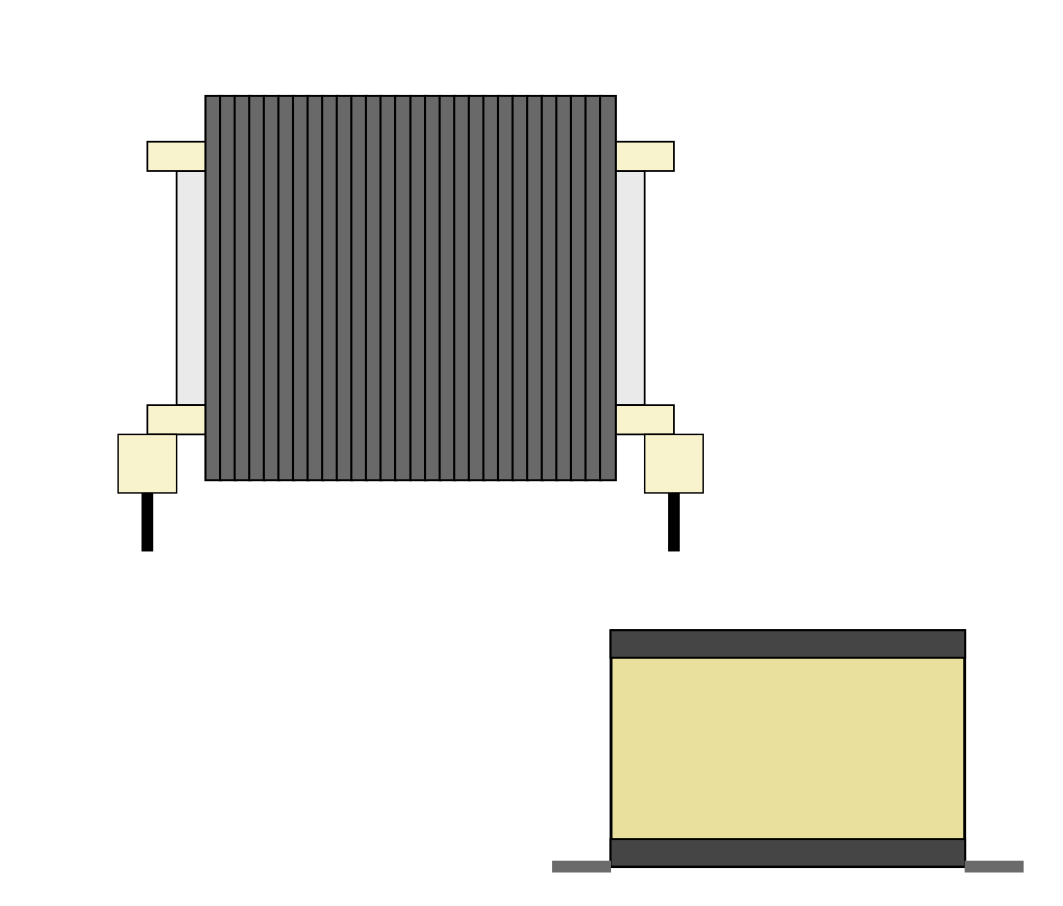
\includegraphics[width=0.4\textwidth]{TransformerPackages}
\caption{Example Transformer Packages}
\end{figure}

\Quiz{Quiz}

1. Why are \gls{trnfmr} coils often laminated?

2. A \gls{trnfmr} with a 240V \gls{rms} input with a peak \gls{crnt} capability of 0.1A, with 100 turns on its primary side, needs to supply a 12V \gls{rms} circuit. How many secondary turns are required, and what is the peak \gls{crnt} that could be supplied to the output circuit?

3. Why are isolation \gls{trnfmr}s used?

\vspace*{1\baselineskip}

\subsection{Analogue vs Digital}

It is important to be aware of differences between \gls{anlge} and \gls{dgtl}. \gls{anlge} refers to a wave, with the fundamental characteristics of \gls{wvlgt}, frequency and magnitude. This value can vary considerably within a \gls{prd}, which is particularly useful for some applications.

On the contrary, \gls{dgtl} is represented with either 1 or 0 (off or on). As already touched upon, the entire field of modern \gls{dgtl} electronics is based around \gls{smicdtr}s, which form switches.

Signals can be sent through both methods, with a range of benefits and negatives. A lot of data can be shown in a single \gls{anlge} signal, although it can be difficult to accurately read. Whereas, \gls{drtcrt} deals with two distinct boundaries, so although many more "pulses" are required to output the same amount of data, it is more reliable and easier to use/ read within logic based processing/ \gls{blnalgbr}, which is touched upon later on in the course.

\gls{snsr}s are often read using \gls{anlge} methods, where there is an induced or dropped \gls{vltg} which can vary in magnitude. This would need to be converted to a \gls{dgtl} value for \gls{micrctrlr} use. A combination of \gls{dgtl} 1/0 can be \gls{bnry}, which means a \gls{vltg} value can be represented as a \gls{bnry} combination of 1s and 0s. An ADC is an IC which does this conversion.

\Quiz{Quiz}

1. For a wire communicating over a long distance, would you recommend that an \gls{anlge} or \gls{dgtl} signal be used?

2. Can equivalent numbers be represented with \gls{anlge} and \gls{dgtl}, along with some processing/ data conversion?

\vspace*{1\baselineskip}

\subsection{Mechanical switches}

Switches are used as input devices, where depending on being open or closed, will allow power transmission or not, by opening or closing a circuit. These can be split into many types, such as typically open switches unless pressed, typically closed switches unless pressed, or those which switch between open and closed when pressed, and switches which you can switch to close several sets of pins/ connections.

This section will quickly talk through a few different switches/ buttons, their names and uses.

There are different switches that fit into different classifications, which will briefly be discussed.

Single Pole Single Throw (SPST) switches are ones which connect or break a connection between two single wires/ points/ terminals.

Single Pole Double Throw has a single input but two outputs which can be switched between.

There is then also Double Pole Single Throw, which is a combination of two SPSTs and Double Pole Double Throw, a combination of two SPDTs.

Now onto the different types of switch. They can mainly be split into several types, being the below:

Push button- A typical button, some of which will stay closed/ pressed until pressed again, when others such as momentary push switches will only be closed as they are pressed.

Slide switches are flicked into set position, which can be two positions or multiple.

Toggle is a slight adaptation of slide switches, flicking a centred switch from one angle to another, otherwise working through similar means.

Rotary switches can twist to connect a pin with a range of other pins depending where it is twisted to.

You may have a range of switches, such as a few slide switches packaged together in \gls{dip} format.

\vspace*{1\baselineskip}

\subsection{Digital switches/ Transistors}

Switches are widely used within electronics and are what led to the field of \gls{dgtl} electronics. \gls{micrctrlr}s may use millions of switches on a single silicon \gls{die}, where discrete switches are mainly used for power electronics.

Switches are important to have control of a circuit. These are discussed in greater depth later, but they usually have an externally triggered \gls{gte}, which closes a circuit. Think of a switch as a tap that allows or restricts water flow. The vast majority of these are \gls{smicdtr} based, due to the low losses involved, although they are limited to \gls{drtcrt} function.

This document quickly talks over the main types in detail, so you can understand why each are used, and to help understand surrounding circuitry.

There are \gls{crnt} controlled switches and \gls{vltg} controlled. \gls{bjt}s are an example of a \gls{crnt} controlled switch, where a flow between the \gls{gte} pin and the emitter allows for a higher \gls{crnt} to flow between the emitter to the collector. There is a \gls{vltg} drop, which can mean losses are fairly significant at lower \gls{vltg}s. They are easy to use in a circuit after calculating values.

\begin{figure}[H]
\centering
\includegraphics[width=0.4\textwidth]{BJT}
\caption{Bipolar Junction Transistor (BJT) representation}
\end{figure}

Then there are \gls{vltg} controlled switches, the main example of this being \gls{msft}s. \gls{crnt} can flow after the \gls{vltg} is higher than a threshold is reached in its \gls{gte}. They are more complex to use, since the \gls{gte} acts as a \gls{cptr}, so has to be charged, so may not function well without a properly considered \gls{gte} charge circuit. Losses are related to the \gls{msft}'s internal \gls{rstnc}, which can get very low, so they are typically fairly efficient.

\begin{figure}[H]
\centering
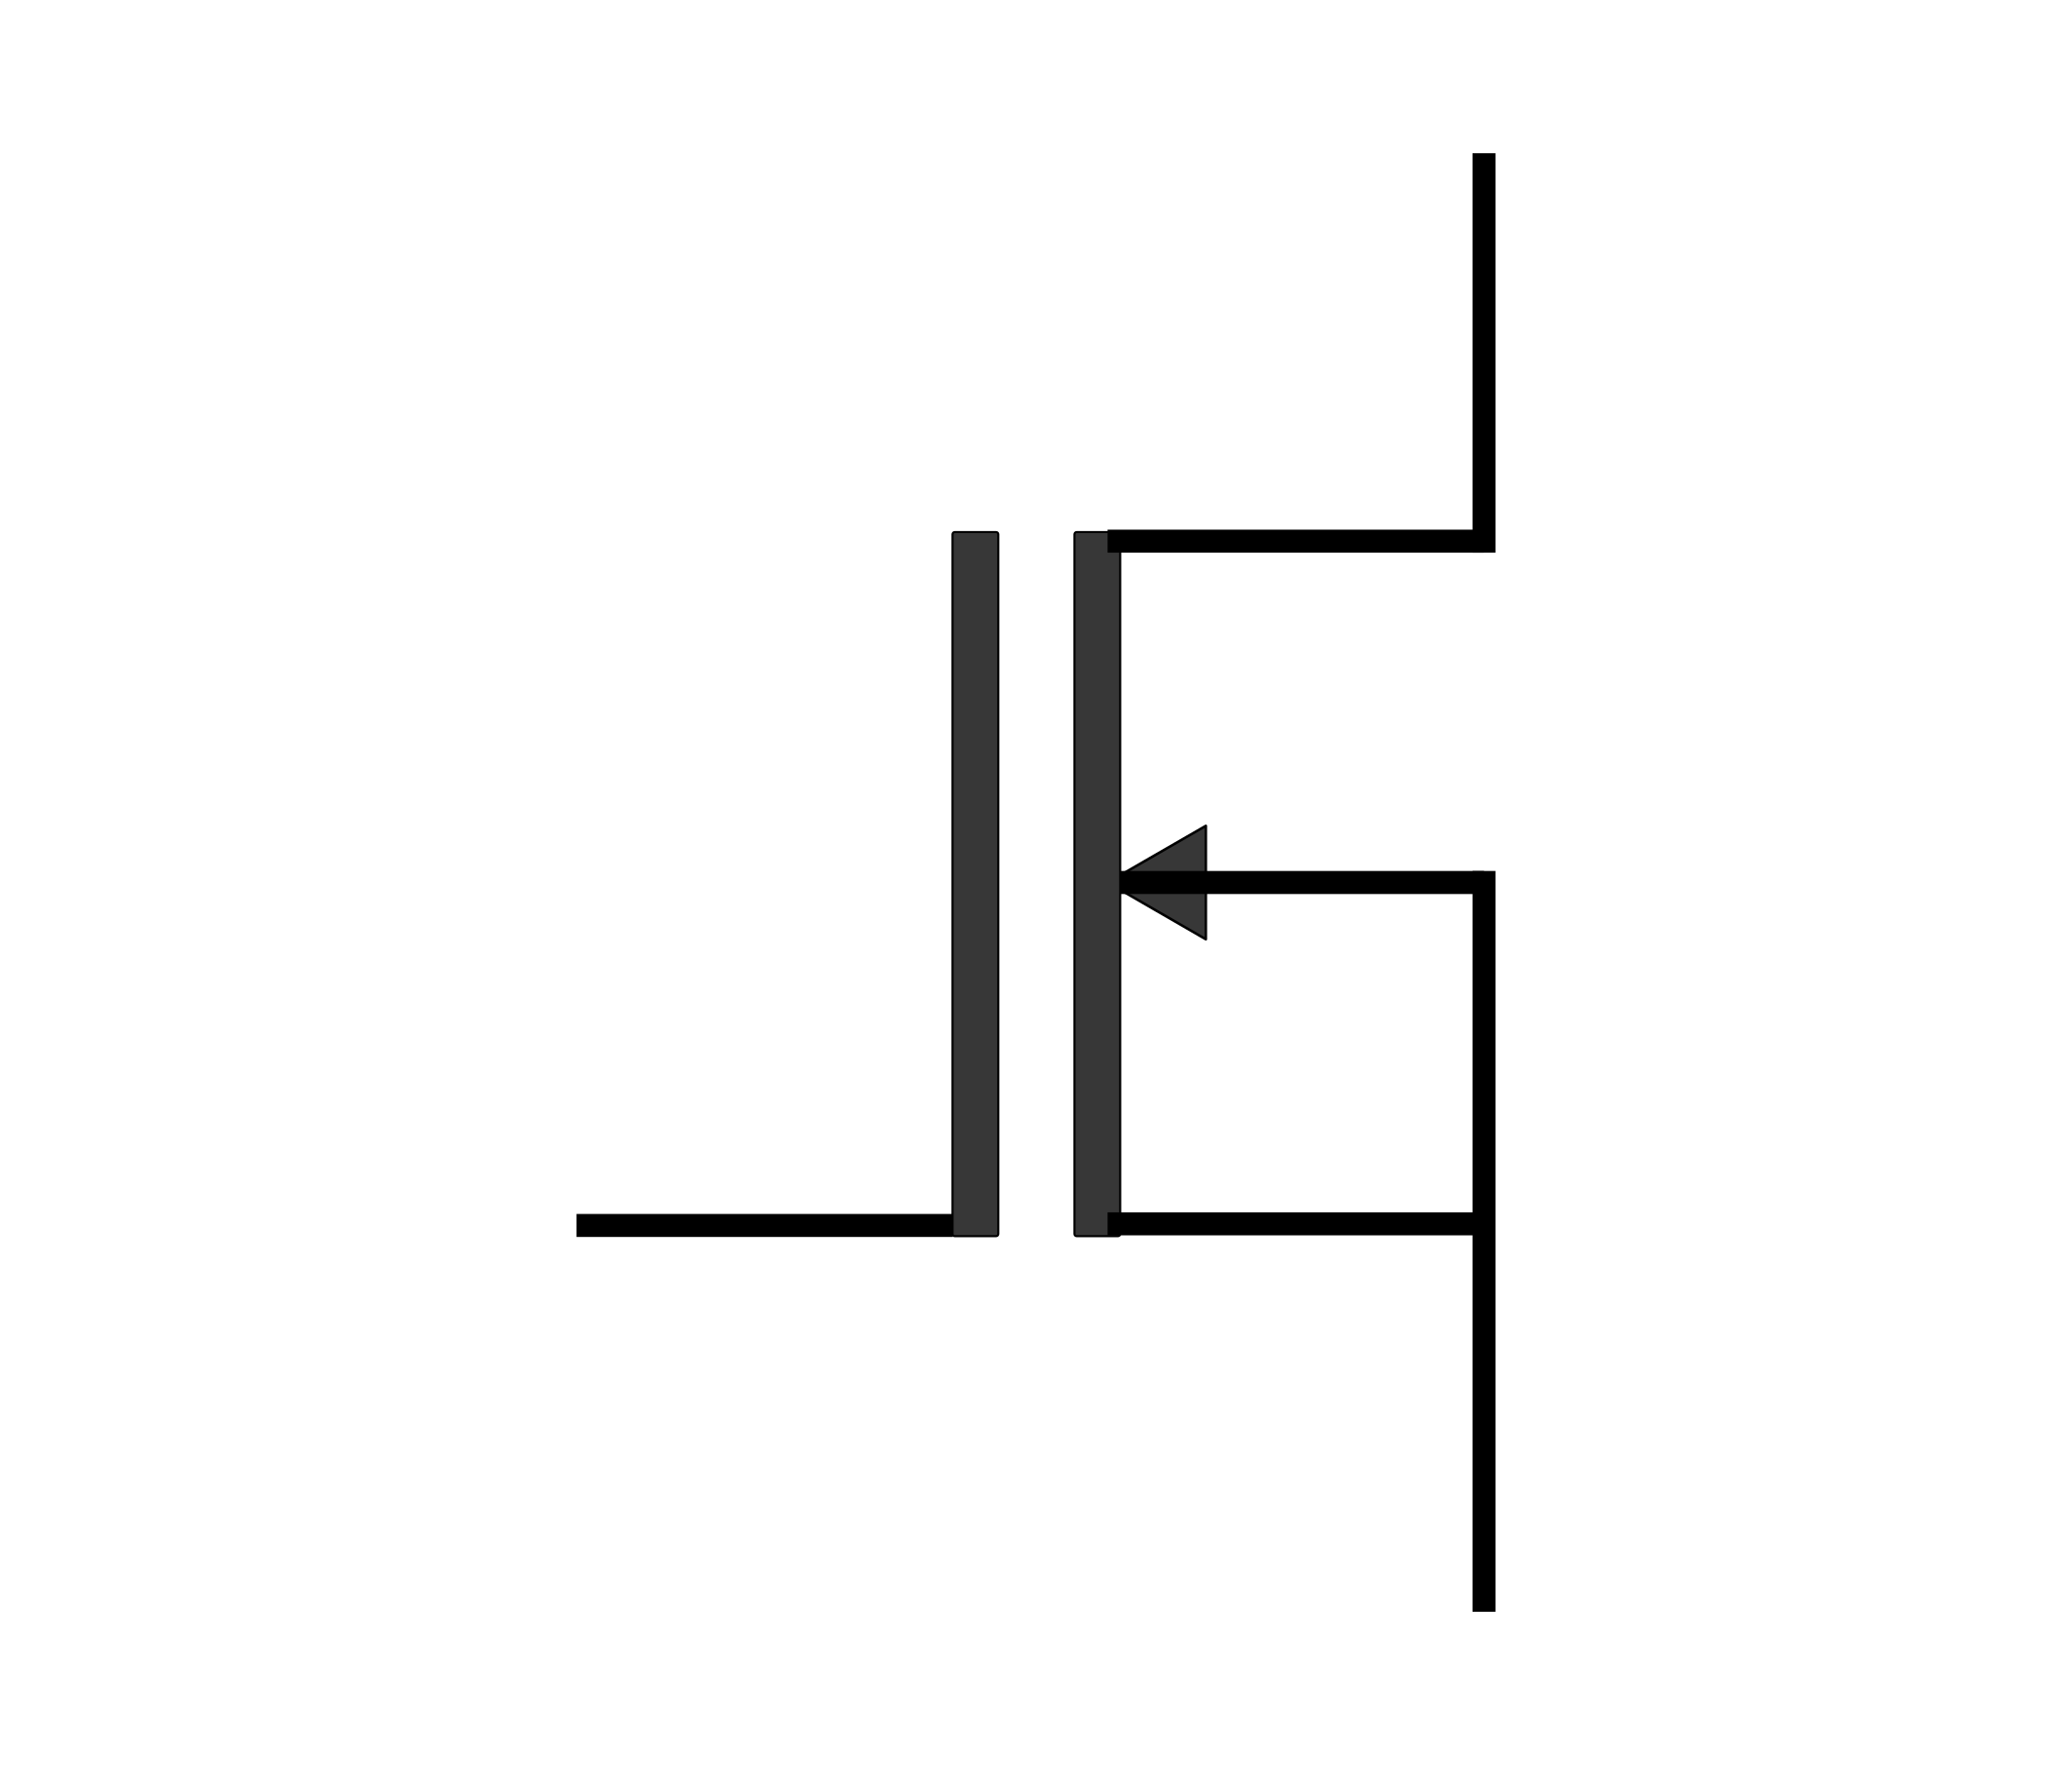
\includegraphics[width=0.4\textwidth]{MOSFET}
\caption{Metal-Oxide-Semiconductor Field Effect Transistor (MOSFET) representation}
\end{figure}

There are other switches, mainly for high power electronics, which don't require as much depth.

Relays are an alternate form of switch, which uses an \gls{elcmgnt} to cause a switch to open or close. Most switches work with \gls{drtcrt}, where relays are useful for \gls{atngcrt} applications. They are another form of switch that provides electrical isolation between parts, as it is an \gls{elcmgnt} which pushes the switch closed.

\begin{figure}[H]
\centering
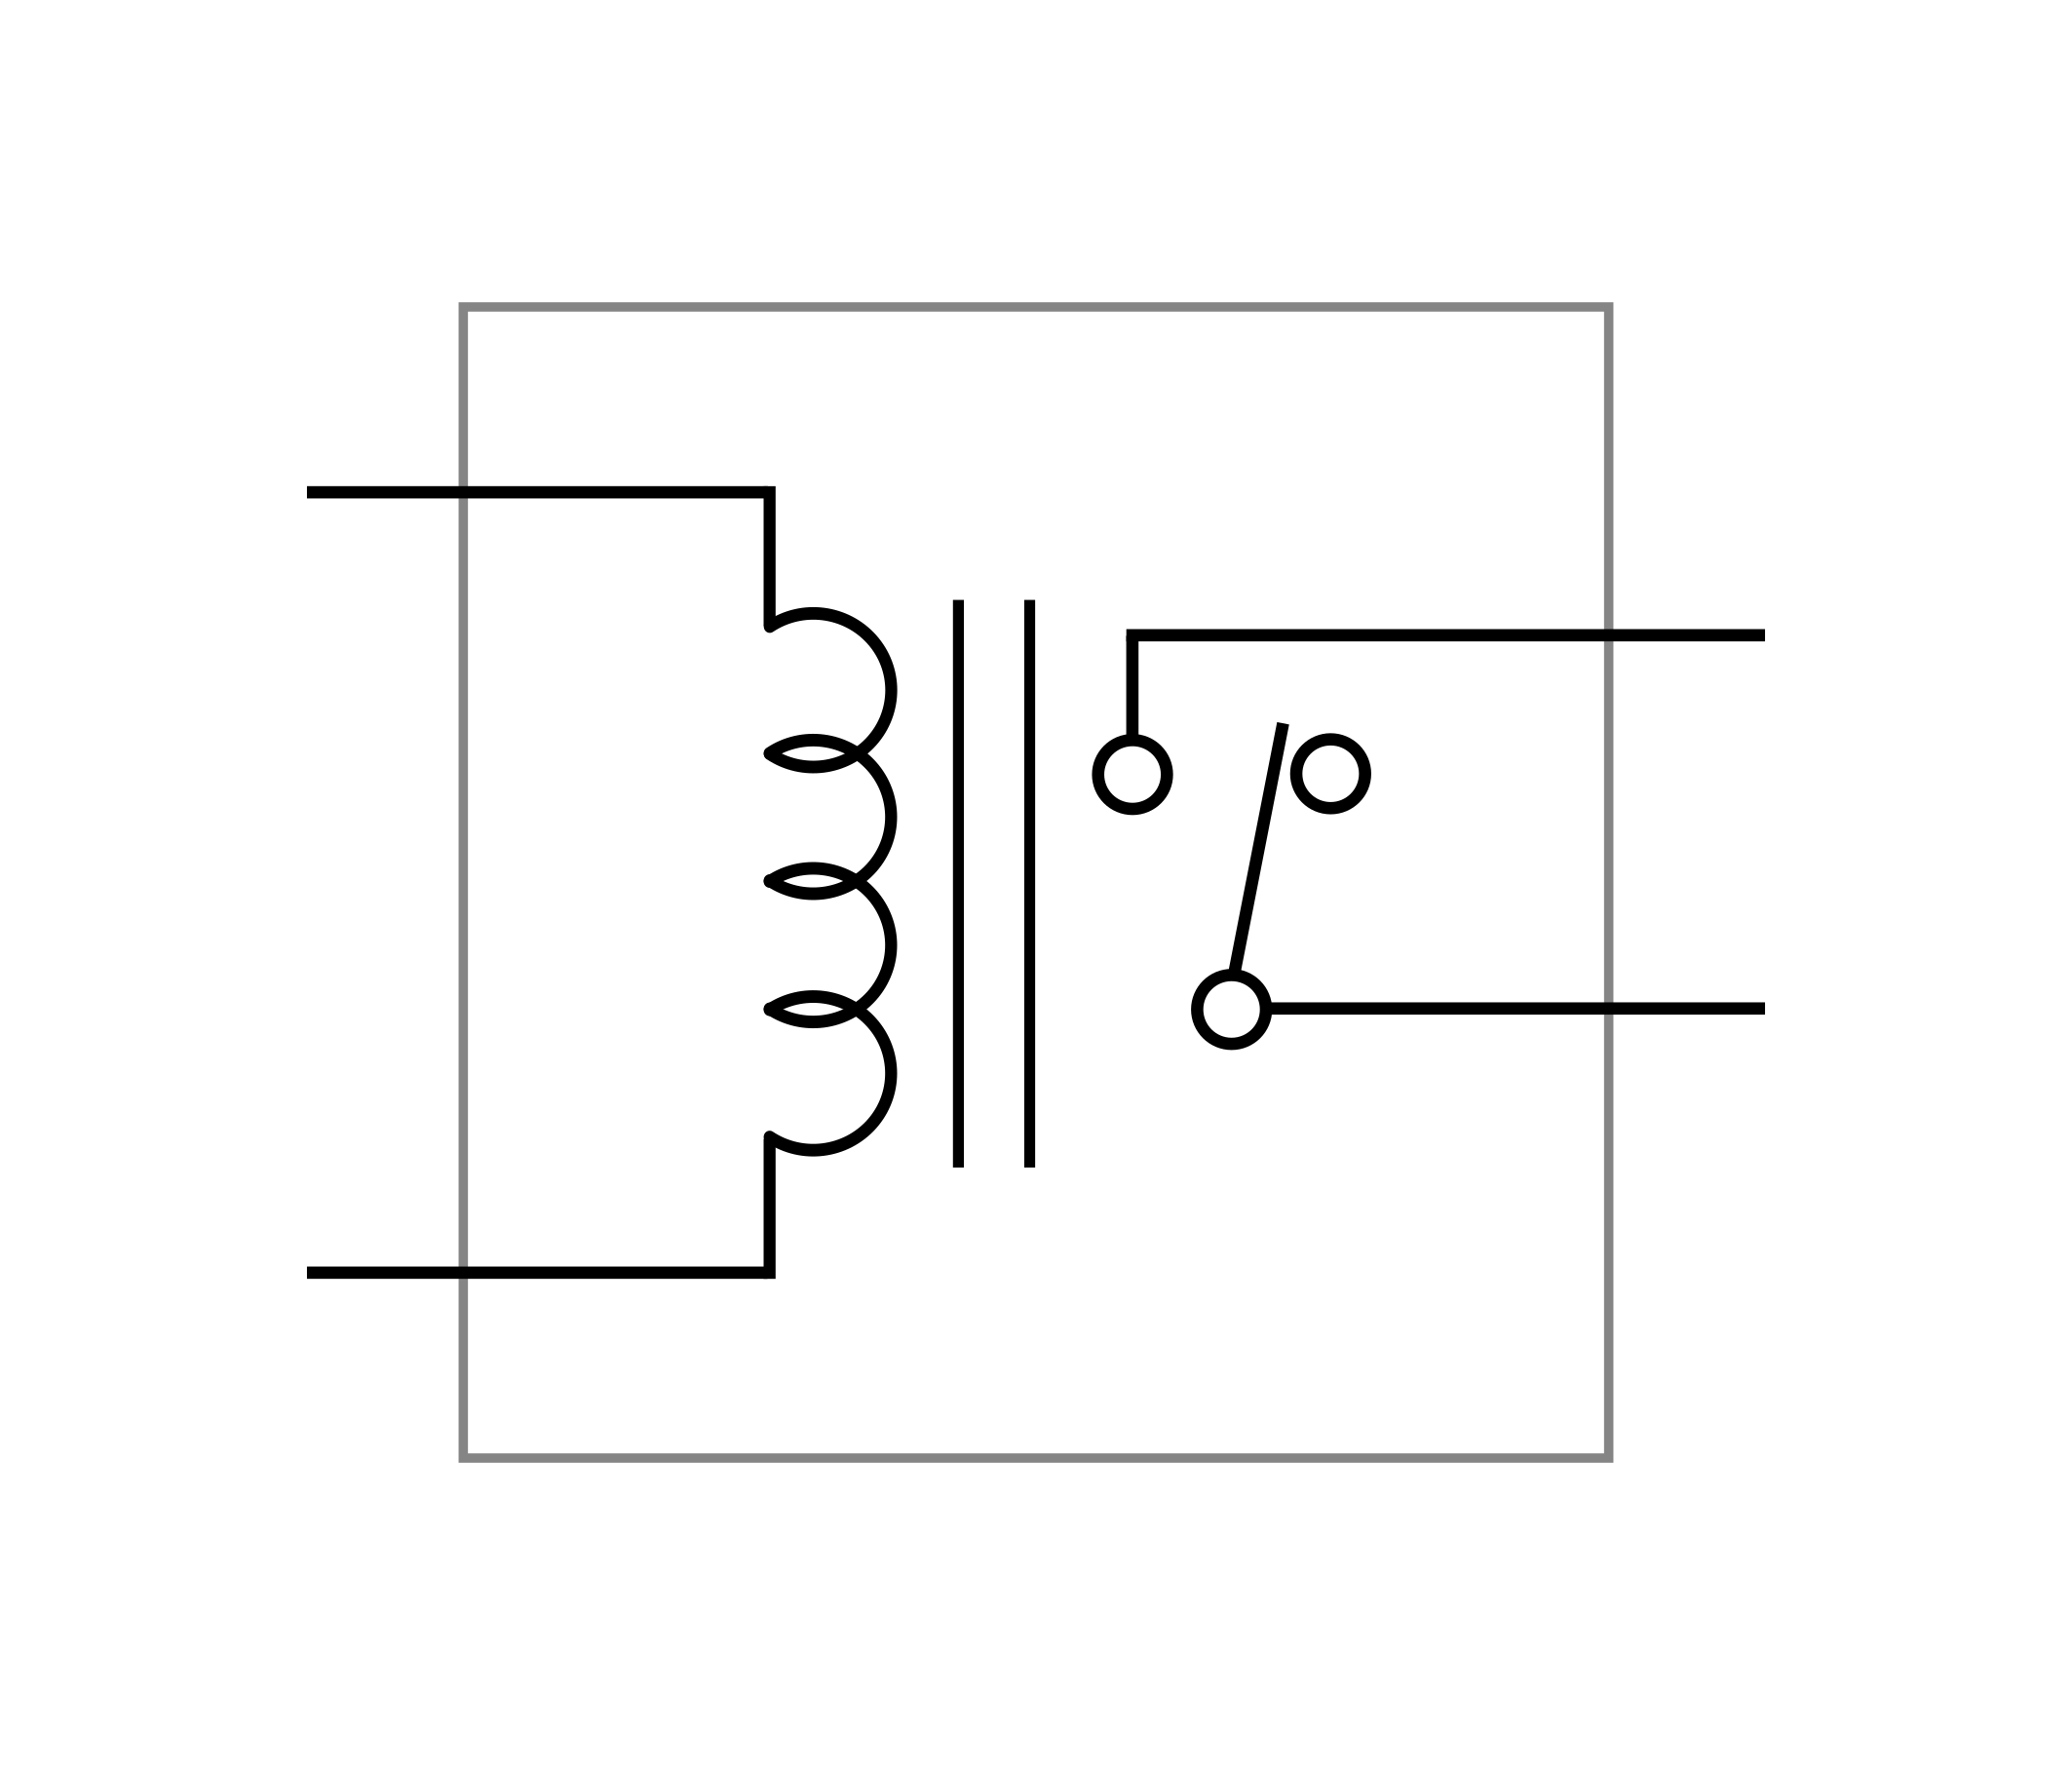
\includegraphics[width=0.4\textwidth]{relay}
\caption{Relay representation}
\end{figure}

Darlington \gls{trstr}s are also commonly known as a \gls{dlgtnpr}, made of a couple \gls{bjt} \gls{trstr}s, allowing higher levels of \gls{crnt} amplification/ high \gls{crnt} gain.

\begin{figure}[H]
\centering
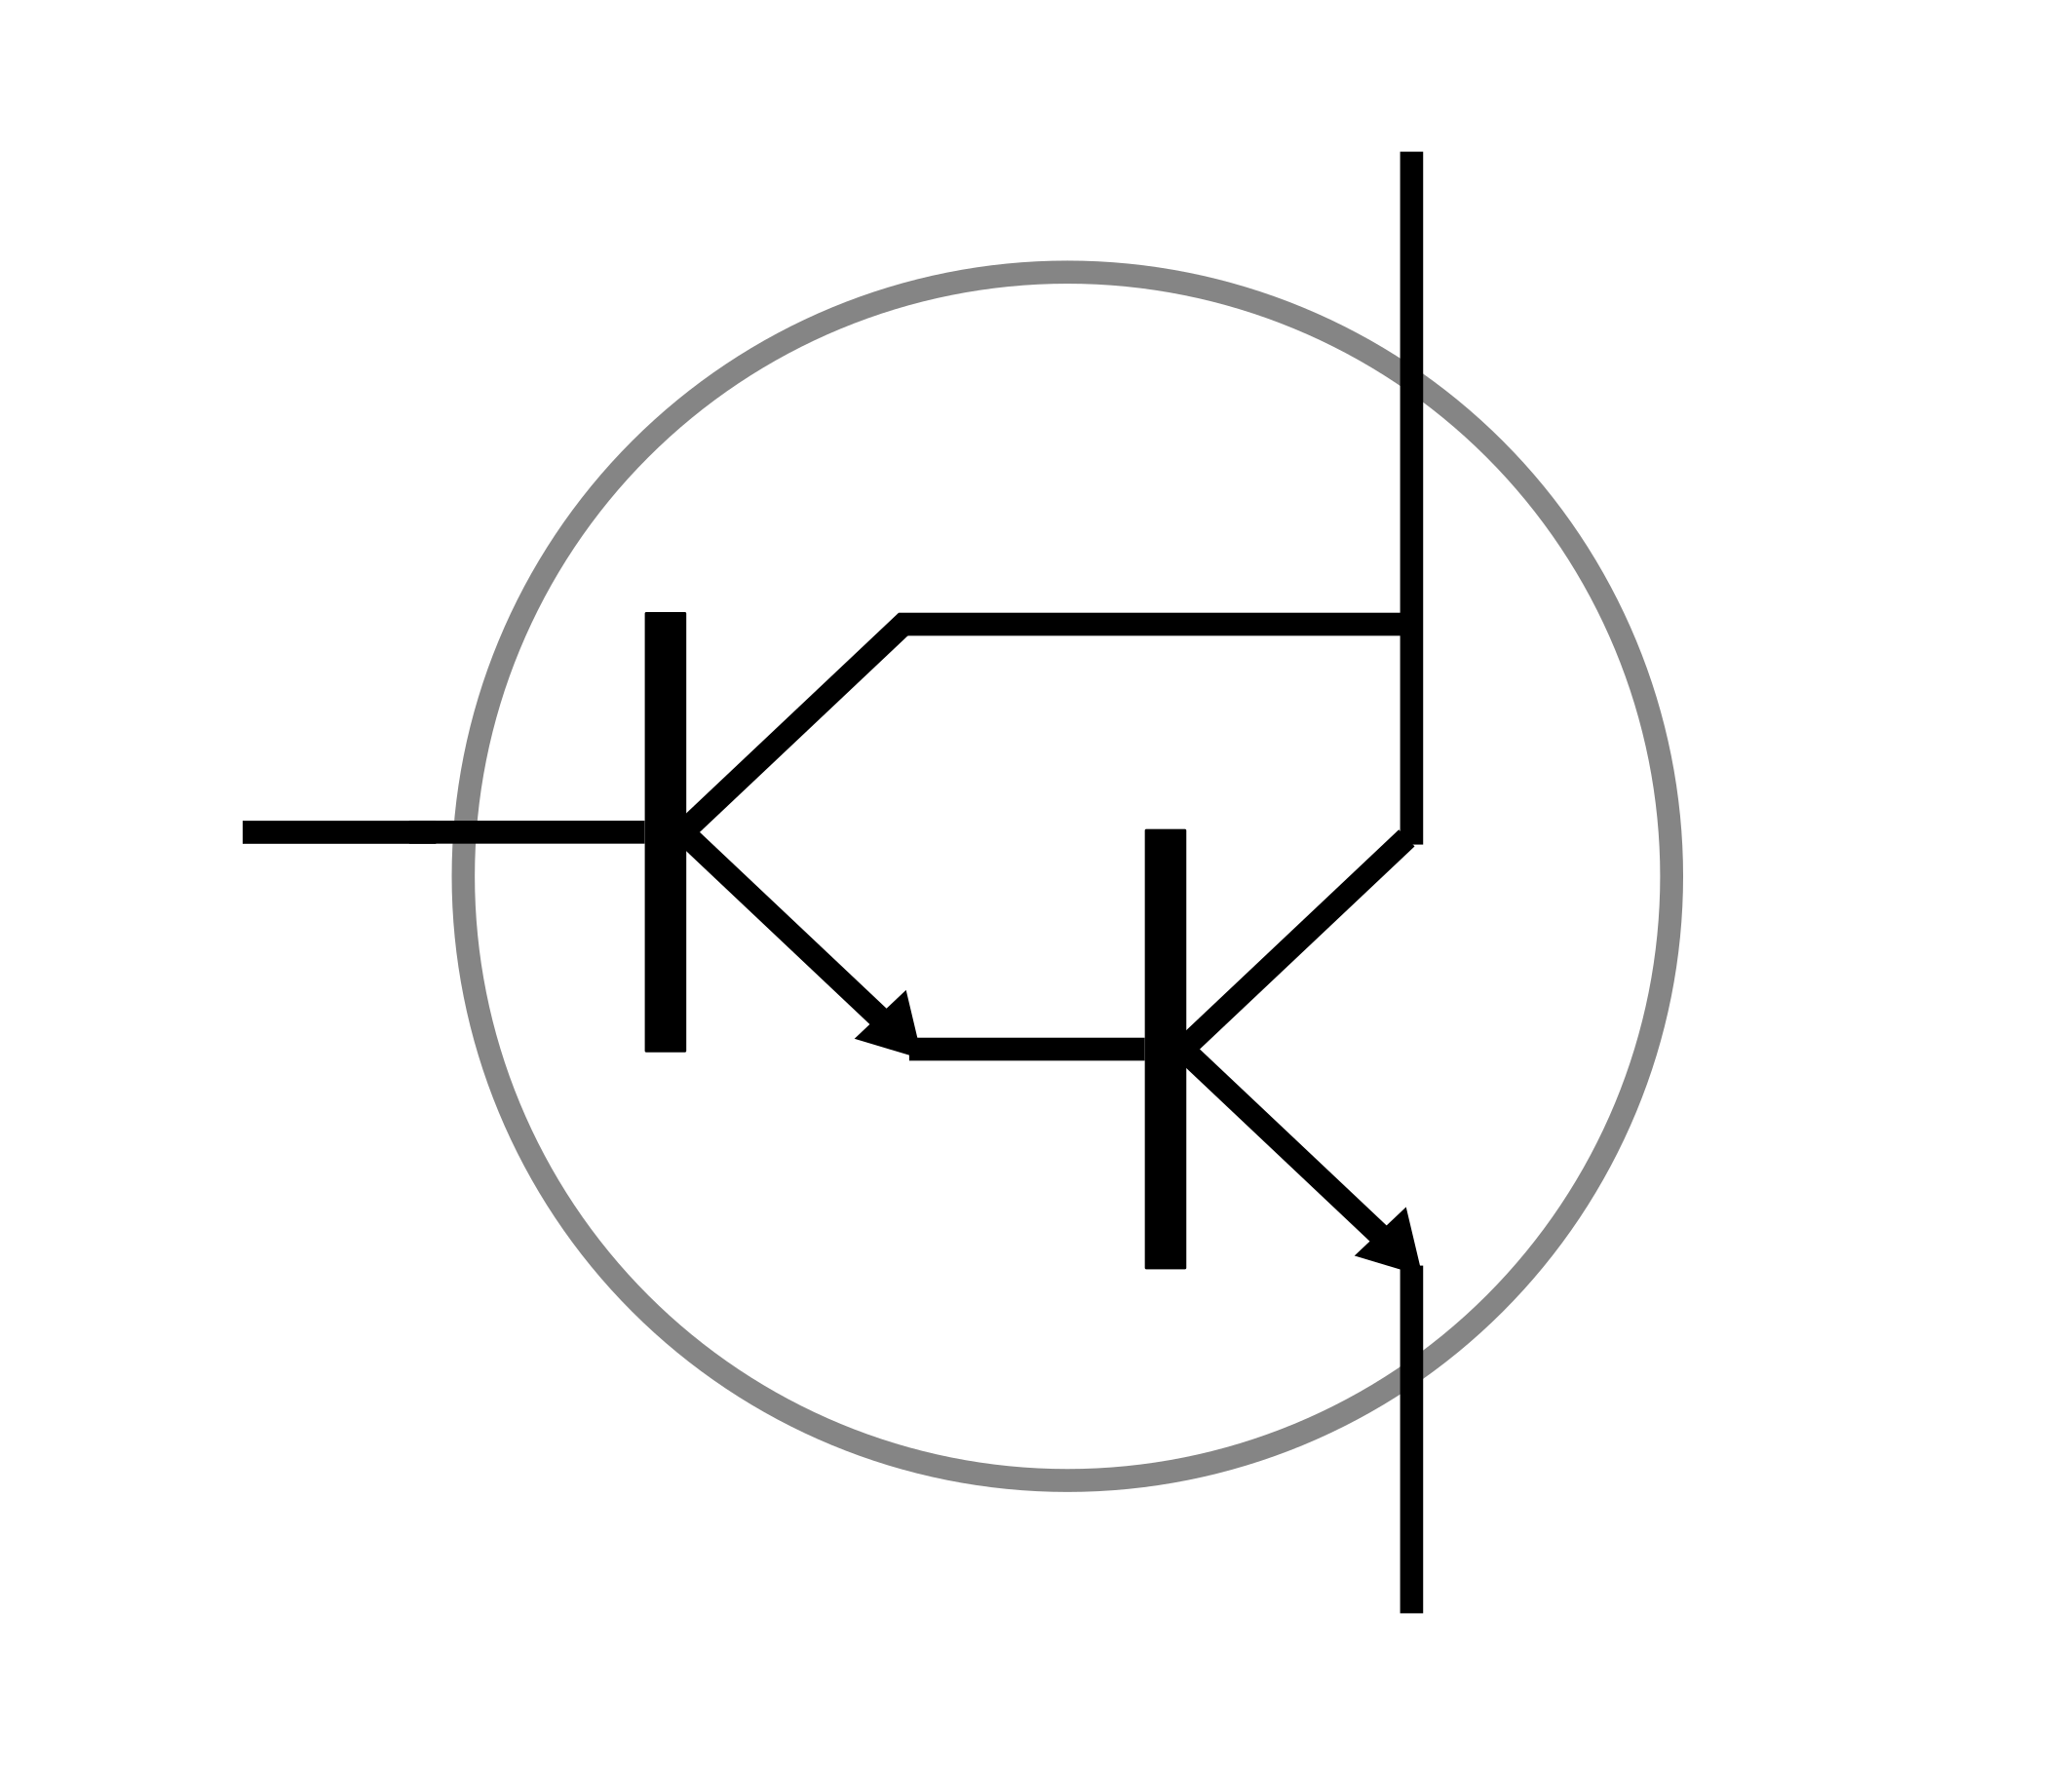
\includegraphics[width=0.4\textwidth]{darlingtontransistor}
\caption{Darlington Transistor representation}
\end{figure}

You can get arrays of \gls{trstr}s, such as Darlington Arrays, which is a chip with multiple Darlington \gls{trstr}s with common emitters. These are useful for high power or inductive loads being controlled by a \gls{micrctrlr}.

\begin{figure}[H]
\centering
\includegraphics[width=0.4\textwidth]{transistorpackages}
\caption{Common Transistor Packages}
\end{figure}

\Quiz{Quiz}

1. What type of \gls{dgtl} switch could you use for turning an \gls{atngcrt} \gls{mtr} on and off?

2. If you needed a simple \gls{trstr} circuit to turn a high power \gls{led} on and off from a \gls{micrctrlr}, what type of \gls{trstr} would you use and why?

3. What is the purpose of a \gls{trstr} \gls{gte}? Feel free to use an analogy to help you explain?

\vspace*{1\baselineskip}

\subsection{Sensors}

\Theory{What are \gls{snsr}s?}

\gls{snsr}s are likely to be a key component or \gls{modl} you use in your research, so understanding how they work and your options is important. Key aspects of \gls{snsr} theory are discussed here, with more in the further reading section.

This is split into several sections, covering some of the major \gls{snsr}s, with more detail on \gls{snsr}s likely to be used within chemistry related projects.

\gls{snsr}s typically use \gls{rstnc}, \gls{cptnc} or \gls{idtnc} to take a vast range of measurements, often using a MicroElectroMechanical system (\gls{mems}) to allow for this.

Temperature sensing can be done with a range of different methods, and is likely to be important. The most common \gls{snsr}s are \gls{anlge} ones, where the components \gls{rstnc} changes along with a temperature change, although there are \gls{dgtl} \gls{snsr}s for this too. There are 4 major categories of temperature \gls{snsr}, which we will quickly touch upon each. There are \gls{thrmcpl}s, \gls{rtd}s, \gls{thrmstr}s and specific \gls{dgtl} ICs.

\gls{thrmstr}s are common, and are divided into NTC and PTC, with NTC more common. NTCs have a decreasing \gls{rstnc} compared to temperature, and will have a \gls{rstnc} rating for 25\degree C typically along with a value for how much their \gls{rstnc} changes per degree. Therefore, utilising a circuit to measure this \gls{rstnc} allows for a relatively accurate temperature to be read. In comparison, PTCs have a positive temperature coefficient.

\gls{rtd}s are similar in their operation to \gls{thrmstr}s, but are meant for a wide range of temperatures, upwards of around 600C. Many consist of a length of thin wire wrapped around a ceramic or glass \gls{core}.

A \gls{thrmcpl} consists of two differing conductors which generate a temperature dependant \gls{vltg}. They have the highest temperature range of temperature \gls{snsr}s, upwards of around 1800C.

\gls{dgtl} temperature ICs will measure a temperature and report the data through a specific \gls{prtcl}, which is discussed further (here).


Humidity \gls{snsr}s may be used along with temperature \gls{snsr}s, in a single package. The output can be \gls{dgtl} or \gls{anlge}. A couple of common \gls{dgtl} examples include the DHT11, DHT22 and AM2320.


There are many \gls{snsr}s for detecting compounds in the air, important for atmospheric research. Usually these are \gls{dpd} so that a higher concentration of a certain gas, such as carbon dioxide, induces a \gls{vltg}. Because of the calibration involved and comparison with data, they are often complex ICs, which communicate via a \gls{prtcl} such as \gls{i2c} or \gls{spi} to a \gls{micrctrlr}, discussed in the \gls{prtcl}s section. Although certain \gls{snsr}s may leave the conversion to the user. More \gls{modl}s are appearing in the market, helpful for taking more reliable measurements.


Photo\gls{rstr}s use a similar method for light, where a \gls{rstnc} is associated with pitch black, and separately for light. Therefore, an estimated light intensity will be attained, with a given \gls{vltg}. There are also photo\gls{diod}s and photo\gls{rstr}s, each with their own benefits, like higher response rate, or lower costs.


There is a range of movement based \gls{snsr}s, which will quickly be touched upon. You are unlikely to need to use these much.

One of the main cheap and widely used range/ movement \gls{snsr}s is an \gls{ultrsnc} \gls{snsr}, which has an \gls{ultrsnc} transmitter and receiver. This uses knowledge of the speed of sound, to measure the time it takes for sound to hit a surface and reflect, to then calculate a distance value.

There are also \gls{lidr} \gls{snsr}s, which are similar but known to have higher precision, which use a singular beam of light, and calculate its time of travel. These are also known as Time of Flight (ToF) \gls{snsr}s.

The motion based \gls{snsr}s discussed above are ones that are contactless, but there are also contact based \gls{snsr}s, which a \gls{ptmtr} could be an example of, using its \gls{rstnc} based on a linear or rotational movement as a measurement of movement.

\begin{figure}[H]
\centering
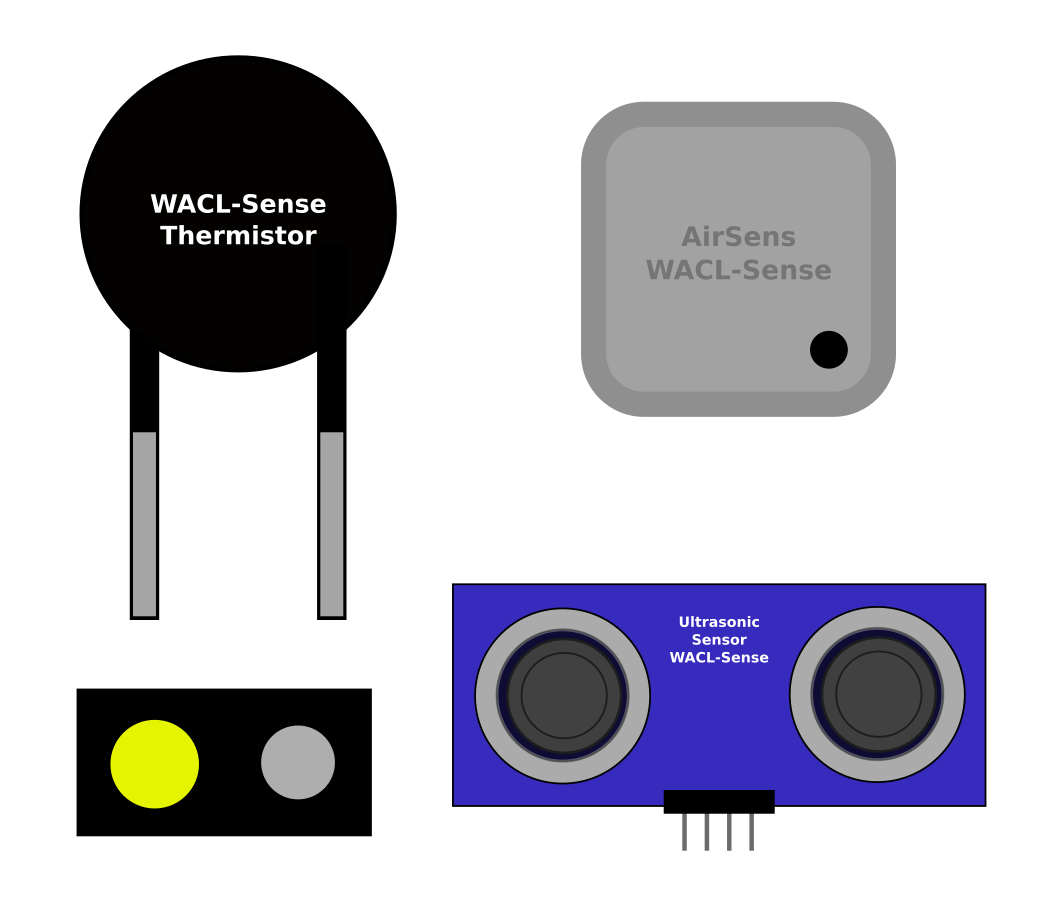
\includegraphics[width=0.4\textwidth]{SensorPackages}
\caption{Example Sensor Packages}
\end{figure}

\Examples{Examples}

At this point you have seen a good proportion of components, to have more complex examples. Coming back to the heater suggestion mentioned earlier in the document, but this time there could be a control loop factored in. We will assume a the processing is all sorted by a \gls{micrctrlr}. We can use the same resistor/ heating element of 2000W, but will use a \gls{trstr} to turn it on and off. For simplicity, and since a small voltage drop should not have a massive effect, a \gls{bjt} could be selected here. The \gls{bjt} could be triggered to turn off when the value from an \gls{anlge} \gls{thrmstr} correlates to a higher temperature than what has been selected as the required temperature. It could be a potentiometer which is used as a temperature knob.

\Quiz{Quiz}

1. What is the difference between a NTC and a PTC \gls{thrmstr}?

2. What type of temperature \gls{snsr} would you choose for a furnace, with temperatures as high as 900\degree C.

3. If you needed to precisely measure a distance, what would be a good \gls{snsr} choice?

4. Name a couple of \gls{prtcl}s that \gls{snsr}s may communicate with?

\vspace*{1\baselineskip}

\subsection{Optoisolators}

\gls{optisltr}s, otherwise known as optocouplers, are components that use light to transfer electrical signals between two isolated circuits. This is important if the two circuits need differing \gls{vltg}s, or need isolating.

They use an \gls{led} and a photo\gls{snsr}/ photo\gls{trstr}, so it is light that transmits the signals, which keeps them electrically isolated. They are useful for measuring \gls{atngcrt} using \gls{drtcrt} electronics, so have uses within \gls{atngcrt}-\gls{drtcrt} power conversion/ supplies.

It may be worth reading the sections on photo-\gls{snsr}s/ photo-\gls{trstr}s within \gls{snsr}s, as well as \gls{trstr}s and \gls{diod}s, to fully understand this.

\begin{figure}[H]
\centering
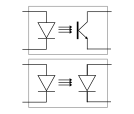
\includegraphics[width=0.4\textwidth]{optoisolator1}
\caption{Optoisolator representations, phototransistor varient on top, photodiode varient below}
\end{figure}

\Quiz{Quiz}

1. Name an application where an \gls{optisltr} would be helpful?

2. What components are within an \gls{optisltr}?

3. Are \gls{optisltr}s suitable for transferring a lot of power?

\vspace*{1\baselineskip}

\subsection{Power Sources}

It is important to consider what power source you should use for a given project.

Batteries come in many different types, some being rechargeable chemistries and others not. Many batteries use lithium, a very common material for rechargeable batteries, although it requires careful consideration and the use of a charge IC, to ensure that both its environmental and operating conditions are suitable. If not used wisely, it can be a dangerous chemistry with a range of risks stemming from mishandeling, shorts, over and undercharging and more.

\begin{figure}[H]
\centering
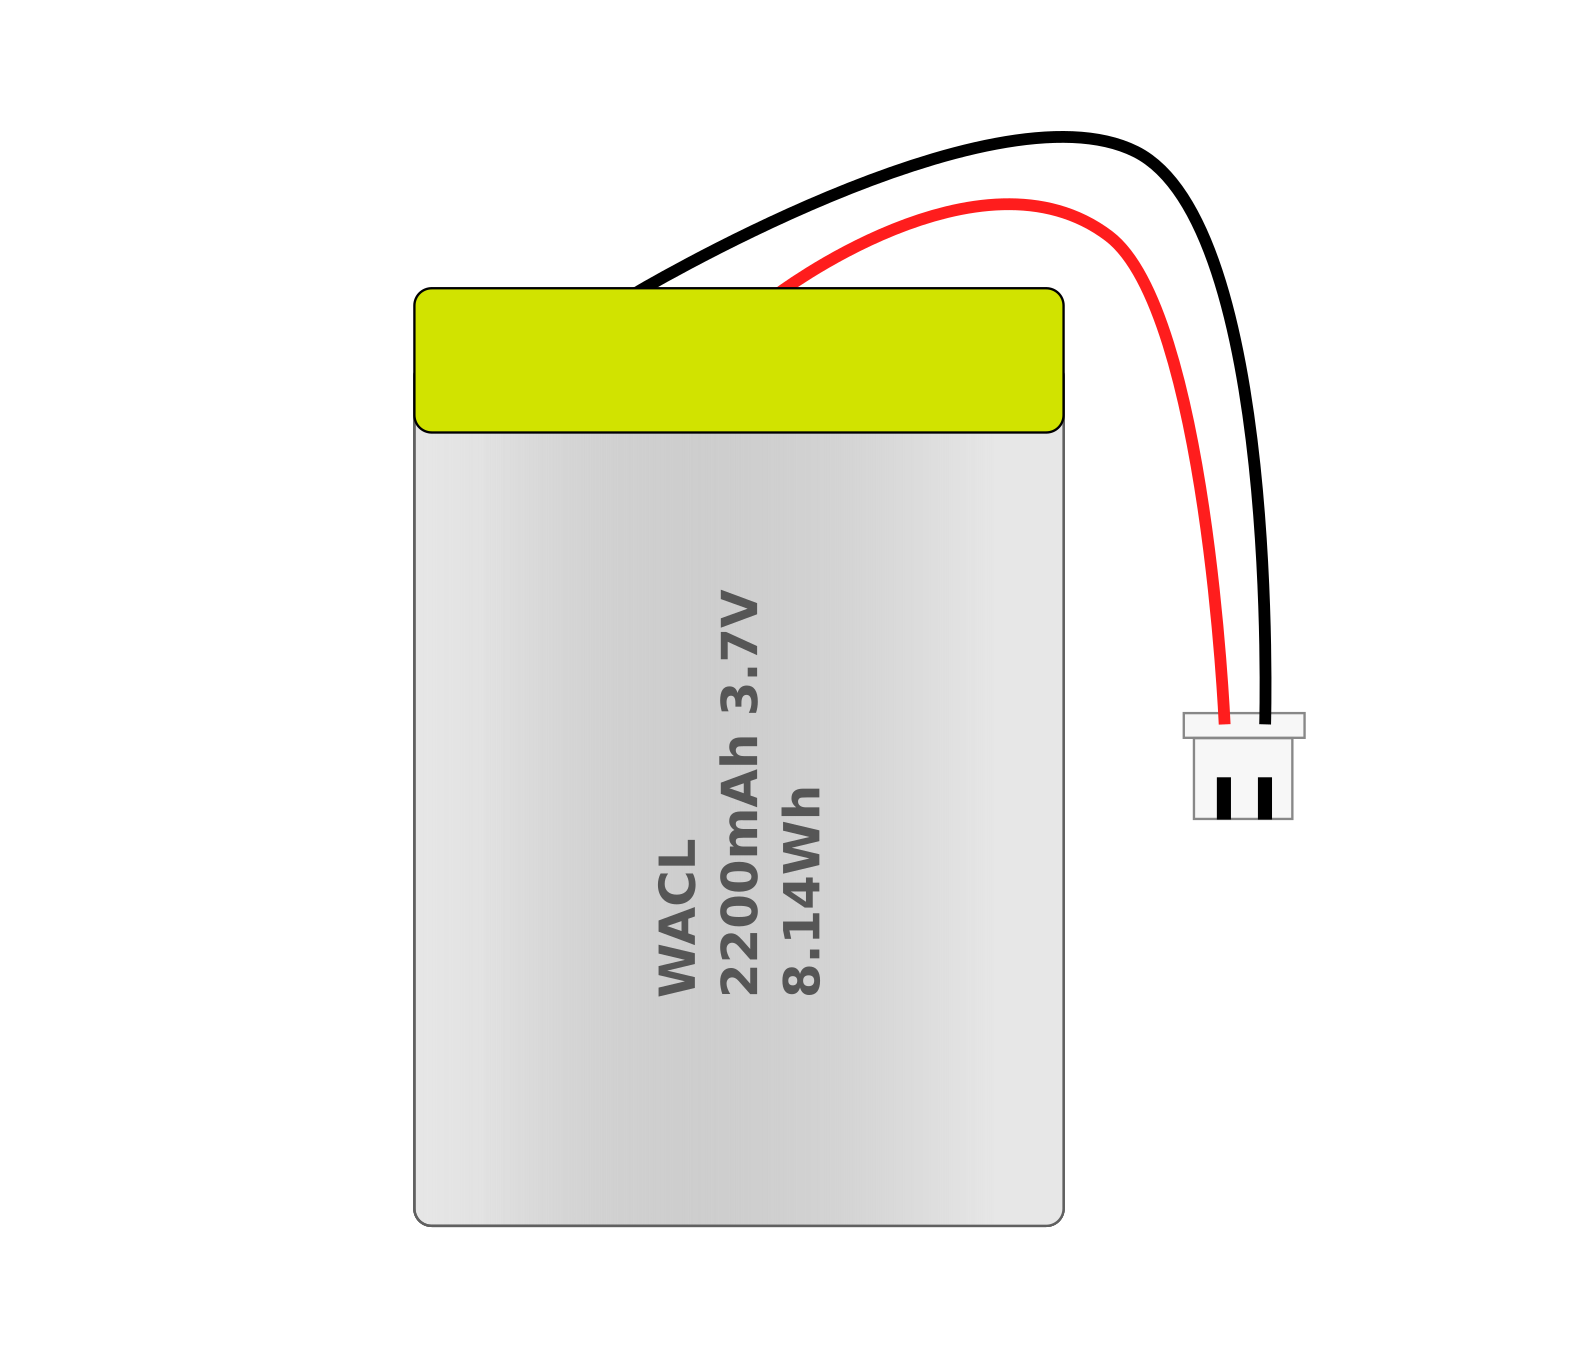
\includegraphics[width=0.4\textwidth]{lipobattery}
\caption{Example Lithium Polymer (LiPo) battery}
\end{figure}

There are a few more forgiving rechargeable battery chemistries, one of the main ones being NiMH, which has characteristics in a similar magnitude to lithium cells, although generally worse in both energy and power density. Energy density is the amount of energy it can store either per litre or kg, so will affect how long a product will last, where power density is the magnitude of power it can continuously supply, again either per litre or kg. Energy density is given in Wh, which is the number of \gls{wt}s of energy it could supply for an hour.

NiCD and Lead Acid are two other battery chemistries which still get some use, but are decreasing in relevance due to them having worse characteristics in a range of aspects, and poor carbon footprint. Lead acid is still used for certain applications due to how easy it is to charge and discharge, and its low cost per Wh.

Common non-rechargeable battery chemistries include alkaline and zinc carbon. Alkaline tends to provide more energy, and tends to use lower pollutants, so should be the better choice than zinc carbon unless a very low budget is a key constraint. So other than costs, I would say use of rechargeable battery chemistries would be best in most cases.

Along with battery sources, considering wired methods are also useful. \gls{usb} is one of the more common methods, with most \gls{usb} methods transmitting 5V. \gls{usb} C for example allows for devices to "negotiate" their \gls{vltg} draw, between 5-20V, with a 5V default. Micro \gls{usb} B, which used to be a standard for portable devices in some cases can handle a max of 3A, where \gls{usb} C can handle up to 5A, making it suitable to power many projects. The connector has a higher durability, and can be inserted either way. Other data transfer can be done through it as well, making it versatile.

\gls{drtcrt} \gls{jck}s are useful for power only, and can vary in dimensions and power output. It is fairly common to get \gls{drtcrt} \gls{jck} based power supplies with 6V, 12V and 20V \gls{vltg} outputs, with a range of \gls{crnt} outputs.

Adjustable \gls{drtcrt} power supplies are helpful for testing stages, or if specific \gls{vltg}s are needed, and will power a device with \gls{vltg}s between around 0-30V and sometimes 0-60V or more. 5A and 10A are both fairly common for max \gls{crnt} output capabilities.

Supplementory power methods include the use of a \gls{mtr} as a \gls{gnrtr} or a solar panel, spoken about later. Alow energy density battery alternative with quick charging capability is a \gls{sprcpctr}, suitable for very low power applications, potentially topped up with a solar panel.

\Quiz{Quiz}

1. A temperature sensor for remote use needs to be made, where it takes a measurement once an hour, with someone manually retrieving data once a week. Name a power source which might be suitable?

2. Why are lead-acid batteries still used, and why are they not very goof for a lot of cases now?

3. A device for lab use needs a specific voltage of 27.6V to run. What do you think a good choice would be to power it?

4. What is commonly known as quite a safe battery chemistry?

5. What is good about \gls{usb} C?

\vspace*{1\baselineskip}

\subsection{Ideal vs Non-ideal Components}

Until now, we have talked about components as if they are ideal. This means they have no losses other than expected. In reality, components have internal \gls{rstnc}, \gls{cptnc} and \gls{idtnc}. For low-speed circuit design, the internal \gls{rstnc} is what you mainly need to be aware of. This includes the source, with certain batteries/ sources having a high internal \gls{rstnc}, which means at higher \gls{crnt} draws, there can be a fairly significant \gls{vltg} drop before it even gets to the rest of the circuit. Any of these factors can have a significant effect upon a more high-speed circuit, with \gls{cptnc} and \gls{idtnc} altering over different frequencies. In high speed circuit boards, there are a range of techniques used to limit the potential for unwanted \gls{cptnc} and \gls{idtnc} to affect a circuit. Issues such as this could be what causes circuit problems, especially for breadboard designs. These are often known as \gls{prstcs}, which are undesirable characteristics affecting components or the circuit.

Because of factors such as the above, component functions don't always happen instantaneously, such as there being a turn on/ off or switch on/ off time for a given component.

A battery/ power source would usually have an ESR value, which stands for equivalent \gls{srs} \gls{rstnc}. This is important to consider what losses, heat build up and \gls{vltg} drop could be seen at particular loads.

It is also beneficial to know the term \gls{impdnc}, which is the effective resistance of an AC circuit, being a combination of both resistance and \gls{ractnc}. As mentioned above, circuits will have a level of inductance and capacitance, which causes \gls{ractnc} in an AC circuit.

\Quiz{Quiz}

1. True or false, real world components can be thought of as non-ideal?

2. What characteristics do non-ideal components have, which may cause issues for certain circuits?

3. True or false, non-ideal components tend to be more of a problem for low-speed circuits.

\pagebreak

\section{Power conversion}

Power conversion could be its own course, so this lightly touches upon conversion for a base understanding and why it is important. Within the further reading section, there is information on \gls{rectfctn}, combining theory above, so is worth checking for more of a challenge, or if \gls{atngcrt}-\gls{drtcrt} conversion knowledge is necessary.

The main types of power conversion are active and linear. Active utilises both \gls{cptr}s and \gls{indctr}s, as well as switches for efficient conversion of \gls{vltg}, either to a higher or lower level, with efficiencies into the 90\% possible. Whereas linear power conversion is cheaper, requires a lower number of components and is specifically for decreasing the \gls{vltg} at the output. It acts as a variable \gls{rstr}, to dissipate the unwanted \gls{vltg} as heat, so depending on the circuit's needs, can be particularly inefficient. Therefore, if efficiency is less important than costs, or the \gls{vltg} decrease is only very minimal, linear \gls{vltg} converters can be an okay option. Given how easy it is to find power conversion \gls{modl}s (either known as step-up or step-down, whether \gls{vltg} is increased or decreased), these are usually better than custom designs, as usually only a \gls{ptmtr} needs altering to get necessary output \gls{vltg}, with minimal losses.

For a quick active power converter insight, a switch is turned on at set ratios to charge an \gls{indctr}, which then discharges to charge a \gls{cptr} for a smoothed \gls{vltg} at the intended level. The ratio between the switch on and off times will affect the output \gls{vltg}.

The above mainly discussed \gls{drtcrt} to \gls{drtcrt} power conversion. To do \gls{atngcrt} to \gls{atngcrt}, a \gls{trnfmr} is commonly used. \gls{atngcrt} to \gls{drtcrt} may use a similar method to the above but using a \gls{trnfmr} rather than an \gls{indctr}, and the use of a \gls{rectfir} to convert the \gls{atngcrt} to \gls{drtcrt}.

\Quiz{Quiz}

1. Name three other types of conversion if the example is \gls{drtcrt} to \gls{drtcrt}.

2. True or false, active power conversion is always more efficient than linear power conversion?

3. True or false, it is typically recommended to use a \gls{modl} for active power conversion due to their design complexity?

4. What would the efficiency be of a linear power converter, converting an input of 5V down to 3.3V?

5. For a variable load circuit, which runs off 3V and has a 3.3V supply, would a linear regulator be a good option, and why?

\pagebreak

\section{Communication Protocols}

\vspace*{1\baselineskip}

\subsection{Wired Communication Protocols}

Communication \gls{prtcl}s are important to interface with different devices and equipment, so a base understanding of some of the major ones would be important.

Communication \gls{prtcl}s are a set of rules which devices follow to transfer information, allowing coherent data transfer at set speeds, depending on the use case.

It will first be useful to distinguish between \gls{srl} and \gls{prl}, since these are widely referenced regarding communication \gls{prtcl}s.

\gls{srl} means that there is a single data line/ wire used for communication in a given direction, where \gls{prl} means that there are several data lines or wires with data travelling through. Therefore, \gls{srl} is often an easier method to use or implement.

They can first be split into two main kinds, with inter system \gls{prtcl}s being those used to have communication between devices, where intra system communication \gls{prtcl}s are meant for between component communication.

Therefore, you may use a combination of the two, depending on the project.

It is useful to know the term Port. Ports are points where communication can be done from, to a specific device.

\gls{usb} and \gls{urt} are the main examples of inter system \gls{prtcl}s, where \gls{spi}, \gls{i2c} and \gls{can} are some of the main intra system \gls{prtcl}s. Although some of the main \gls{prtcl}s, it is not a definitive list, with niche or proprietary \gls{prtcl}s being around. These may have specific benefits, or are proprietary to limit use of other companies' chips for a given application.

Master and Slave are still common terms within communication \gls{prtcl}s, that you need to be aware of, although there is a shift to alternate terms such as controller and responder, although not yet standardised. Other alternatives could include primary and secondary, leader and follower and source and sink, although the latter of which already is widely used within electronics. Because of the negative connotations of master and slave, this course uses the suggested terms of controller and responder. I2C is an example interface where the Master and Slave terms have officially been replaced with Controller and Target, although it may take some time for this to be fully recognized.

\gls{usb} is very widely used and is how many devices are connected to computers. It is high speed, and quite simple to implement, although requires the use of specific \gls{drvr}s and a powerful controller. \gls{usb} 1 and 2 have 4 pins, one for power, one for ground and two for data, with data being sent \gls{srl}ly in each direction.

\gls{urt} is physical circuitry for conversion between \gls{srl} and \gls{prl} data, where two \gls{urt}s may communicate with each other, communicating in \gls{srl}, meaning that only two wires/ data lines are necessary for communication between two devices.

\begin{figure}[H]
\centering
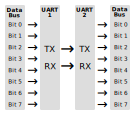
\includegraphics[width=0.4\textwidth]{UART}
\caption{UART Protocol diagram}
\end{figure}

\gls{r232} is another \gls{prtcl} (Recommended standard 232), which is often used within telecommunications. In general, it is often used for connecting devices such as data acquisition or modems, the prior of which are likely to be particularly important. On creation, \gls{r232} allowed for "handshaking", a method for checking that data is transmitting correctly, although many devices no longer require the use of this. \gls{r232} can directly connect to the \gls{srl}\gls{prt}of a computer.

\gls{mdbs} is a \gls{prtcl} which was created for communication for programmable logic controllers, often for industrial use. One reason for its wide usage is that it has no royalties and is open.

\gls{spi} is a commonly used \gls{prtcl}, which has a single controller and multiple responders connected to it. \gls{spi} stands for \gls{srl} Peripheral Interface, with there being 4 main lines used, two pins for data transfer, a pin for selecting which responder the controller is communicating with and a line used as a clock. Therefore, for each responder that the controller wants to communicate with, a separate select pin is required. It is a relatively fast communication \gls{prtcl}, but doesn't scale the best due to needing a new \gls{gpio} pin for each new device.

\begin{figure}[H]
\centering
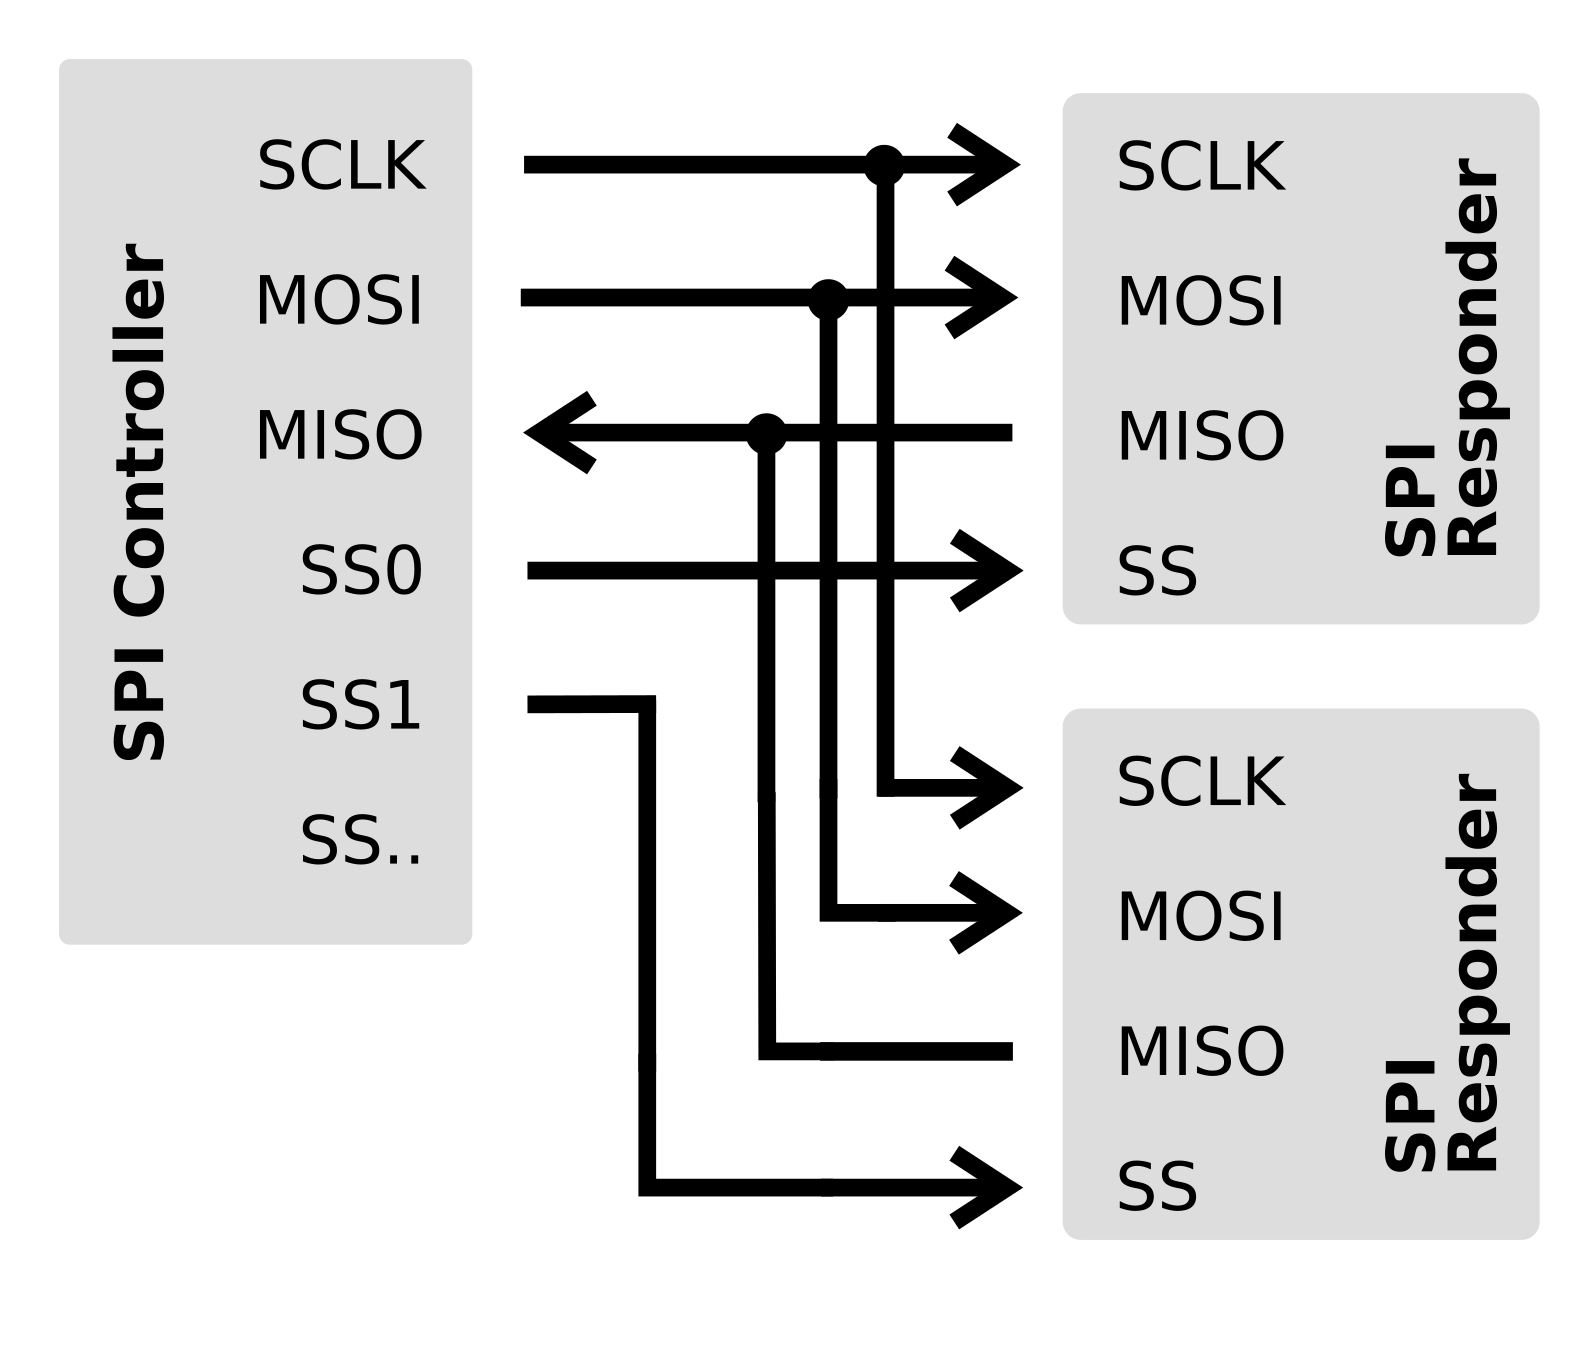
\includegraphics[width=0.4\textwidth]{SPI}
\caption{SPI Protocol diagram}
\end{figure}

\gls{i2c} is a similar \gls{prtcl}, which is also \gls{sycns}, like \gls{spi}, controlled with a clock from the controller. It only requires two wires for communication, the clock and the \gls{srl} data line. It can communicate with many devices/ responders with just two wires, but is limited in speed and has a combined transmitting and receiving data line.

\begin{figure}[H]
\centering
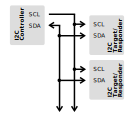
\includegraphics[width=0.4\textwidth]{I2C}
\caption{I2C Protocol diagram}
\end{figure}

\gls{can} stands for Controlled Area Network, and is a \gls{prtcl} meant for the transmission and receipt of data within a network of devices, especially for harsher environments. Due to this, it is mainly used in industrial and automotive environments, so may be used by certain research equipment. It is fast, secure and low cost, but is complex and automotive orientated.

\begin{figure}[H]
\centering
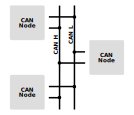
\includegraphics[width=0.4\textwidth]{CAN}
\caption{CAN Protocol diagram}
\end{figure}

Since not all devices have \gls{prtcl}s that are usable together, there are chips for conversion of \gls{prtcl}s, often seen as \gls{modl}s which are often used to interface between a device and a computer. As previously mentioned, \gls{usb} often requires \gls{drvr}s to be installed, so you should be aware that you may need to download a \gls{drvr} for interfacing with it.

This section will quickly go over \gls{modl}s/ chips you may come across for communication with these different \gls{prtcl}s.

\gls{usb} to \gls{urt} \gls{modl}s are very common, often having a \gls{usb}\gls{prt}on one side and 4 pins on the other. These may use a range of chips and are likely to use TTL level, which is \gls{trstr}-\gls{trstr} logic between the limits of 0 and VCC, which is often either 3.3V or 5V. A supplier will mention whether it works at TTL \gls{vltg}s, or others such as RS-232, a standard meant for telecommunications.

I3C is a recent protocol which may start to get some more usage as time goes on, designed to get the benefits from both I2C and SPI, while allowing some backwards compatibility with I2C. This uses the official terms Controller and Target, which is part of what led to the change in name with I2C. It is not yet widely used, but may end up replacing, or being used in conjunction with I2C, depending on constraints such as performance needs or budget.

\Quiz{Quiz}

1. What is the difference between intra system \gls{prtcl}s and inter system \gls{prtcl}s?

2. Name two intra system \gls{prtcl}s and two inter system \gls{prtcl}s.

3. You have a system which uses a range of seperate individual but connected industrial sensor units, name an appropriate \gls{prtcl} that could be used?

\vspace*{1\baselineskip}

\subsection{Wireless Communication Protocols}

Although we won't go into too much detail, it is helpful to be aware of some wireless communication \gls{prtcl}s and their benefits.

Wi-Fi- This is a family of wireless \gls{prtcl}s meant for local area networking, and is one of the most widely used.

Bluetooth- Bluetooth is a short range communication \gls{prtcl}, meant for communication between a fixed and mobile device. It has been through several iterations, with Bluetooth 5.0 having distances upwards of 400m, but it is typically below 10m.

ZigBee- This is meant for creating local area networks of devices, with communication range between 10-100m.

LoRa- This is a long range radio \gls{prtcl} meant for unlicenced radio bands, with ranges in the Km range being viable, depending on the landscape and antenna used.

GPRS- This is the \gls{prtcl} which is the mobile standard for 2G and 3G mobile networks.

\Quiz{Quiz}

1. What would be a suitable communication \gls{prtcl} for a sensing unit 600m away, given an appropriate antenna is used?

2. Name an example \gls{prtcl} meant for local area networking?

\pagebreak

\section{Integrated Circuits (ICs) and Microcontrollers}

Along with the discrete components mentioned above, there are many integrated circuits, components with a circuit built-in for specific functions. A complex example of this, which is widely used, is \gls{micrctrlr}s.

Integrated circuits may do a wide range of things, such as amplification, timing and power conversion. These help to decrease the time, complexity, power consumption and often costs of a design by packaging all the discrete components necessary for its function. Usually a few passives or discrete components are required, which are referenced in the parts \gls{dtasht}.

This section will quickly talk through some of the more important integrated circuits and their uses.

Amplifiers- A range of chips meant for the amplification of signals, usually analog signals.

Circuit Protection- A range of components meant to protect other aspects of the circuit, such as \gls{dgtl} fuses or \gls{esd} protection.

Timing- A range of chips to provide the timing of other chips.

Data Conversion- Chips used to convert one type of communication \gls{prtcl} to another, or for analog-to-\gls{dgtl} conversion.

Display/ \gls{led} \gls{drvr}s- Chips meant for the driving of displays or \gls{led}s.

Interface ICs- Chips meant for communication over different \gls{prtcl}s, or to interface with different parts/ devices.

Communication ICs- A range of ICs and \gls{modl}s for wireless communication, such as Wi-Fi, Bluetooth, LoRa, ZigBee.

Logic ICs- Chips that work through low level boolean logic, for building logic based circuits.

Memory- Necessary for storing data.

Power Management- A range of chips for power management, whether this is active or linear power conversion, battery management, power monitoring or other driving chips.

\gls{snsr}s- A range of chips for interfacing with analog sensing elements or combining both into a single package.

\Quiz{Quiz}

1. What is an integrated circuit?

2. Are integrated circuits always better than using discrete components?

3. Name two advantages of using an integrated circuit?

\vspace*{1\baselineskip}

\subsection{Microcontrollers}

\gls{micrctrlr}s are low power processing units, with built-in memory, that can be programmed to do a range of functions. These may typically be put together as a single complete unit, such as an Arduino board. An Arduino is a board with a \gls{micrctrlr}, passives and discrete components to interface with basic electronics components.

There are a range of \gls{prtcl}s by which \gls{micrctrlr}s may communicate by. They also may contain a range of integrated circuits, to help interface it with different components, such as with an \gls{anlge} \gls{snsr}. ADCs are frequently used (often internal to a \gls{micrctrlr} but are also available as an IC). An ADC is an \gls{anlge} to \gls{dgtl} converter, which will represent an \gls{anlge} value as a bit value, depending on its resolution. This allows a \gls{vltg} reading to be associated with a \gls{dgtl} value, for use within the program.

The pins of a \gls{micrctrlr} that enable data transfer are known as \gls{gpio} (General Purpose Input Output) pins. This term is widely used, but sometimes may just be written as IO pins. These have limitations, such as what \gls{prtcl}s they can be used for, along with electrical limitations like max \gls{vltg} \gls{tlrc}, or \gls{crnt} output.

These have a built-in processor, which operates at a set clock speed, as well as \gls{ram} , \gls{rom}  and sometimes  \gls{flsh}  memory. A processor is what computes instructions, based on what is in memory. These operate at a set rate given in Hz, with some instructions possibly taking multiple cycles. They are commonly in the MHz region. \gls{ram} is fast access memory, to store data which is needed by the program, such as variables. Then memory such as  \gls{flsh}  is slower access, used for storage of whole programs, which elements of which can be moved into \gls{ram} when it needs to run.

\begin{figure}[H]
\centering
\includegraphics[width=0.4\textwidth]{icpackages}
\caption{Example IC and Microcontroller Packages}
\end{figure}

\Quiz{Quiz}

1. True or false, a \gls{micrctrlr} doesn't always have \gls{ram} ?

2. True or false, a \gls{micrctrlr}s output pin could be used to directly power a filament bulb?

\vspace*{1\baselineskip}

\subsection{Amplifiers}

Amplifiers are there to increase the amplitude of an \gls{anlge} signal, often useful for use alongside \gls{anlge} \gls{snsr}s, to take it to a \gls{vltg} range readable by a \gls{micrctrlr}. A common component for amplification is an \gls{opmp}, which, when wired differently, can amplify a \gls{vltg} difference, or amplify a signal by a specific amount. This can be negative or positive amplification.

An understanding of how amplifiers work internally is beyond the course scope, although understanding of their uses is helpful. We will touch upon the types mentioned above in some further detail. Each of the below uses an \gls{opmp} as the principal component.

The primary focus will be on the use of \gls{opmp}s to create amplification circuits.

Although, not an amplifier, it is important to separate two circuit elements. This is known as a \gls{vltg} follower, which isolates the \gls{rstnc}s at either end of the part, particularly important where you may try to read a \gls{rstnc} value from a \gls{snsr}.

\begin{figure}[H]
\centering
\includegraphics[width=0.4\textwidth]{voltagefollower}
\caption{Voltage Follower representation}
\end{figure}

There are non-inverting and inverting amplifiers, which the first of which amplifies a \gls{vltg} in its \gls{crnt} direction/ magnitude, and the latter amplifies a \gls{vltg} in the negative/ opposite direction or magnitude.

\begin{figure}[H]
\centering
\includegraphics[width=0.4\textwidth]{noninvertingamp}
\caption{Non-Inverting Amplifier representation}
\end{figure}

\begin{figure}[H]
\centering
\includegraphics[width=0.4\textwidth]{invertingamp}
\caption{Inverting Amplifier representation}
\end{figure}

There are summing amplifiers which can add two \gls{vltg}s together.

\begin{figure}[H]
\centering
\includegraphics[width=0.4\textwidth]{summingamp}
\caption{Summing Amplifier representation}
\end{figure}

Differential amplifiers output the difference between two \gls{vltg} inputs, with a certain level of amplification.

\begin{figure}[H]
\centering
\includegraphics[width=0.4\textwidth]{differentialamp}
\caption{Differential Amplifier representation}
\end{figure}

\Quiz{Quiz}

1. True or false, \gls{opmp}s can be used in a range of configurations to act as different amplifiers?

2. True or false, amplifiers are suitable for providing power for high power components?

\pagebreak

\section{Boolean Logic}

\gls{blnalgbr} is a branch of mathematical algebra, where variables are true or false, and it is centred around three main operators "And", "Or" and "Not", and several sub-operators.

For this section, the practical elements use DDSIM, another online simulator, developed by a lecturer at the University. Although similar functionality can be done through Falstad circuit simulator, DDSIM is more streamlined and intuitive for \gls{dgtl}/ boolean electronics. Feel free to see which you prefer for which task, as they are not completely different.
\href{https://www-users.york.ac.uk/~dajp1/Temp/ddsim.html}{Link}

(There is also DASIM, for \gls{anlge} electronics, similar to Falstad, where it can be easier to draw up circuits, it isn't quite as easy to visualise, \href{https://www-users.york.ac.uk/~dajp1/Temp/dasim.html}{Link}).

First, we will describe what the different operations mean. Regard it as a comparison of usually two inputs, either true or false, on or off, a \gls{vltg} present or not, or 1 or 0. We will use true and false, being the main terminology in \gls{blnalgbr}. First, "And", is where both inputs are true, the output will be true, with any other combination having a false output. Then there is "Or", which states if either or both input is true, then the output is true. The last key type is "Not", which has a single input, where the input is the reverse of the output, true-false, false-true. Within electronics/ circuitry, \gls{gte}s are used to allow this logic, so you have And \gls{gte}s, Or \gls{gte}s and Not \gls{gte}s. There are several more complex examples, such as NAnd and NOr, which are a combination of an And followed by a Not and an Or followed by a Not. Another more complex example is an Exclusive Or (XOr), which has an output which is only true if only one input is true. A combination of \gls{trstr}s can make these \gls{gte}s, with a combination of NAnd \gls{gte}s creating any \gls{gte}. This has become the normal, since NAnd \gls{gte}s are simple to produce from \gls{trstr}s.

In the examples, we have used A and B as the inputs and O as output.
\begin{figure}[H]
\centering
\includegraphics[width=0.4\textwidth]{andgate1}
\caption{AND Gate representation and Truth Table}
\end{figure}

\begin{figure}[H]
\centering
\includegraphics[width=0.4\textwidth]{orgate1}
\caption{OR Gate representation and Truth Table}
\end{figure}

\begin{figure}[H]
\centering
\includegraphics[width=0.4\textwidth]{notgate1}
\caption{NOT Gate representation and Truth Table}
\end{figure}

\begin{figure}[H]
\centering
\includegraphics[width=0.4\textwidth]{xorgate1}
\caption{XOR Gate representation and Truth Table}
\end{figure}

Gates such as NOr and NAnd usually are represented by their sign with a circle at their output, like a Not Gate has. This can be seen below:

\begin{figure}[H]
\centering
\includegraphics[width=0.4\textwidth]{nandnor}
\caption{NAnd Gate and Nor Gate representation}
\end{figure}

Boolean logic has led to modern computing, as it is a combination of logical operations done with \gls{gte}s. There are fairly standard circuits you can try to make, to ensure you fully understand boolean logic.

A famous theorem within Boolean logic is De Morgan's Theorem/ Law, which shows how AND logic can be represented through OR. We will use the below to represent this-

A \& B are our inputs or "sets".

$\bar{A}$ is the compliment of A, equivalent to A through a Not \gls{gte}.

$\cap$ is the intersection, otherwise known as an AND \gls{gte}.

$\cup$ is union, otherwise known as an OR \gls{gte}.

With the terminology explained, De Morgan's Law can be shown as the below:

$\overline{A\cup B} = \bar{A}\cap\bar{B}$

$\overline{A\cap B} = \bar{A}\cup\bar{B}$

This also helps to explain why NAND \gls{gte}s are typically used within circuitry to represent other \gls{gte}s.

There are a couple of advanced components made with logic gates which would be important to be aware of, especially for when you are doing the practical elements of this course in LabVIEW.

The first of these is a Latch (also known as a flip-flop), which can be thought of as a basic memory element. It is an element made of just a few gates, which can latch a value while the "D" input is false, and will output "E's" value when "D" is true. That is an example of a D latch, but the most basic form is an S-R latch, formed from only two NOR Gates.

\begin{figure}[H]
\centering
\includegraphics[width=0.4\textwidth]{srlatch}
\caption{S-R Latch Gate Representation}
\end{figure}

\begin{figure}[H]
\centering
\includegraphics[width=0.4\textwidth]{dlatch}
\caption{D Latch Gate Representation}
\end{figure}

Shift registers have a chain of latches, where the output of one is connected to the input to the next. This theoretically allows multiple output pins to be controlled from a clock and GPIO pin. How shift registers are used in circuits will be discussed in the further reading section.

If this is an area that particularly interests you, I would recommend looking at the site, \href{https://nandgame.com/}{Nandgame}, which takes you step by step from placing \gls{gte}s to building a basic \gls{gte} computer.

\Quiz{Quiz}

1. What is De Morgan's law, and why is it important?

2. What discrete components allow us to make logic gates?

3. Name three gates and what they do.

4. Draw a logic table for the XOR gate.

5. What could be thought of as a basic memory element, made out of a few logic gates?

\pagebreak

\section{Electronics equipment}

There are a range of equipment that aids working with electronics, some may seem initially overwhelming. Understanding what they do, why and if they are needed, is important!

\vspace*{1\baselineskip}

\subsection{Multimeters}

A very common piece of equipment is a \gls{multmtr} . These are used to measure \gls{crnt}, \gls{vltg}, and \gls{rstnc}. When measuring \gls{crnt}, the \gls{multmtr}  needs connecting in \gls{srs} with what is being measured. In contrast, to measure \gls{vltg} or \gls{rstnc}, you place the probes in \gls{srs} with the component or circuit segment needing measuring.

There are analog and \gls{dgtl} \gls{multmtr} s, the latter more common, and what this course focuses upon.

We will talk through the main \gls{multmtr}  functions now.

You can measure \gls{rstnc}, \gls{crnt}, \gls{vltg} and continuity on most, with some measuring hFE (\gls{crnt} gain) of \gls{bjt} \gls{trstr}s. Some may also measure \gls{cptnc}.

Depending on the \gls{multmtr} , some will split each of the sections into specific scales, representing the max value it can show. This is so the resolution shown is close to the measurement magnitude. If, when trying to measure a value, nothing seems to be read, you may need to alter this scale.

The continuity tester is used to check whether two points within a circuit are connected, or whether \gls{crnt} can flow between them, so is helpful for checking \gls{sldrng}.

For most functions, connecting the cables to the V/\ohm/mA section would be suitable as well as COM/ ground, unless it is a high \gls{crnt} circuit, if so there is the third connection usually for \gls{crnt}s at a maximum of 5A or sometimes 10A.

A more complex piece of equipment for complex diagnosis is an Oscilloscope. These are used for measuring \gls{vltg} and \gls{crnt}, compared against time, in graphical format. The software sometimes used within this course Falstad, uses scopes which are a representation of what you would view through an Oscilloscope probing a specific component or circuit element. They are particularly helpful for troubleshooting signals or \gls{indctr}s or \gls{cptr}s.

\begin{figure}[H]
\centering
\includegraphics[width=0.4\textwidth]{multimeter1}
\caption{Example Multimeter diagram}
\end{figure}

\vspace*{1\baselineskip}

\subsection{Breadboards}

For electronics prototyping, breadboards are seen to be important, as they allow you to connect \gls{dip} components quickly for prototyping. They have many rows of 5 pins which are interconnected, so you can create an array of complex circuits with them, to test out ideas. Remember that they may not produce the most stable circuits, and would not be recommended for the field due to loose connections.

\begin{figure}[H]
\centering
\includegraphics[width=0.4\textwidth]{breadboard}
\caption{Example breadboard diagram}
\end{figure}

Internally, it is just rows of metal, which connect/ bridge pins together. As seen, there are two sets of 30 rows of 5 pins, with each pin on rows connecting. Two connecting parts should be on the same row. There are also power rails, which allow for 2 different \gls{vltg}s, and two sets of ground pins. These are convenient to access, but not the only suitable pins for providing power. Breadboards are specifically meant for \gls{dip} components, with the gap in the centre allowing for \gls{dip} chips to be placed, separating each of their pins. Components can be connected with male to male \gls{jmpr} wires. As mentioned, it is worth only attaching power when you are sure that everything is firmly connected, with no potential for shorts. There are limits to the suitability of a breadboard circuit, which are meant for lower power and lower speed circuitry.

\Examples{Examples}

Here are a range of example circuits to help you understand how a breadboard circuit should be wired, with increasing complexity.

The first example is an \gls{led} with a \gls{rstr}, a button, and a battery.

\Quiz{Challenges}

1. Connect a circuit with a blue 5mm led, 2 AA batteries, a 50$\ohm$ \gls{rstr} and a momentary push button.

2. Connect a circuit with 2 AA batteries, with a blue \gls{led}, \gls{rstr} and button, in \gls{prl} with a red \gls{led}, \gls{rstr} and button. You will need to calculate the \gls{rstr} required.

Here are a range of challenges, to build up your confidence. You may need to read other sections of this course if you are struggling.

The next stage from here is a proto-board design, using vero or strip board, design of a custom circuit board, or using existing \gls{modl}s suitable for the design. The cost of custom printed circuit boards has decreased considerably in the past few years, through sites such as JLCPCB. This has made custom \gls{pcb} design a more viable option for field use.
In the further reading section, there is detail on \gls{pcb} design and related resources, but it is not a key course focus.

\vspace*{1\baselineskip}

\subsection{Soldering}

\gls{sldrng} is the process of creating a metal joint between a component and a circuit board, to allow for a considerably improved electrical, mechanical and thermal connection. Solder is typically in wire form, but can also be in paste form, and it is a metal with a low melting point, allowing for a quick connection to be made with a reduced risk of damaging components.

\begin{figure}[H]
\centering
\includegraphics[width=0.4\textwidth]{solderingiron}
\caption{Example Soldering Iron diagram}
\end{figure}

The most basic form of \gls{sldrng} uses a \gls{sldrng} iron and solder wire. It is recommended to use a holder, to hold the parts in place, to free up hands for \gls{sldrng}. The \gls{sldrng} iron should be placed, so it heats the metal of the component and the interface metal, with solder wire placed at the other side so the solder can bridge them, making a clean connection. A clean connection should have a clean flow between the parts, rather than a ball of solder or poor joint.

\begin{figure}[H]
\centering
\includegraphics[width=0.4\textwidth]{soldering}
\caption{Soldering representation}
\end{figure}

\begin{figure}[H]
\centering
\includegraphics[width=0.4\textwidth]{solderjoints}
\caption{Example Solder Joints}
\end{figure}

Sometimes too much solder may be added, which can be difficult to remove. A solder sucker can help, where you remelt the area with excess solder and quickly press the solder sucker just above, which uses suction to remove excess solder. Solder wick is another option, which I prefer, as you place it between the excess solder and your \gls{sldrng} iron, where it "wicks" up the additional solder. This tends to be copper, with high heat transfer, so keep hands further from the iron.

\gls{sldrng} temperature is important. It is worth looking at the melting point of the solder you are using, with lead-free solder typically having a slightly higher melting temperature of around 217C, depending on composition.

Although lead-free solder is known to be slightly more difficult to use, being better for the environment and for your health for me makes it the better option. I haven't found too high a difficulty jump, especially if good quality equipment is used. Also it would be more beneficial learning what's used in commercial/public products, and shouldn't be phased out.

Being able to solder is an important skill to have. Usually, someone would first make a circuit using \gls{dip} components before attempting more challenging \gls{smd} components.

\pagebreak

\section{Electronics safety}

Safety is a key consideration when doing anything with electronics. If you are unsure, it is always best to ask rather than to assume.

As discussed, \gls{crnt} is related to \gls{vltg} and \gls{rstnc} through $V=IR$. The body has a \gls{rstnc} which can vary depending on length etc, but is relatively high (this can decrease significantly from water/ high humidity). Therefore, as \gls{vltg} increases, so will \gls{crnt} if the \gls{rstnc} stays the same. You should always take sufficient precautions when using electronics, but especially when dealing with higher \gls{vltg}s, where it can be fatal. The in-person practical elements use low \gls{vltg}s, which are much safer. It is important to know when you don't have the knowledge or resources for a given piece of electronics and when it may be the better option to have someone else repair it. You should also consider that sometimes the best option is to replace something rather than repair it, such as when it may be dangerous, could end up costing you more if it isn't reliable, or takes a considerable amount of time to fix.

Component ratings are often not initially considered but are very important. Knowledge of ratings ensure that a selected part can take the expected power loss without damage. Therefore, it is important when selecting a \gls{rstr} to calculate its estimated power drop, and select a \gls{rstr} with a power rating clearly above the max predicted power losses. It is important to add a safety buffer, as circuits in reality are not ideal, so may react slightly differently than expected, such as a component having a \gls{rstnc} value that differs from its value.
\gls{tlrc} is the percentage at which a value can differ. This is usually under 20\% (it can be considerably smaller). If you are unsure, it is better though to add a safety buffer, double the calculated value is fairly common, as it helps to account for how the \gls{tlrc}s of other components affect that one.

All components have losses, including wire, so this needs to be considered, with a wire or connector of suitable ratings selected. With these losses, also comes a \gls{vltg} drop, which may also be a factor, as if high enough, can cause issues with circuit functionality.

For wires, you have different wire \gls{gage}s, and sometimes different materials. Typically wires are copper, but sometimes are aluminium, with a \gls{rstnc} around 64\% higher than copper, so looking at wire \gls{gage} alone isn't enough. In general, there are standardised values for what \gls{crnt} flow is suitable through a given \gls{gage} of wire. Again, it is helpful to keep the chosen wire a fair bit above the power rating you require, considering that only just meeting those ratings will lead to considerable losses in the wire. And if there are cost constraints, it is important to consider that a thinner wire, which is initially cheaper, may end up costing more due to electrical losses.

There are a range of connectors, and depending on the application, will have their own ratings. Mechanically connected, such as screw terminals, are likely to have a \gls{rstnc} higher than directly soldered, but can give more flexibility to make alterations.

You should be careful when handling components, as built up static can cause damage. Grounding yourself, such as touching a metal surface, can help to reduce this static potential. Anti-static wrist straps are something that can be sourced cheaply to limit the potential of causing damage.

\gls{sldrng} may be something that is required for a project. Health risks are associated with all forms of \gls{sldrng}, so you should always solder in a well-ventilated area with suitable equipment. If possible, although slightly harder to work with, it would be recommended to use lead-free solder, reducing health risks and allowing for safer use in the field. \gls{flx} is used in solder, to help it flow, but its evaporation produces a vapour which can be harmful if inhaled. Many \gls{sldrng} iron setups have extraction next to the iron, to minimise this chance of inhaling it.

Before connecting wires, particularly at higher \gls{vltg} levels, running your hand along a cable to check for potential damage is important, replacing a cable if this is the case. It is also good practice to ensure both sides of equipment being connected are turned off before and during wiring, to prevent potential sparks, damage or electric shock.

Certain components can still be dangerous regardless of whether they are powered. \gls{cptr}s are an example, which still hold power after a circuit has been turned off, for a \gls{prd} of time. Therefore, ensure not to touch or short one in a circuit. It is good practice to have bleeder/ discharge \gls{rstr}s connected at either end of high \gls{vltg} \gls{cptr}s so that when not powered, over time they will discharge. This will add some inefficiencies to a system, but improves safety.

As previously mentioned, it is important to ensure components aren't shorted, which can cause damage quickly as the source will pump as much \gls{crnt} as it can into the part, causing fast heat up. Storage of components, such as batteries in a proper case, is important to ensure that they cannot get shorted. Checking soldered circuits to ensure nothing is \gls{brgd}, such as using a combination of a microscope/ magnifier, and using a \gls{multmtr} s continuity checker, as mentioned previously, is a worthwhile exercise.

\pagebreak

\section{Important considerations}

\vspace*{1\baselineskip}

\subsection{Component footprints}

Components can be found in many footprints, which needs consideration in design or repair. Imperial measurement is commonly used for surface mount \gls{rstr}s, \gls{cptr}s and \gls{indctr}s, with values in mils, representing a 1000th of an inch. In many cases surface mount components are used in commercial products, so may be required in product repair. Understanding their size, and your ability to solder them is important. You may be able to access a \gls{sldrng} oven, which can help make this process easier, considering that as solder melts, it can somewhat help to pull a component into place, if it is marginally off-centred.

Components are only rated for a certain amount of heat, so care should be taken to limit thermal damage. If a component with multiple pads is being done, leaving time between \gls{sldrng} pins helps to prevent heat build up.

You should keep in mind that footprint alone may not tell you what a part is, as some footprints are used across a range of components.

\vspace*{1\baselineskip}

\subsection{Supply Chain issues}

Since the Pandemic, there has been many supply shortages and stock issues. This has been worsened by some companies/ institutions beginning to purchase components in excess to ensure they had what they needed. Being aware of this is key in electronics design, especially when a certain project may need replicating in the future.

You should consider stock at the beginning of a design project, and ordering parts early if you know they are needed, rather than waiting for design completion, as by that point it could be out of stock. The main issue is with specialised ICs and \gls{micrctrlr}s, less so with passives/ discrete components, which can likely be ordered once you know specific requirements. A similar mindset should be followed for \gls{modl}s though, as they often have parts with low stock.

The parts shortages started in 2020 are some of the worst that have been seen, mainly affecting silicon components. There was a combination of factors which kick-started it. These included increase in demand for electronics, pandemic related shipping delays, natural disasters/ fires, vast increases in the price of silicon and trade disputes. The market naturally goes through \gls{prd}s of higher and lower supplies, with early 2020 meaning to be a \gls{prd} of lower supply, further worsening things. The situation has slowly been improving.

Tips could include to use discrete or widely available parts over specific or niche ones where necessary, or \gls{modl}s where there are similar alternatives available.

Digi-Key has a small \gls{ldtme} trends page. It is useful to be aware of \gls{ldtme}s for a given part, and how they might vary. \href{https://www.digikey.co.uk/en/resources/reports/lead-time-trends}{Link}

TTI also has a similar tool, with viewable graphs too. \href{https://www.tti.com/content/ttiinc/en/apps/lead-time-trends.html}{Link}

\vspace*{1\baselineskip}

\subsection{Environmental considerations}
There are two sides to environmental considerations. First, ensuring a product is suitable to the environment it is placed in, and second ensuring the design of the project has a limited carbon footprint or use of scarce, conflict, or toxic materials.

You should aim to use all \gls{rhs} certified components, luckily being most modern components. \gls{rhs} restricts the use of harmful materials such as lead within electronics. Solder is not always \gls{rhs} certified, as lead-based solder is still commonly used, especially with prototypes. Lead-based solder tends to be a mix of tin and lead, whereas lead-free substitutes the lead for some of the following: copper, silver, nickel and zinc, among others.

One way to somewhat reduce the carbon footprint could be choosing a smaller footprint, although for silicon products, this would only make a minor difference since it is likely that the silicon wafer fabrication is a large proportion of the overall carbon footprint.

There are limited steps in reducing carbon footprint within sourcing. Buying local will have an impact, but it's likely that they sourced the parts from long distances, anyway. Therefore, it is worth focusing on the longevity and reusability of parts. If designing a circuit board, using pin headers for \gls{modl}s to slot into means that the \gls{modl}s can be reused, or replaced if there are faults, rather than the whole unit.

There is a range of aspects regarding placement, such as whether waterproofing or cooling is needed. You should consider that rated temperature values are usually in ambient temperatures of around 25\degree C, so an enclosed part with poor thermal path, close to its rating, could fail over time. You may consider whether active or passive cooling is needed, such as a copper or aluminium \gls{htsnk}, along with a fan if actively cooled. If a fan is used, the circuit enclosure should have air intake and outtake. Some component footprints may have \gls{htsnk}s specifically built for them. Thermal design/ thermal relief can be factored into \gls{pcb} design too if needs be.

There are online calculators for figuring aspects such as thermal design, that are more time effective than learning thermo and fluid dynamics.

\vspace*{1\baselineskip}

\subsection{CAD and Material Design}

You often require an enclosure for use of electronics in the field. Therefore, understanding different types of processes for their design would be useful.

Some of the main techniques for prototyping include 3D printing, laser cutting, and CNC milling, techniques widely used for quick prototyping of an enclosure.

3D printing mainly uses plastics, depending on the application. The most common is PLA (Polylactic Acid), a plastic derived from plants such as Corn. It is biodegradable and compared to most other plastics, has lower contamination risk. A problem is its low glass transition temperature (~60\degree C), which means at lower temperatures it warps, so may not be suitable in direct sunlight for sustained \gls{prd}s.

Lasercutting is suitable for some types of enclosure design. Depending on laser type and power, a range of different materials, from plastics like acrylic to wood can be cut. It is a good approach when quick and less complex parts are needed.

CAD Milling is a subtractive process where material is removed rather than added. Therefore, it is a wasteful process but allows a strong piece to be produced in a wide range of materials, including metals. Depending on the machine, there are limits to possible geometries.

There is a range of project enclosures meant for electronics projects, which can be sourced relatively cheaply, so are also worth considering to save time. These are typically seen in materials such as metals like steel or plastics like ABS. Some of these are\gls{ip} rated, so can withstand different levels of water.

\vspace*{1\baselineskip}

\subsection{How to find a part}

This is an important skill, especially in a changing market with parts sourcing causing many problems. You should first understand what you need, to then figure whats available. It is useful to remember that a part with your specific requirements may not be available, so consider bounds a part could work between, or whether circuit alterations are required to find parts. Remember, multiple parts can be used in \gls{srs} or \gls{prl} to get the equivalent value, ensuring other factors are considered.

You need to make sure to consider what restrictions there are, such as what you feel capable of soldering. Kits can be sourced to test out soldering of surface mount parts. 0603 tends to be on the lower limit of what is hand solderable, when tweezers are used, with 1206 also being quite common. DIP/ through hole parts can be considerably easier, and often do not require tweezers. You should keep in mind that costs and space can be higher with DIP/ through hole components, but can be easier and quicker to solder.

I will quickly talk through the processes needed for part selection. This is done in detail for a particular part, and in less detail with other parts, as different components have different characteristics which are important. For this I will use Digi-Key, as it a major components supplier, although it may not always be the cheapest, it is known to have one of the better "search engines". Therefore, once you have found the parts you could use, you can then check other suppliers or comparison tools such as Octopart.

I will give an example part, being a \gls{rstr}. Let's say I am designing a basic \gls{led} circuit, where when a button is pressed, the light turns on. It needs to use a 3.6V LIR2032 (a small rechargeable coin cell), and it needs to be a red \gls{led}. I have been told it should have a \gls{crnt} consumption of 25mA, with a  1610 footprint. I have been told it needs to be in the colour white. I have been told it should be 1206 size (considering that this represents a size of around 0.12*0.06 inches or 3*1.4mm).
Therefore, the first step you can do is open up the Digi-Key homepage- \href{https://www.DigiKey.co.uk/}{Link}

\begin{figure}[H]
\centering
\includegraphics[width=0.8\textwidth]{screenshots/DigiKeyHome}
\caption{Digi-Key Home Page}
\end{figure}

There are many categories with subcategories within the products section, on the left-hand side. This is useful when we know what category is needed, but takes some time to learn, particularly when different sites categorise things differently. Therefore, you can instead use the search bar at the top centre, type \gls{led}, and press the search button.

\begin{figure}[H]
\centering
\includegraphics[width=0.8\textwidth]{screenshots/DigiKeyHomeLEDSearch}
\caption{Digi-Key Home LED Search}
\end{figure}

It usually shows top results, each with a link and image, as well as listing the number of suitable parts. As seen, there is a white \gls{led} subsection, which is ideal.

\begin{figure}[H]
\centering
\includegraphics[width=0.8\textwidth]{screenshots/DigiKeyLEDSearched}
\caption{Digi-Key LED searched}
\end{figure}
\begin{figure}[H]
\centering
\includegraphics[width=0.8\textwidth]{screenshots/DigiKeyWhiteLEDSectionFound}
\caption{Digi-Key LED Section found}
\end{figure}

This opens a page with a lot of information, so it may initially be overwhelming. At the top, there are scrollable filters to see whats available specifically for our requirements. Below, there are checkboxes for specific but often important search criteria, with the parts shown below this.

\begin{figure}[H]
\centering
\includegraphics[width=0.8\textwidth]{screenshots/DigiKeyWhiteLEDPage}
\caption{Digi-Key LED Page}
\end{figure}

On the top right of the criteria, I would recommend setting the filters to stacked, to see all filters at once, to go through each methodically.

\begin{figure}[H]
\centering
\includegraphics[width=0.8\textwidth]{screenshots/DigiKeyWhiteLEDPageStacked}
\caption{Digi-Key LED stacked filters}
\end{figure}

Many of these you will not need or may not understand, which is okay. You just need to scope out the specific characteristics which are important. Since some chips may have multiple \gls{led}s on one \gls{die}, firstly, it would be beneficial to find "\gls{vltg}- Forward", and select between the lowest number until 3.6V as a maximum, you can hold click to select a range, or click on the lowest boundary, and then scroll to find the highest suitable boundary and shift-click on it.

\begin{figure}[H]
\centering
\includegraphics[width=0.8\textwidth]{screenshots/DigiKeyWhiteLEDPageVoltage}
\caption{Digi-Key LED Voltage filter}
\end{figure}

Then the next suitable section looks to be maximum \gls{crnt}, since we will likely use a \gls{rstr} to limit \gls{crnt} anyway, the maximum could be higher than 25mA, since running a component at its max rated power can decrease its longevity. Therefore, we could select between the minimum value and 40mA.

\begin{figure}[H]
\centering
\includegraphics[width=0.8\textwidth]{screenshots/DigiKeyWhiteLEDPageCurrent}
\caption{Digi-Key LED Current filter}
\end{figure}

We can then use "Package/Case", to look for the 1206 package size. You can then pick Apply Now. With the components shortages, it may be useful to select "In Stock", and also select \gls{rhs} compliant for environmental reasons.


\begin{figure}[H]
\centering
\includegraphics[width=0.8\textwidth]{screenshots/DigiKeyWhiteLEDPagePackage}
\caption{Digi-Key LED Package filter}
\end{figure}

We can now see the available options. You should see available stock, and cost in different quantities, along with other data, such as the CCT value for the colour, depending on the shade of white needed.


\begin{figure}[H]
\centering
\includegraphics[width=0.8\textwidth]{screenshots/DigiKeyWhiteLEDPageOptions}
\caption{Digi-Key LED additional options}
\end{figure}

Although the stock number may seem a lot, for industrial customers producing many products, this might be a tiny amount, so selecting a part with plenty in stock if you feel you may need more in the future is important. I have now selected the final part.


\begin{figure}[H]
\centering
\includegraphics[width=0.8\textwidth]{screenshots/DigiKeyWhiteLEDFinalPart}
\caption{Digi-Key final LED found}
\end{figure}

To know what \gls{rstr} we may need to select, we should check the \gls{dtasht}. For an \gls{led}, you can find the forward \gls{vltg} vs forward \gls{crnt} graph. We can see at 25mA, the forward \gls{vltg} is around 3.25V. Therefore, we need to drop a \gls{vltg} of 0.35V in a \gls{rstr}. The ratio between the forward \gls{vltg} and \gls{rstr} \gls{vltg} is ~9.286. Given that the \gls{rstnc} of the \gls{led} will be $R=V/I=3.25/0.025=130\ohm$. With this ratio, we need a \gls{rstr} of around 14$\ohm$. Sometimes an exact \gls{rstnc} value isn't available, so an alternate value may be required. You should ensure that it is as close as possible and if there isn't something close enough, you can use the \gls{prl} \gls{rstr} formula/ use multiple \gls{rstr}s in \gls{srs}.

As we have talked about needing a \gls{rstr} above, we can try to find one. Rather than having predetermined specifics, we can use the data derived from the \gls{led} requirements. There will be around 25mA through the \gls{rstr}, meaning power of around 0.00875W. As previously mentioned, it can be worth doubling this value to be clear of its max ratings, so we are looking for a \gls{rstr} of at least 0.0175W ratings. Here, I am going to say that we don't mind what size it is, but we want a cheap option. We want a \gls{rstnc} as close 14$\ohm$ as possible, in this case a \gls{tlrc} of a maximum of 1\% (Often 5\% is used, for non precision applications). We have been told it must be a surface mount part. Luckily, in this case, \gls{rstnc}, \gls{tlrc} and Power are next to each other.

\begin{figure}[H]
\centering
\includegraphics[width=0.8\textwidth]{screenshots/DigiKeyResistor}
\caption{Digi-Key Resistor filters selected}
\end{figure}

We want to ensure its available and that it is at least 0603 for hand \gls{sldrng}. A part is selected with plenty in stock, with all the ratings we would like, while being a cheaper part.

\begin{figure}[H]
\centering
\includegraphics[width=0.8\textwidth]{screenshots/DigiKeyResistorSelected}
\caption{Digi-Key final Resistor found}
\end{figure}

You should remember that sites such as Digi-Key are not always the cheapest, with this \gls{rstr} costing £0.08. Although this sounds cheap, when hundreds of parts are required, the price quickly adds up. Sites such as LCSC have parts such as \gls{rstr}s for considerably cheaper, but has a worse search engine and filters, along with typically slower delivery times. You need to factor shipping costs into the overall costs, as well as import charges, often around 20\%.

Now, a button suitable for the task should be found. It needs to take a \gls{crnt} of at least 25mA, and a \gls{vltg} of at least 3V. In this case, we are budget-constrained to under £0.20, so a tactile switch would be the best option. A switch has been found, rated for 50mA, (again using a times two safety buffer), to account for plenty of unexpected deviance.

\begin{figure}[H]
\centering
\includegraphics[width=0.8\textwidth]{screenshots/DigiKeyButton}
\caption{Digi-Key final Button found}
\end{figure}

We have now selected several parts, using just the criteria required. There are many other filters that can be selected. As already mentioned, Digi-Key has plenty of components on offer, and a good search function, but is certainly not the cheapest option. It can be used to get a better idea of what you are searching for, to then search elsewhere, such as Octopart using a specific part number.

This section quickly discusses some of the key factors and variables you should consider for a range of parts.

You should consider that power and \gls{crnt} ratings sometimes regards the peak power seen but sometimes the average. \gls{vltg} ratings usually relate to peak \gls{vltg}s.

\gls{rstr}s- \gls{rstr}s are basic components, but still have many filters, with key ones touched upon now. \gls{rstnc} is obviously key. \gls{tlrc} is the max percentage deviance with the \gls{rstnc}, so lower is better. Power is its max power rating usually at ambient temperatures. The temperature coefficient is how much its \gls{rstnc} can change due to a temperature change. Package or footprint is regarding its size and the specific footprint as mentioned in the \gls{dtasht}.

\gls{cptr}s- \gls{cptr}s have a few similar characteristics such as \gls{tlrc} etc. Factors include ESR similar to \gls{impdnc}, which is the internal \gls{rstnc} at a given frequency, \gls{vltg} rating which is the max \gls{vltg} it can be charged to, ripple \gls{crnt} is the \gls{crnt} it can withstand at a given frequency and polarity, as some \gls{cptr}s are restricted to a single direction for \gls{crnt} flow.

\gls{indctr}s- These have a few of the same criteria already mentioned, a key criteria being its \gls{crnt} rating, which is the maximum \gls{crnt} the \gls{indctr} wire can take (constantly/ on average) and saturation \gls{crnt}, which is where the magnetic field is no longer proportional to \gls{crnt}.

\vspace*{1\baselineskip}

\subsection{Reading Datasheets}

Sometimes going off filters or parameters of parts search engines isn't enough, particularly for integrated circuits where extra passive or active components are required for their operation. Therefore, this section quickly goes through looking through \gls{dtasht}s, with some specific part examples.

Like the section above, you should remember that there will be a lot of information in \gls{dtasht}s, a lot of which you might not understand, with the likelihood being you don't need to understand the vast majority of it. There is a skill though to be able to pick through all this, to find out what you do need to know.

Firstly, datasheets are not standardised, so you unfortunately can't just learn the layout for different parts. For a set part though, there should usually have similar information mentioned, which you just have to look for. The level of depth and focus of datasheets can vary quite significantly too. There tends to be quite a difference between ICs, discrete semiconductors and passives, so you can almost split them into several categories.

We will first though, go through things that should look similar in datasheets, and important bits of info to look for. Most datasheets would have max ratings, which will show the conditions that they will work in at max, these are not the recommended operating boundaries, but the point at which damage or instability/problems will happen if surpassed. You may not need to pay too much attention to the more specific sections, as some may link to others anyway. Ensure the max current, voltages or power are surpassed, and that the temperatures and cooling would be sufficient. You should remember that data is usually not linear in these cases, so should not be extrapolated, as stated before, if you are unsure, using a significant safety buffer would be recommended, but certainly not that alone. You should find similar parts to have an idea of what max values there are for your specific operating conditions. A lot of datasheets have operating graphs which should help to visualise things.

ICs often have a fairly similar structure, with some of the following elements. These could include a general description, list of features, an example circuit, component pinout and pin descriptions, data signaling/ low level programming resources, footprint information, along with the maximum ratings.

The datasheets for passives can be quite large, often covering a whole range of parts, so searching for specific keyterms using Ctrl-F would likely to be beneficial. Realistically, for most passives, the supplier such as Digi-Key or LCSC should give you most the info you need to know through the parameters, without having to dig into the datasheet.

Discrete semiconductors often have information somewhere between a passive datasheet and an IC, such as more specific characteristics and graphs, but typically only a reference to their uses. Graphs can be particularly helpful for components like LEDs, to figure out what voltage and resistor is required for sufficient operation at the intended brightness.

It would take a long time going through many datasheets to show you what to look for. It is handy to know that there are usually a range of in-depth guides for reading datasheets of specific components, often made by producers of those components.

\vspace*{1\baselineskip}

\subsection{Circuit Design Process}

Now that you have seen many components, this section discusses some techniques, tips, and processes involved in circuit design.

It is important to first consider what your requirements are. What function does the circuit need to have, what environment should it be suitable for, what budget should it adhere to, what interaction does a user need to have with it, how easy will it be to make, can parts actually be sourced for it, and what restrictions are there regarding input power, how much processing power is required, how easy should it be to program, are there any niche \gls{lbris} needed for it. These factors will be split and discussed individually in some detail. Remember that it is hard to get a "perfect" circuit. There are many variables and factors at play. It is a balancing act of figuring out which factors are most important for the project.

As a first tip, I would recommend writing answers to the above questions, and then writing "nice to haves" for that factor, and what is needed for a "minimal viable product".

First, figuring out what function is required, will dictate what type of components are needed. It is worth seeing if there are existing circuits which do what you need or similar. An example could be checking for \gls{opnsrc} designs which could be adapted for your specific use case.

Regarding what environment it needs to be suitable for, there are multiple factors. These include areas such as does the enclosure need to be waterproof? Does there need to be a \gls{htsnk} or fan due to high expected temperatures? Does it need all \gls{smd} components to be low profile? Does a specialist circuit board need producing to adhere to certain standards? What fail-safes need to be integrated into the design?

Considering the budget, it is worth leaving a large safety buffer, as there needs to be extra in case there are issues in the first design. You need to factor in that multiple parts may need purchasing if there is a minimum order quantity. You should also consider whether the budget would be restrictive for what needs to be done. It is important to figure out whether saving money or saving time is more important, such as whether using \gls{modl}s or custom designs would be better. There should be some wiggle room in the budget, to account for unseen factors.

You need to figure out what interface it needs for someone to use it. This could include considering whether it needs to transmit data through a wired or wireless \gls{prtcl}? Does it store data on an SD card or inbuilt storage that needs connecting to a computer? Does it have a small display and buttons for setting it up, or is a computer or external device required?

Depending on its complexity, you need to consider whether an external service should solder the board, whether you do it by hand or whether a heat station should be used. This may make you focus on a specific design, such as using \gls{dip} components or focusing on \gls{smd} components.

A more important question than usual is, can components actually be sourced? There are tips elsewhere in this course on the matter, being a key parameter. Sometimes more novel approaches may need to be taken, if the typical route is not viable with parts shortages. Having a quick feel on stock levels for necessary parts is a worthwhile exercise before getting too far into a design.

It is important to be aware of how power needs may restrict the design, whether it is for mobile uses, with a restriction on how much power components can use, while ensuring that high-efficiency parts are selected, or whether there is only a specific \gls{vltg} input, so deciding what power conversion circuitry is required and viable.

Selecting what \gls{micrctrlr} to use is important. Certain platforms, such as those compatible with the Arduino IDE can help to speed up design. This is due to a wide availability of \gls{lbris} and easier-to-use code. Within different platforms, there are \gls{micrctrlr}s of varying performance, so understanding your needs regarding this is important. This could relate to whether an 8 bit, 16 bit or 32 bit \gls{micrctrlr} is required, the latter of which should work for most end cases.

\pagebreak

\section{Further reading}

This section provides reading into advanced topics. Although you may not make a circuit with the below, understanding them may be beneficial. The below ideas may help you to solidify your understanding of the key theory mentioned above.

\vspace*{1\baselineskip}

\subsection{Rectification}

\Theory{What is \gls{rectfctn}?}

\gls{rectfctn} is the process of converting \gls{atngcrt} to \gls{drtcrt}, commonly used in power supplies, such as a phone or laptop charger. This is because \gls{dgtl} electronics require \gls{drtcrt} to function. Although diagnosis of \gls{atngcrt} circuits should not be done without the necessary training, understanding of how \gls{atngcrt} circuits function is important for safety and to better understand the use of components.

\textit{This circuit uses components which have already been discussed earlier in this document, so for further explanation, refer back to the appropriate sections.}

For this \gls{atngcrt}-\gls{drtcrt} conversion, the alternating \gls{crnt} needs to be converted to flow in just one direction. Therefore, a key component in this process is a \gls{diod}.

The most basic form of \gls{rectfir} is a half-bridge (otherwise known as half-wave). This uses a single \gls{diod} in \gls{srs} with the load, to limit \gls{crnt} flow to one direction. Therefore, the output wave is the positive side of the sinusoidal wave, with the average output \gls{vltg} around half of the \gls{rms} \gls{vltg}, although in a form unsuitable for most \gls{drtcrt} circuits.

\vspace*{1\baselineskip}

\begin{figure}[H]
\centering
\includegraphics[width=0.4\textwidth]{halfbridge}
\caption{Example Half Bridge circuit}
\end{figure}

\begin{figure}[H]
\centering
\includegraphics[width=0.4\textwidth]{halfbridgewave}
\caption{Example Half Bridge wave}
\end{figure}

\vspace*{1\baselineskip}

A half-bridge circuit can be improved through use of filtering, with the addition of a \gls{cptr} to smooth the output \gls{vltg}. This \gls{cptr} is added in \gls{prl}, where it is charged by the input, which it then outputs when the \gls{vltg} drops below its own \gls{vltg}. This enables an output \gls{vltg} closer to a smooth \gls{drtcrt} \gls{vltg}. As previously mentioned, even if perfectly smoothed, the max \gls{vltg} that could be attained is half the \gls{rms} \gls{vltg}.

\vspace*{1\baselineskip}

\begin{figure}[H]
\centering
\includegraphics[width=0.4\textwidth]{halfbridgesmoothed}
\caption{Example Half Bridge circuit smoothed}
\end{figure}

\begin{figure}[H]
\centering
\includegraphics[width=0.4\textwidth]{halfbridgewavesmoothed}
\caption{Example Half Bridge wave smoothed}
\end{figure}

\vspace*{1\baselineskip}

A full-bridge \gls{rectfir} is a further improvement. These use four \gls{diod}s, meaning that whichever way the \gls{crnt} flows at the input, it will be fixed at the output. Therefore, there will be a sinusoidal \gls{vltg} magnitude, but only in the positive axis. This can again be smoothed with a \gls{cptr}, and if efficiently smoothed, will have an output close to \gls{rms}.

\vspace*{1\baselineskip}

\begin{figure}[H]
\centering
\includegraphics[width=0.4\textwidth]{fullbridge}
\caption{Example Full Bridge circuit}
\end{figure}

\begin{figure}[H]
\centering
\includegraphics[width=0.4\textwidth]{fullbridgewave}
\caption{Example Full Bridge wave}
\end{figure}

\vspace*{1\baselineskip}

\begin{figure}[H]
\centering
\includegraphics[width=0.4\textwidth]{fullbridgesmoothed}
\caption{Example Full Bridge circuit smoothed}
\end{figure}

\begin{figure}[H]
\centering
\includegraphics[width=0.4\textwidth]{fullbridgewavesmoothed}
\caption{Example Full Bridge wave smoothed}
\end{figure}

\Examples{Example circuits, applications and considerations}

This section will quickly look at applications of the above mentioned circuits.

\gls{rectfctn} circuits are widely used, especially for \gls{atngcrt}-\gls{drtcrt} power supplies, as an initial stage to convert \gls{atngcrt} to \gls{drtcrt}. Therefore, their main use is within mains connected power supplies. Another example is a dynamo torch, where the \gls{atngcrt} power from the \gls{gnrtr} needs rectified to power an \gls{led}.

It is likely that in most cases a full-bridge \gls{rectfir} would be used rather than a half-bridge \gls{rectfir}, unless initial costs were a major consideration.

Because of variance in the manufacturing process, even within a single product, it is commonly considered best practice to use a full-bridge \gls{diod} package, where there are four equal \gls{diod}s within one part.

\gls{rectfir}s are generally used as part of a more complex power system, usually as an earlier stage.

\Simulation{Simulations}

Below are several simulations to have an experiment with to help your understanding of \gls{rectfctn}.

Half-Bridge \gls{rectfir} at 230V \gls{rms}, 50Hz- \href{https://tinyurl.com/24lw5qjj}{Link}

Half-Bridge \gls{rectfir} at 230V \gls{rms}, 50hz with capacitive smoothing- \href{https://tinyurl.com/27lb3k8o}{Link}

Full-bridge \gls{rectfir} at 230V \gls{rms}, 50Hz without smoothing- \href{https://tinyurl.com/224uqhfw}{Link}

Full-bridge \gls{rectfir} at 230V \gls{rms}, 50Hz with capacitive smoothing- \href{https://tinyurl.com/2yeg4kof}{Link}

\Quiz{Quiz}

1. What is the main benefit of a full-bridge \gls{rectfir} over a half-bridge \gls{rectfir}.

a) It is cheaper to build.

b) It allows for full utilisation of the input \gls{vltg}.

c) It uses fewer components.

2. Why are smoothing \gls{cptr}s useful? (There may be more than one right answer)

a) They allow for a more constant output \gls{vltg}.

b) They increase average power output.

c) They reduce output ripple.

3. True or False, it is known to be better to use several \gls{diod}s individually rather than packaged together as a full bridge \gls{rectfir} package.

4. True or False, \gls{rectfir}s can be used to also convert \gls{drtcrt} to \gls{atngcrt}.


Challenge- Using Falstad or hand drawn, design a full-bridge \gls{rectfir} with \gls{vltg} variance/ ripple lower than 10\%, working with an \gls{atngcrt} \gls{vltg} of a peak value of 326V, at 50Hz.

\vspace*{1\baselineskip}

\subsection{Gate Driving}

\Theory{What is \gls{gte} Driving?}

\gls{gte} driving is necessary for using \gls{msft}s in high-speed circuits. As mentioned earlier, \gls{msft} \gls{gte}s have an inherent \gls{cptnc} which requires charging in order for the \gls{gte} to “open”. Therefore, for fast switching, it may require large amounts of \gls{crnt}, which a \gls{micrctrlr} usually can't supply. Therefore, there are integrated circuits with common methods to allow for these to be charged safely. A common simpler methods is called a Totem Pole \gls{gte} \gls{drvr}. This uses two \gls{bjt} \gls{trstr}s, one used to charge and the other to discharge the \gls{gte}. \gls{bjt}s are used because of their simplicity and ability to amplify the input \gls{crnt} using an external source. Even then, it is important to use a \gls{rstr} to limit the \gls{gte}s charge \gls{crnt}.

This section references a range of components and knowledge from the main sections of the course, to help consolidate past theory.

Here is a circuit of it in action, feel free to play around with it- \href{https://tinyurl.com/2m77d6zl}{Link}

\begin{figure}[H]
\centering
\includegraphics[width=0.4\textwidth]{gatedriver1}
\caption{Totem Pole Gate \gls{drvr} representation}
\end{figure}

The method shown above isn't the only viable option, but is one which is widely used and one of the simpler methods to understand.

\vspace*{1\baselineskip}

\subsection{555 Timers}

555 timers are adaptable ICs, for a range of timing techniques, that may not require a whole \gls{micrctrlr}. Although understanding the internal structure of a 555 timer is outside the course scope, understanding how and why they are used could be beneficial.
Depending on how it is connected to, it can output waveforms of different frequencies, or as a timer.

\vspace*{1\baselineskip}

\subsection{Motors and Generators}

\gls{mtr}s and \gls{gnrtr}s use a set of physics principles in their operation. \gls{mtr}s convert electrical energy to kinetic (typically rotational), where \gls{gnrtr}s do the reverse.

They operate due to the \gls{mtr} effect which is the following. A \gls{crnt} carrying conductor will induce a magnetic force, which will interact with other magnetic forces. If the conductor is free to move, it will. Therefore \gls{mtr}s are designed using both \gls{elcmgnt}s and permenant magnets with interacting magnetic fields to cause rotational movement.

The reverse is also true, when a conductor moves through a magnetic field, a \gls{crnt} is induced. A large proportion of electricity is generated using a \gls{gnrtr}, where usually steam from either a combustion process of oil, gas or coal, or from nuclear fission, causes the evaporation of steam, the movement of which causes a \gls{gnrtr} to turn, thus generating electricity.

\vspace*{1\baselineskip}

\subsection{Renewable Electricity}

Renewable Electricity is of increasing importance, as we look to reduce our carbon footprint. This section quickly looks into different methods, and how they work.

It is important to consider that all renewable energy sources have a carbon footprint, and this can vary significantly from manufacturer to manufacturer. As shown \href{http://www.solars\gls{core}card.com/2018-19/2018-19-SVTC-Solar-S\gls{core}card.pdf}{here}, how sustainable a manufacturer is can vary considerably, so it would be better to select panels from a manufacturer at the top of a list such as this.

Solar panels are \gls{diod}s, working like a \gls{gnrtr} (with the photovoltaic effect), where solar radiation induces a \gls{crnt} and therefore electrical energy. These are produced using semiconducting material, such as \gls{dpd} silicon.

\begin{figure}[H]
\centering
\includegraphics[width=0.4\textwidth]{solarpanel}
\caption{Example Solar Panel diagram}
\end{figure}

Most other renewable methods involve a \gls{mtr} acting as a \gls{gnrtr}. Whether it is wind power through wind turbines, where blades are connected to a \gls{mtr} to generate wind power, or hydroelectric, where flow of \gls{crnt} against the sea or through a dam spins rotors. Hydroelectric, especially using dams has a mixed record, because of its fairly significant impact upon the environment and nature. Geothermal uses heat from within the ground to heat up steam, to push rotors of a \gls{gnrtr}.

\begin{figure}[H]
\centering
\includegraphics[width=0.4\textwidth]{turbines}
\caption{Example Wind and Water Turbines}
\end{figure}

\vspace*{1\baselineskip}

\subsection{PCB Design Basics}

Although this isn't in depth \gls{pcb} design, it is a few useful to know tips.

The cost of custom \gls{pcb} production has reduced considerably due to the increase in prototype \gls{pcb} services. JLCPCB was one of the first low cost options. The reason their model is viable is that they use excess board space, left from larger customers, so most costs are due to the set-up, rather than the material costs. It also means that it is reducing waste, and possibly carbon footprint.

A couple of free \gls{pcb} design tools include EasyEDA and KiCAD. If you prefer \gls{opnsrc} software, KiCAD is a good option, otherwise, EasyEDA is pretty easy to get started on, is free for even its advanced features, and has links to LCSC and JLCPCB to get you going quicker. Lots of time can be spent finding suitable package footprints or designing footprints. EasyEDA simplifies things, with most parts in LCSC's library being available to search for and drop into the design. Even if it is an external part, there are many community part footprints and \gls{schmtc} designs. For community derived parts, it is worth reading the \gls{dtasht} to ensure it matches up with that design. Most \gls{dtasht}s should provide information on suitable \gls{pcb} footprint design.

\pagebreak

\section{Resources}

There are many electronics resources for further learning. Particuarly useful resources are referenced below, with their purpose.

\vspace*{1\baselineskip}

\subsection{Manufacturers}

It is handy to know reputable manufacturers of components and \gls{modl}s. This is not definitive, but provides a trustworthy list. This focuses on larger manufacturers, but there are many more trusted manufacturers. Keep in mind that there are fake components in the market, so ensure you source parts from a trusted supplier, talked about in the section below! As touched upon in the finding components section, most parts through a site such as Digi-Key should be reliable.

\gls{rstr}s- Yageo, BOURNS, Panasonic, ROHM, Samsung, TE Connectivity, Vishay, Walsin.

\gls{cptr}s- Rubycon, Panasonic, Hitachi, Sanyo, Vishay, Nichicon, NCC, Wurth, Illinois \gls{cptr}, Cornell Dubilier.

\gls{indctr}s- Wurth, Walsin, Vishay, TDK, TE Connectivity, Pulse Elec, Murata Electronics, BOURNS, EATON.

\gls{trstr}s- Vishay, TOSHIBA, Texas Instruments, STMicroelectronics, ROHM, RENESAS, onsemi, NXP Semicon, Nexperia, Infineon, \gls{diod}s Incorporated.

\gls{diod}s- Vishay, TOSHIBA, STMicroelectronics, ROHM, onsemi, Nexperia, Microchip Tech, Infineon, \gls{diod}s Incorporated.

\gls{snsr}s- Infineon, Analog Devices, OMRON, Texas Instruments, TE Connectivity, NXP, Microchip Technology, Murata, BOSCH, STMicroelectronics.

\gls{micrctrlr}s- Microchip, ATMEL/AVR, NXP, STMicroelectronics, Espressif Systems, Infineon, Altera, Raspberry Pi, RENESAS.

ICs- Texas Instruments

\vspace*{1\baselineskip}

\subsection{Suppliers}

Starting with several trusted parts suppliers.

\href{https://www.arrow.com/}{Arrow Electronics}- Europe based electronics components shop.

\href{https://uk.rs-online.com/}{RS Components}- UK based electrical and industrial components shop.

\href{https://www.mouser.co.uk/}{Mouser}- US based electronics components shop.

\href{https://uk.farnell.com/}{Farnell}/\href{https://cpc.farnell.com/}{CPC}- Electronics components shop based in several regions.

\href{https://lcsc.com/}{LCSC}- Electronics components shop based in China, with links to JLCPCB and EasyEDA, offering lower costs than most other suppliers for larger orders.

\href{https://www.digikey.co.uk/}{Digi-Key}

\href{https://www.rapidonline.com/}{Rapid}- UK based electrical and industrial components shop.

\href{https://www.eurocircuits.com/}{EuroCircuits}- Lower cost \gls{pcb} manufacturer based in Europe.

\href{https://jlcpcb.com/}{JLCPCB}- Low cost \gls{pcb} manufacturer based in China

\href{https://aisler.net/}{Aisler}- Lower cost \gls{pcb} manufacturer based in Europe.


Most the above focus on singular components, which may not be what you are looking for. If you are looking more for \gls{modl}s or DIY components, here are a few trusted retailers.

\href{https://www.hobbytronics.co.uk/}{HobbyTronics}- UK Based hobbyist electronics shop.

\href{https://www.bitsbox.co.uk/}{Bitsbox}- UK Based hobbyist electronics shop.

\href{https://www.adafruit.com/}{Adafruit}- US Based company producing a range of boards/ \gls{modl}s.

\href{https://www.sparkfun.com/}{Sparkfun}- US Based company producing a range of boards/ \gls{modl}s.

\href{https://shop.pimoroni.com/}{Pimoroni}- UK Based \gls{modl} maker and hobbyist electronics shop.


There are a couple of sites used to find stock of components across suppliers, while comparing their costs. Within these tools, there are multiple suppliers mentioned, a few of which being resellers, where you may pay more, but they often have parts in tight supply.

These could be thought of Electronic Part Search Engines.

\href{https://octopart.com/}{Octopart}- Components stock checking and Datasheet search engine with BOM tool

\href{https://www.findchips.com/}{Findchips}- Components stock checking and comparison tool

\href{https://www.oemsecrets.com/}{OEMSecrets}- Components stock checking and Datasheet search engine with BOM tool

\href{https://www.easybom.com/}{EasyBom}- Components stock checking and comparison tool

\vspace*{1\baselineskip}

\subsection{Electronics Software}

There are several bits of electronics software mentioned below, whether it is for simulation or \gls{pcb} design.

\href{https://www.falstad.com/circuit/}{Falstad}- Free online electronics simulation program, which is easy to visualise what is happening in a circuit.

\href{https://www.analog.com/en/design-center/design-tools-and-calculators/lt\gls{spi}ce-simulator.html}{LTSpice}- Free and powerful electronics simulator, although slightly dated presentation, produced by LT.

\href{https://www.tinkercad.com/}{TinkerCAD}- Simple online software for basic 3D design and electronics design/ simulation.

\href{http://www.spectrum-soft.com/download/download.shtm}{MicroCap 12}- Although it can be seen as abandonware, it is now free, relatively recent and a powerful piece of software.

\href{https://www.kicad.org/}{KiCAD}- Free and \gls{opnsrc} \gls{pcb} design package

\href{https://easyeda.com/}{EasyEDA}- Free and easy-to-use \gls{pcb} Design Package with links to both LCSC and JLCPCB.

subsection{Further learning sites}

Another helpful resource could be additional places to go to learn further.

\href{https://www.allaboutcircuits.com/}{Allaboutcircuits}

\href{https://hackaday.com/}{Hackaday}

\href{https://www.hackster.io/}{Hackster.io}

There are a range of helpful YouTube channels, such as the below:

\href{https://www.youtube.com/c/greatscottlab}{GreatScott}- Page with many tutorials and projects, in plenty of detail, although it can be complex for beginners. If you like learning through a project-based ideas, it's worth checking out.

\href{https://www.youtube.com/c/ELECTRONOOBS}{Electronoobs}- Another project based channel, teaching you a range of things.

\href{https://www.youtube.com/c/EevblogDave}{EEVBlog}- One of the biggest electronics video blogs, covering a range of areas, from an Electronics Engineer. Known to be unscripted, and "off-the-cuff", but informative.

\href{https://www.youtube.com/c/adafruit}{Adafruit Industries}- Channel set up by Adafruit, discussing electronics and their \gls{modl}s.

\href{https://www.youtube.com/c/element14presents/videos}{Element 14 Presents}- A channel with a wide range of presenters doing electronics and engineering projects

\pagebreak

\section{Necessary software}

In this document, you are encouraged to check simulations through Falstad. Falstad is a web-based, simple but powerful circuit simulation program. It was designed by Paul Falstad and is free to use.

Selected because of its ease of use and ability to represent circuit information clearly and helpfully.

This can be found through the following link- \href{https://falstad.com/circuit/}{Link}

It provides a visual and easy way to represent circuits, with the ability to plot \gls{vltg} vs \gls{crnt} for set positions or components. There is a vast array of sample circuits to look at for reference. The simulations mentioned in this course use this software, so a brief understanding of how it works would be useful. Each component has nodes/ squares which other components connect to. Components are found in the draw section, and you can click and drag to alter their size.

LabVIEW is required for the practical part of this course. LabVIEW is a visual programming platform, intended for test and measurement, selected as a suitable program for testing out skills developed through the course. This need to be installed, using the Universities licence, the steps of which can be found here- \href{https://www.york.ac.uk/it-services/software/a-z/labview/}{Link}

LabVIEW will be used to interface with an Arduino, rather than using a programming environment such as the Arduino IDE. It is useful to mention that platforms such as this are often used to program \gls{micrctrlr}s, with Arduino IDE based on C++. The package for interfacing requires Windows specific \gls{lbris} to run, although has been tested to work on a Windows 10 virtual machine.

We will discuss the steps to install LabVIEW, Arduino IDE and the LabVIEW LINX package. Although we will mostly be graphically programming through LabVIEW, it is useful to know Arduino programming basics, especially if you need to use use specific parts or scripts which the LINX package doesn't integrate.

Step 1- Go onto \href{https://www.york.ac.uk/it-services/software/a-z/labview/}{Link}
Go onto the "Obtaining the software" tab, and follow the first link. As shown, you first need to create an account with National Instruments. Ensure that the email used is your University email.

Once this has been done, follow the next link to download the software. You want to be installing the most recent version, at the time of writing this was 2021 SP1. It is the "Base, Full, Professional" included editions version you require, as it is a Professional licence included from the University. If possible, you should install the 64-bit version, with \gls{drvr} software included. Then on the right, you can click on the download button. This will install the package manager which allows you to select what packages are needed. The default ticked packages are all you should need, at least initially, such as LabVIEW under programming environments, some of the ticked \gls{drvr}s are necessary for the LINX package, so leave them as is. You then need to agree to install them and then follow the steps. Once it is all installed, you will need to activate it, which is where the third link from the university page comes in. After clicking that link, you may first be prompted to sign in with your university details. Scroll down to the bottom of the page, where it says "Licence keys". You should select a link depending on whether you are using a University-owned computer or your own. The code shown is a \gls{srl} code so you need to use that option. You can copy and paste the code into all of the below. Once you press continue, it will state that 4 should have been verified, which is all that needs to be, as it is the Professional version, not base or full etc which the university use. You can then press done, and the software is installed! The only specific package you need to install on top is the LINX package, which allows an interface between an Arduino (as well as other \gls{micrctrlr}s and small board computers) with LabVIEW.

It is pretty simple to get LINX installed, you have to use the VI package manager. It will have to install a few things first, which you have to wait for. Once these have been done, you can use the search bar in the top right, to search for LINX. It should be the top option, which you can then click and press install, accepting the stuff that comes up. Now you have the main things needed for running the software!

We will quickly go over the steps to install Arduino IDE now. You should go to this \href{https://www.arduino.cc/en/software}{Link}, and click on whichever download option on the right suits best. You should then run and install it, accepting any \gls{drvr} installs which are necessary. Once it is installed, you can plug the Arduino in and see if it can be read. If you go onto the toolbar, onto tools, you should be able to go onto board, and then scroll to Arduino AVR boards and then to Arduino Uno. Just below board, there should be Port, which there should be an option available either with the name Arduino Uno or COM followed by a number. This shows that it has successfully been read by the computer.

\pagebreak

\section{Practical work}

This section puts the theory which has been learnt into practice, focusing on using LabVIEW along with the LINX package, to interface with an Arduino and any components connected to it.

\vspace*{1\baselineskip}

\subsection{LabVIEW Examples}

We will first go through the initial steps to set up an Arduino with LabVIEW. LabVIEW uses a graphical interface/ code which you design to create code which runs on an Arduino. This needs firmware to be set up on it first.

If you open LabVIEW and create a new project, under the name Blank VI. Once this is open, there should be a front panel and block diagram which opens (You can use either CTRL+E or the toolbar, then "Window", then "Show Block Diagram" if the block diagram doesn't show). The front panel is what a user interfaces with, in the final program, such as buttons to turn on and off a heater, or a dial to choose the temperature of a heater. The block diagram is where the visual programming takes place. When you add objects to the front panel, they also appear on the block diagram to use.

With the very basics discussed, we will now use the LINX firmware wizard to generate the firmware for the Arduino. Go to the "Tools" section of the toolbar, and then move your mouse to MakerHub. After this, go to "LINX" and then "LINX Firmware Wizard". There should then be a pop-up. You should ensure that "Arduino" is selected as the "Device Family", then for "Device Type", you want to select "Arduino Uno" and the "\gls{srl} / \gls{usb}" "Firmware Upload Method". You can then click on "Next". You should next select the COM port, in my case it is COM3. The "Firmware Version" should be "LINX - \gls{srl} / \gls{usb}", and you can select "Pre-Built Firmware" for "Upload Type". It should then go through the stages of uploading this firmware. You can then press finish, or Launch Example. We will view this example, as it would be good to explain some of the basics of LabVIEW and the extras that the LINX package provides.

The example is a manual blink, where you can click on the button on the right of the front panel to control the turn on and off of an \gls{led}. We can run this without using an external \gls{led}, by using the built-in \gls{led}, linked with Pin 13. Therefore, for \gls{dgtl} output channel, you can type in 13. You should also select the \gls{srl}\gls{prt} to which the Arduino is connected to. Then press the run arrow in the top left. You should make sure to press the stop button before closing it, as otherwise there can be issues regarding reconnecting to the Arduino.

You should see the RX and TX \gls{led}s light up, which indicates that the \gls{srl} bus is being used to transfer data both ways. After a few seconds, you should be able to turn on and off the \gls{led} with button presses.



We will now talk through some steps in the design of a LabVIEW design. As stated, LabVIEW provides a graphical programming interface through the block diagram, as well as a front panel meant for input and output, both of which will be used. We will do this by taking you through an example, to run yourself. A good first exercise is to interface with an LED, similar to the above but using a couple more advanced features.

You first want to open up LabVIEW and then select "Create Project".

\begin{figure}[H]
\centering
\includegraphics[width=0.8\textwidth]{screenshots/labview1}
\caption{LabVIEW Start Up Page}
\end{figure}

You should click on "Blank VI".

\begin{figure}[H]
\centering
\includegraphics[width=0.8\textwidth]{screenshots/labview2}
\caption{LabVIEW New Project Select}
\end{figure}

This will open a front panel and block diagram.

\begin{figure}[H]
\centering
\includegraphics[width=0.8\textwidth]{screenshots/labview3}
\caption{LabVIEW empty Front Panel}
\end{figure}

\begin{figure}[H]
\centering
\includegraphics[width=0.8\textwidth]{screenshots/labview4}
\caption{LabVIEW empty Block Diagram}
\end{figure}

It is worth first setting up the basic back-end elements, which you know your project requires, along with the necessary inputs and outputs. For a project which interfaces with an Arduino, LINX start and close blocks are needed.

\begin{figure}[H]
\centering
\includegraphics[width=0.8\textwidth]{screenshots/labview6}
\caption{LabVIEW LINX Block select}
\end{figure}

The Start Block requires a \gls{srl} input, corresponding to the\gls{prt}used for communication between the computer and the Arduino. The Stop Block's close function should run to ensure the program stops correctly and should be an endpoint after all other potential processes.

\begin{figure}[H]
\centering
\includegraphics[width=0.8\textwidth]{screenshots/labview7}
\caption{LabVIEW LINX Start and Stop placed}
\end{figure}

You would likely want to encapsulate most processes within a while loop, which would continue to run until triggered to stop, then allowing the close function to run.

\begin{figure}[H]
\centering
\includegraphics[width=0.8\textwidth]{screenshots/labview8}
\caption{LabVIEW While Loop select}
\end{figure}

\begin{figure}[H]
\centering
\includegraphics[width=0.8\textwidth]{screenshots/labview9}
\caption{LabVIEW While Loop placement}
\end{figure}

There are processes that are done on the computer side and on the Arduino side. Those that may be regularly used is the digital and analogue write and read. Each of the LINX elements/ blocks are connected through the LINX resource line, indicating the order in which they are done. Each LINX resource should be connected to the error out, which can be connected to the loop condition. This means if there is an error, it exists out the loop, so that the Arduino can safely close with the LINX close block. A DO channel and DI channel is used used to select a pin to either write or read to, to be passed to the LINX digital/ analogue read or write block. There are a range of other elements not part of the LINX package which may be necessary. These include a range of numeric, boolean and comparison functions. These can connect to items placed within the front panel, which also appear in the block diagram.

So for example, a combination of boolean elements, buttons, and LINX elements, along with the while loop could make up a program. They could be used together, for a system where an LED comes on when one of two switches are pressed, but while a pause button is pressed, pressing either of the switches will not affect the LED's current state. A front panel output could represent the LED too. We can imagine this LED to be a certain process needed for an experiment, which may need to run only when one of two variables is true, unless manually overridden.

\begin{figure}[H]
\centering
\includegraphics[width=0.8\textwidth]{screenshots/labview10}
\caption{LabVIEW Front Panel Button select}
\end{figure}

\begin{figure}[H]
\centering
\includegraphics[width=0.8\textwidth]{screenshots/labview11}
\caption{LabVIEW Front Panel Button placement}
\end{figure}

Three toggle switches have been selected, although there is a range of different switch types. You should consider that the Front Panel is there to provide an easy and convenient interface, so you should select inputs which make it more intuitive.

Therefore, I am going to choose to delete one of these switches, replacing it with a pause button. To delete an object, you can simply click on it, and if you see a blue box surrounding it and its corresponding text, then you can press the "Delete" key.

\begin{figure}[H]
\centering
\includegraphics[width=0.8\textwidth]{screenshots/labview12}
\caption{LabVIEW Front Panel Button delete}
\end{figure}

As we can see, first of all I have selected a cancel button, this is to show that text as well as names can be altered simply by clicking on things. We could have the button having a different name to what is on the button if we really wanted to. I will show this by writing "Press" on the button, with the name of "Pause". You can do this simply by double clicking on the text and then typing.

\begin{figure}[H]
\centering
\includegraphics[width=0.8\textwidth]{screenshots/labview13}
\caption{LabVIEW Front Panel New Button}
\end{figure}

\begin{figure}[H]
\centering
\includegraphics[width=0.8\textwidth]{screenshots/labview14}
\caption{LabVIEW Front Panel Pause button rename}
\end{figure}

We will leave it like this for now, and will come back later to improve their positioning.

As seen, upon opening the Block Diagram, the new buttons are there, and are moveable. We will now get more blocks set up. The buttons want to be within the while loop, so they are checked only once the Arduino setup has started and during the main operation. If you click and drag on blocks, you can move them to where you would like them to go.

\begin{figure}[H]
\centering
\includegraphics[width=0.8\textwidth]{screenshots/labview15}
\caption{LabVIEW Block View Buttons}
\end{figure}

\begin{figure}[H]
\centering
\includegraphics[width=0.8\textwidth]{screenshots/labview16}
\caption{LabVIEW Block View Button Movement}
\end{figure}

We need to set up a way of manually selecting which Serial Port is used before the program runs. If you right click on the top left side of the LINX start block, there should be a purple node with the name "Serial Port". You should right click and then select "Create Control", which creates a front panel element to select the port before the program runs.

\begin{figure}[H]
\centering
\includegraphics[width=0.8\textwidth]{screenshots/labview18}
\caption{LabVIEW Block View Serial Port}
\end{figure}

We need to use a Digital Write function to interface with the LED. Upon an input we will set up later, it will send an output of 1 to a Digital Out (DO) Channel, set up soon. It needs to react in real-time to buttons being pressed, so should be placed within the while loop.

\begin{figure}[H]
\centering
\includegraphics[width=0.8\textwidth]{screenshots/labview17}
\caption{LabVIEW Block View Digital Write Find}
\end{figure}

\begin{figure}[H]
\centering
\includegraphics[width=0.8\textwidth]{screenshots/labview19}
\caption{LabVIEW Block View Digital Write Placement}
\end{figure}

We will now sort the DO channel. This needs to be placed outside of the while loop, as the channel should only be selected upon the Arduino setup, and is something we want to keep constant. We are setting the LED to either be on or off, so don't need a range of output values. We should look for where it says DO Channel, which is a blue node on the left side of the Digital Write block, and again right click and click on Create Control". As mentioned, this should be moved outside the while loop.

\begin{figure}[H]
\centering
\includegraphics[width=0.8\textwidth]{screenshots/labview20}
\caption{LabVIEW Block View Digital Output setup}
\end{figure}

\begin{figure}[H]
\centering
\includegraphics[width=0.8\textwidth]{screenshots/labview21}
\caption{LabVIEW Block View Digital Output placement}
\end{figure}

As seen, the LINX start and stop blocks don't currently connect to what is in the while loop, so we can now connect both the error line and the LINX resource line to the Digital Write block. We also want to delete the existing lines that connect them directly using the "Delete key", which were just used to show how blocks connect.

\begin{figure}[H]
\centering
\includegraphics[width=0.8\textwidth]{screenshots/labview22}
\caption{LabVIEW Block View LINX Block Connection}
\end{figure}

Now, these have been connected, it is good practice to rearrange things, as in the current state, it is a little unclear. This can be done simply, by dragging blocks, wires and nodes around. Sometimes you may need to delete wires either through clicking and dragging to delete items in an area or through right-clicking on them. As seen, the while loop box size has been increased to give more space for neat and clear placement.

\begin{figure}[H]
\centering
\includegraphics[width=0.8\textwidth]{screenshots/labview23}
\caption{LabVIEW Block View Neatening things}
\end{figure}

As mentioned at the start, we wanted to have the LED turn on if either button is pressed, but only when it isn't paused. This can be done pretty easily with Boolean Logic, using an OR gate for the two Switches, and an XOR gate between the output of that OR gate and the Play/Pause button.

\begin{figure}[H]
\centering
\includegraphics[width=0.8\textwidth]{screenshots/labview24}
\caption{LabVIEW Block View Finding Button Logic}
\end{figure}

Like we have already done, its as simple as connecting the blocks together.

\begin{figure}[H]
\centering
\includegraphics[width=0.8\textwidth]{screenshots/labview25}
\caption{LabVIEW Block View Adding Button Logic}
\end{figure}

This can now be connected to the Output Value node of the Digital Write Block, which means that the value (either 1 or 0) from the switches is what is "written" to the LED.

\begin{figure}[H]
\centering
\includegraphics[width=0.8\textwidth]{screenshots/labview26}
\caption{LabVIEW Block View Connecting Button Logic to Write Block}
\end{figure}

Something that hasn't been done yet, is adding in a Stop button. It is always good practice to have a button to properly stop the While loop so that the Arduino can safely stop using the LINX Stop Block.

\begin{figure}[H]
\centering
\includegraphics[width=0.8\textwidth]{screenshots/labview27}
\caption{LabVIEW Front Panel Adding Stop Button}
\end{figure}

This stop button block can be connected to the Stop "Loop Condition". Since we would also want the loop to stop if there are any LINX based errors, we will use an OR gate, so that in either case, the loop would stop.

\begin{figure}[H]
\centering
\includegraphics[width=0.8\textwidth]{screenshots/labview28}
\caption{LabVIEW Block View Final Layout}
\end{figure}

It is now at the point where it can be tested with the Arduino, making sure to first save the program. Initial testing is worthwhile before investing time into making the Front Panel easier to use.

You should plug the Arduino in, if you have followed prior steps, it should work when needed.

Before pressing run, you need to use the control boxes for the Serial Port and the DO Channel. The correct COM port should come up for the Arduino, and if using the Arduino's inbuilt LED you should select channel/ pin 13.

\begin{figure}[H]
\centering
\includegraphics[width=0.8\textwidth]{screenshots/labview29}
\caption{LabVIEW Front Panel Port and Pin Config}
\end{figure}

On pressing play, it will take a few seconds for the Arduino to set up, once set up, we should see both the TX and RX LEDs light up, again indicating data transfer, and thus a successful connection.

\begin{figure}[H]
\centering
\includegraphics[width=0.8\textwidth]{screenshots/labview30}
\caption{LabVIEW Program Run}
\end{figure}

You should now test each possible button combination to see whether it works as expected. Once finished, press the stop button you added to safely stop the program, rather than the built-in stop button. The built-in LabVIEW stop button forces the program to stop, without giving time for the stop sequence of the LINX Stop Block to do its thing.

As can be seen upon testing, there is an issue. The play button does not hold in place, which we should fix. We could use the simple step of swapping out the button for a fixed position switch. It is best to delete and place a new one, although, there is the "Replace" option. In this case, we are changing it to a vertical toggle switch and changing the name to Pause button.

We will also decide to change the logic, so that only one switch press at a time will cause the LED to light, using a XOR gate.

\begin{figure}[H]
\centering
\includegraphics[width=0.8\textwidth]{screenshots/labview31}
\caption{LabVIEW Block View Final Layout}
\end{figure}

\begin{figure}[H]
\centering
\includegraphics[width=0.8\textwidth]{screenshots/labview32}
\caption{LabVIEW Block View Final Layout}
\end{figure}

Before testing again, ensure that the Serial Port and Digital Out are set correctly.

We need to add a latch to hold a current value until pause is pressed again.

There isn't a set component for a latch in LabVIEW, but it can be produced from our gate knowledge earlier on in the course. Below is the example circuit we would like to achieve, with an XOR Gate for the two inputs, and then when the pause button is pressed, the latch will hold the value until the button is pressed again.

\begin{figure}[H]
\centering
\includegraphics[width=0.8\textwidth]{screenshots/pausecircuitlatch}
\caption{Pause Circuit Logic Diagram}
\end{figure}

Here is the below, when broken down into the necessary Gates to product the Latch.

\begin{figure}[H]
\centering
\includegraphics[width=0.8\textwidth]{screenshots/pausecircuitlatchgates}
\caption{Pause Circuit Gate Logic Diagram}
\end{figure}

This works with a switch which is held in place until it is next pressed, rather than a button.

This can be drawn into the Block Diagram now. It may add a feedback node automatically, due to how some nodes connect together, but you don't need to worry about that.

\begin{figure}[H]
\centering
\includegraphics[width=0.8\textwidth]{screenshots/labview33}
\caption{LabVIEW Block View Final Layout with Pause functionality}
\end{figure}

Now we have finally got the main functionality which is needed, the front panel can be edited to be more helpful. Assuming what the buttons trigger is more advanced, having an LED indicator on the front panel can be helpful, and in our case, its a good way to check whether the Arduino LED is working correctly. This front panel LED is an output, so connects to the same wire as the "Output Value" pin/ node.

\begin{figure}[H]
\centering
\includegraphics[width=0.8\textwidth]{screenshots/labview34}
\caption{LabVIEW Front Panel LED}
\end{figure}

\begin{figure}[H]
\centering
\includegraphics[width=0.8\textwidth]{screenshots/labview35}
\caption{LabVIEW Block View LED connection}
\end{figure}

Assuming the Front Panel is how you like it, we can get ready to compile the document into a program. You may want to open the properties and alter some characteristics.

\begin{figure}[H]
\centering
\includegraphics[width=0.8\textwidth]{screenshots/labview36}
\caption{LabVIEW VI Properties}
\end{figure}

Given that the panels objects are positioned as intended, but only for a set screen size, having the front panel elements scale to whatever resolution could be helpful. This is done through switching "Category" to "Window Size", and then once on that page, check the box, "Scale all objects on front panel as the window resizes".

\begin{figure}[H]
\centering
\includegraphics[width=0.8\textwidth]{screenshots/labview37}
\caption{LabVIEW VI Properties Window Scaling}
\end{figure}

It may also be worth providing a small description for the program, if a user feels they need to check it. This can be written within the "Documentation" Category.

\begin{figure}[H]
\centering
\includegraphics[width=0.8\textwidth]{screenshots/labview38}
\caption{LabVIEW VI Properties Window Scaling}
\end{figure}

Now a couple of properties have been assigned, we can use a tool to convert the program into an executable, allowing it to be ran without opening in LabVIEW, meaning it could be shared for others to use. It allows for a "Read only" version of the program, less risky for field use.

To do this, you should click on "Tools" on the toolbar, and then "Build Application (EXE) from VI..."

\begin{figure}[H]
\centering
\includegraphics[width=0.8\textwidth]{screenshots/labview39}
\caption{LabVIEW Build Application Tool find}
\end{figure}

Once you have clicked on this, you need to create a new file, which stores all the configuration information for building the program, with the file type "lvproj". Either use the default location, or choose a more suitable one and then press "Continue", to get onto selecting important properties.

\begin{figure}[H]
\centering
\includegraphics[width=0.8\textwidth]{screenshots/labview40}
\caption{LabVIEW EXE Configuration Naming}
\end{figure}

The first main page is for "Information", such as the file name and the directory it will be saved to, as well as a description, which can be the same as the description you chose earlier.

\begin{figure}[H]
\centering
\includegraphics[width=0.8\textwidth]{screenshots/labview41}
\caption{LabVIEW EXE Information Properties}
\end{figure}

There are quite a few parameters which can be altered, such as password protection through "security", although we will focus on just the key parameters.

Version information is pretty important, such as if the program has gone through multiple iterations, the description could be used to detail the differences to prior editions. Copyright information and Company name are other options.

\begin{figure}[H]
\centering
\includegraphics[width=0.8\textwidth]{screenshots/labview42}
\caption{LabVIEW EXE Version Information}
\end{figure}

The last main properties that are important to check, are preview related ones, to ensure the program files are produced as expected.

\begin{figure}[H]
\centering
\includegraphics[width=0.8\textwidth]{screenshots/labview43}
\caption{LabVIEW EXE Preview Page}
\end{figure}

You can then press "Build", with a popup showing its status as it compiles the program into an EXE executable. This is now something you should be able to run on any machine with the LabVIEW Runtime program, which is free to install with or without licensing.

\begin{figure}[H]
\centering
\includegraphics[width=0.8\textwidth]{screenshots/labview44}
\caption{LabVIEW EXE Build Progression}
\end{figure}

Well done! You have successfully built your first LabVIEW program, which works with an Arduino. This is just the tip of the iceberg when it comes to what can be done on LabVIEW as well as Arduino. We will next go through some more complex examples, both looking how some of the simulation circuits could be turned into LabVIEW Programs, as well as a more complex example which you could base your main project from.

\textbf{Arduino Capacitor LabVIEW Example}

We will adapt the basic capacitor circuit into a LabVIEW one. Something to do first, is to consider the current limitations of the Arduino. The IO pins have a safety maximum of 40mA, but this is the point where they could get damaged. It is recommended to keep current in pins under 20mA, but again using our safety buffer, we will keep it at 5mA max, incase of any faults/ mistakes. Therefore, at a 5V output a 1000\ohm resistor should be used. This means it may take a bit of time to charge. This may make it hard to see the capacitor charge, so a lower current, and higher resistance will be used. A 5000\ohm, therefore 1mA. So a 200uF capacitor and a 1mA resistor. In this case I used Falstad to figure what value I wanted, although its always worth doing the theoretical values too, to double check.

We will use a similar voltage metre as before, but this time measuring the capacitors voltage, like a Potential Divider circuit, but we can just measure its voltage directly.

This is quite a basic example, but allows you to see in reality how a capacitor charges and discharges. We could make it into a more advanced tool, which tries to predict its capacitance, if you know the resistor used. I will think about whether we do this now.

\textbf{Arduino Heater LabVIEW Example}

A more complex example, which uses a range of knowledge from the rest of this document would be a heater which sustains its temperature for a given time. It will use nested loops/ events to go through several stages.

First of all, it is worth talking through what parts may be necessary. For the heater, we will simply use a resistive heater. Given that it could take hundreds of watts to heat the air, parts will be connected to a heatsink, where the heatsink represents what needs to be heated. We will also use a sensor which can read this temperature, there are options to go both a digital as well as analogue route. In this case, we will go down the analogue route, using a Thermistor. With a Thermistor, we need to know its resistance at a given temperature, along with how its resistance changes due to temperature, to then read an analogue voltage value to work out its temperature. The best way to do this is to make a voltage divider, where one resistor is fixed, and then there is the thermistor which could vary.

It is important to consider that there is a limit to the accuracy of the temperature reading, due to the resolution of the Arduino's ADC. An Arduino has a 10 bit ADC, meaning that the value can be somewhere between 0 and 1023.

Due to the low current output capability of the Arduino, using an external power source along with a transistor would be best to power the resistor. Due to using a small heatsink, we will source no more than 2.5W, using a resistor rated to at least 5W, in case a poor thermal connection is made with the heatsink. The resistor used could be a 10K resistor, along with a thermistor which is around 10K at 25\degree C. Therefore, the below equation could be used to calculate a the voltage read.
\[V = R / (R + 10000) * Vcc\]
Therefore, if we use the 5V rail, and there is an ambient temperature of 25, the voltage read is the below:
\[V = 10000/(10000+10000) * 5 = 2.5V\]
To convert this to the integer value read by the ADC, we can use the following equation:
\[ADCVal = 1023*(\frac{V}{Vcc})\]
\[ADCVal = 1023*(\frac{2.5}{5}) = 511.5\]
Since it is an integer, this would likely round up to 512.

We need to know the B parameter of the thermistor, to use an equation to correlate an ADC value with a temperature. The below is known as the B parameter equation, otherwise known as the Steinhart-Hart Formula.

\[\frac{1}{T} = \frac{1}{T_0} + \frac{1}{B}ln(\frac{R}{R_0})\]

The above equation should use Kelvin, with T being the temperature output, $T_0$ being room temperature (at which it is rated at), R being its measured resistance, $R_0$ resistance at room temp, and B being the thermistor coefficient.

In this case, the Thermistor used has a resistance of 10K, at 25\degree C, with a coefficient B of 3380K, quite a common value for such a Thermistor. Kelvin should be used though, to match up with the coefficient (25\degree C = 298.15\degree K).

Therefore, in the code we need a way to convert the ADC value to a resistance, which can then be put into the temperature equation.

As a way of controlling temperature, the recorded temperature should be compared to the intended temperature, preventing current flow to the resistive heating element using the transistor when this measured temperature is above the intended temperature.

The Analog Read helps us out, by giving us the voltage value, cutting out a conversion step. We need to use this to find the resistance. We have the equation from earlier below:

\[V = R / (R + 10000) * Vcc\]

This can be rearranged to find the below:

\[R=-\frac{V10000}{V-Vcc}\]

We can assume that the voltage is fixed at 5V, therefore the only variable we need is the voltage, which we already have. So we can use constants and numeric blocks.

We have now found a way to get the resistance, which can then be put into the temperature equation.

\[\frac{1}{T} = \frac{1}{T_0} + \frac{1}{B}ln(\frac{R}{R_0})\]

We can convert this to the below:

\[\frac{1}{T} = \frac{1}{298.15} + \frac{1}{3380}ln(\frac{R}{10000})\]
\[T = \frac{1}{\frac{1}{298.15} + \frac{1}{3380}ln(\frac{R}{10000})}\]

We can convert the fractions into decimals:

\[T = \frac{1}{0.003354016 + 0.000295858ln(\frac{R}{10000})}\]

This has now been put into LabVIEW. It could be improved as a tool though, by allowing the user to enter these values themselves, by making what are currently constants control variables. This could allow for a system where any resistor thermistor combo can be used and read to get a relatively accurate temperature measurement.

This can be made into a nice panel which makes it really simple to measure temperatures from thermistors using an Arduino.

One thing that was missing, was a negative multiplication after the first stage.

I am going to do some test values, with voltage of 4.9, we get temp of 221.95K, which is -51.2C.
With voltage of 2.5, we get temp of 25C as expected.
With voltage of 1, we get 339.7K, which is 66.55C.
Looks like there should be a decent temperature range then!

We could also add in elements to display the current predicted temperature.

We can also add an LED which indicates if the heater is being turned on.


That is another project done! We haven't done much with events yet, which is going to be important for multiprocess examples, which we will look at now. This will be the final main example before the main project.

\textbf{LabVIEW Events Based Example}

It is likely that many projects would benefit from a events based system, and this is what really allows a tool like LabVIEW to be beneficial. As it allows a multistage process to be done automatically, whether this is waiting for inputs, or waiting for set temperatures. The example you will be shown in person is events based, and uses a piece of the lab equipment, so shows a case where Arduinp LabVIEW interfacing has come in useful in WACL.

State machines are useful ways of organizing a several stage process, as when a certain event or condition is met, then the state can change, to allow for different processes to take place.

A solid way of doing this is by having a case structure inside an event structure, inside a while structure.

\subsection{Finding Arduino Libraries}

Arduino IDE is a widely used development platform, particularly for DIY projects. This makes it considerably easier to find \gls{lbris} for a specific chip or \gls{modl}.

Often, going onto the page for a \gls{modl} should give details on its usage, as well as how to install \gls{lbris}.

The Arduino IDE has a built-in \gls{lbris} search tool, which should have many of the more common ICs/ \gls{modl}s. This may be needed along with some custom commands for more specific modules or components, as although LINX has a few components it will interface with natively, it certainly isn't a comprehensive list.

Lets say you are wanting to use a Bosch BME688, a 4 in 1 sensor capable of temp, humidity, pressure and gas measurement sensor. Because it is quite a commonly used sensor, you can go straight onto Arduino.

\begin{figure}[H]
\centering
\includegraphics[width=0.8\textwidth]{screenshots/arduinoidestartup}
\caption{Arduino IDE New Program}
\end{figure}

As we can see, an empty script has opened up. We want to first go to the toolbar over to "Sketch", then from there we want to go to "Include Library" and then to "Manage Libraries".

\begin{figure}[H]
\centering
\includegraphics[width=0.8\textwidth]{screenshots/arduinomanagelibrariesselect}
\caption{Arduino Manage Libraries Selection Setting}
\end{figure}

It may take a little bit of time updating the preinstalled libraries before it allows you to search for a new one.

\begin{figure}[H]
\centering
\includegraphics[width=0.8\textwidth]{screenshots/arduinolibrariespage}
\caption{Default Arduino Libraries Page}
\end{figure}

From here, it is as simple as using the search bar, and searching for the module/ IC you want to interface with. As we can see, there is a package available from Adafruit, due to them designing a suitable module which either uses BME680 or BME688 ICs. Install can be clicked on, or if you want to read more about the product, you can click on "More Info" on the left side. After clicking install, you may get a pop-up that the library has other library dependencies, which means aspects of the library relies upon code from another library not installed, so you should click "Install All".

\begin{figure}[H]
\centering
\includegraphics[width=0.8\textwidth]{screenshots/arduinolibrariessearch}
\caption{Arduino Libraries BME688 Search}
\end{figure}

Once installed, the library can be used within projects through "including it". There are often example scripts which are useful to check out to see how it works, and to ensure the circuit is working before its used as a wider project. To check some of these example scripts, you can go to "File", then "Examples" and then under "Examples from Custom Libraries", there may be example programs for the library you just installed. In the case of the BME688, there are three different scripts, with the test script possibly being a good example to check out.

\begin{figure}[H]
\centering
\includegraphics[width=0.8\textwidth]{screenshots/arduinobme688examplescriptfind}
\caption{Arduino Finding BME688 Example Script}
\end{figure}

On clicking it, it should open a new script, configured to work when uploading onto the Arduino directly from Arduino IDE. Although there could be a few more comments, we can see where pins need to be connected, and the scripts needed to do all the main functions. Typically checking the "More Info" button mentioned before should have more documentation on the example script or using the library as a whole, often linking to a GitHub page.

\begin{figure}[H]
\centering
\includegraphics[width=0.8\textwidth]{screenshots/arduinobme688examplescript}
\caption{Arduino BME688 Example Script}
\end{figure}

We will now go through one of the steps that can be taken if you cannot find a library through the Arduino search. Since it is already installed, I will quickly show the steps to delete a library, which is handy to do if you know you are not going to use a package, and it is using up space/ creating clutter.

Libraries are usually stored in "Sketchbook", which we can find the location of which by checking preferences.

\begin{figure}[H]
\centering
\includegraphics[width=0.8\textwidth]{screenshots/arduinopreferences}
\caption{Arduino Find Preferences}
\end{figure}

After clicking on this, we can find the Sketchbook location found at the top. You should then open your file explorer to navigate to this.

Within this location, I found a folder called "libraries", which contained any installed libraries. I have now found the folder associated with the BME688, called "Adafruit\_BME680\_Library", so I have deleted that. You should remember that there may also be the dependencies as separate libraries. In this case I will just delete the specific BME688 one, given I am reinstalling it anyway.

If you search for the module or part along with Arduino library, you should find what you are looking for. It turns out that the manufacturer of the sensor has written their own library for using the BME688, so I will show you the steps to install that. It is on GitHub directly.

\begin{figure}[H]
\centering
\includegraphics[width=0.8\textwidth]{screenshots/boscharduinolibrarygithub}
\caption{BME688 Bosch Arduino Library Github}
\end{figure}

To allow Arduino IDE to install this library, we should download it as a ZIP file, and provide Arduino IDE with its location. We can do this by clicking on "Code" and then "Download ZIP".

\begin{figure}[H]
\centering
\includegraphics[width=0.8\textwidth]{screenshots/boscharduinolibrarygithubdownload}
\caption{BME688 Bosch Arduino Library Github Download}
\end{figure}

We can then go back onto Arduino IDE, then go to the "Sketch" button on the toolbar, then "Include Library" and then "Add .ZIP Library...". You should then find where it was installed. It should now install, and you can check within "Sketch" and "Include Library" to make sure it has installed, which we can see in this case it has.

\begin{figure}[H]
\centering
\includegraphics[width=0.8\textwidth]{screenshots/arduinolibraryinstallcheck}
\caption{Arduino Library check}
\end{figure}

You can take similar steps as before to check if there are example programs for the library. In this case, I have seen that although the examples are a bit longer, more comments mean that its easier to understand what is going on!

\subsection{Additional Steps for Linux + Mac Users}

There are some additional steps that need to be taken to get the program to properly work. Both Arduino IDE as well as LabVIEW themselves work on both operating systems, but unfortunately LINX requires some Windows specific libraries, which means it is best to run both LabVIEW and Arduino IDE. This document was produced on a Linux machine (running PopOS, a Ubuntu derivative), so I can confirm these steps have been tested successfully for a Linux machine.

We first need to ensure that it is doable from the device you are using. Although it may work with devices that don't meet these specs, I would personally recommend at least a quad core processor, along with 8GB of RAM and at least around 50GB of storage free. If all of these hold true, we should first download a Windows 10 Iso, which is what is needed to install Windows 10. This can be found here: \href{https://www.microsoft.com/en-gb/software-download/windows10ISO}{Link}.

We will also need to install Oracle VM VirtualBox, which is the software required to run a Windows 10 Virtual Machine. This can be found here: \href{https://www.virtualbox.org/}{Link}

You should go through the steps of installing VirtualBox, which may vary somewhat between operating systems.

Now we should open and configure VirtualBox. As stated, I have actively used a Windows 10 Virtual Machine on this system, which is why there is one there when I open VirtualBox.

\begin{figure}[H]
\centering
\includegraphics[width=0.8\textwidth]{screenshots/virtualbox}
\caption{Virtual Box}
\end{figure}

But you should select "New", the name can be whatever you like, in this case I will call it LabVIEW Windows.

\begin{figure}[H]
\centering
\includegraphics[width=0.8\textwidth]{screenshots/virtualboxsetup}
\caption{Virtual Box New Machine}
\end{figure}

We want the "Type" to be "Microsoft Windows" and the "Version" to be "Windows 10 (64-bit)".

\begin{figure}[H]
\centering
\includegraphics[width=0.8\textwidth]{screenshots/virtualboxsetupfilled}
\caption{Virtual Box New Machine Initial Details}
\end{figure}

The next screen is Memory Size, which is the amount of your RAM which is configured for the Virtual Machine while it is running. You need to ensure to use no more than your desktop uses anyway. You should set aside a minimum of around 4096mb, as that is the recommended minimum for LabVIEW. The coloured bars give you an idea of how much space might be too much.

\begin{figure}[H]
\centering
\includegraphics[width=0.8\textwidth]{screenshots/virtualboxram}
\caption{Virtual Box New Machine RAM Allocation}
\end{figure}

You then go onto the page for creating a Virtual Hard Disk. As seen, the recommended amount is 50GB, although you may get away with 40GB including the LabVIEW installation if you really needed to. You should click on "Create a virtual hard disk now" and then press "Create".

\begin{figure}[H]
\centering
\includegraphics[width=0.8\textwidth]{screenshots/virtualboxharddisk}
\caption{Virtual Box New Machine Hard Disk Allocation}
\end{figure}

A VirtualBox Disk Image should be suitable, and then dynamically allocated is helpful, as space is only used up if needed, it might be somewhat slower to use though.

\begin{figure}[H]
\centering
\includegraphics[width=0.8\textwidth]{screenshots/virtualboxharddiskvdi}
\caption{Virtual Box New Machine Hard Disk Type}
\end{figure}

\begin{figure}[H]
\centering
\includegraphics[width=0.8\textwidth]{screenshots/virtualboxharddiskdynamic}
\caption{Virtual Box New Machine Hard Disk Dynamic/ Fixed}
\end{figure}

You should then select both the location and the size, I will stick with the recommended size of 50GB, which should leave around 15GB free on the Virtual Drive after the required installations, plenty for using LabVIEW with Arduino. You can then click "Create".

\begin{figure}[H]
\centering
\includegraphics[width=0.8\textwidth]{screenshots/virtualboxharddisksize}
\caption{Virtual Box New Machine Hard Disk Dynamic/ Fixed}
\end{figure}

Now the initial setup should have been done, but there is still some things that need doing. This includes actually installing the Windows 10 ISO, and allowing an Arduino to be used with the Virtual Machine. We need to go onto the settings for our newly created VM to do this.

\begin{figure}[H]
\centering
\includegraphics[width=0.8\textwidth]{screenshots/virtualboxvmsettings}
\caption{Virtual Box New Machine Settings}
\end{figure}

We first want to go onto Display, to "Enable 3D Acceleration" to then increase the available "Video Memory" to 256mb, as 128mb could be very restrictive.

\begin{figure}[H]
\centering
\includegraphics[width=0.8\textwidth]{screenshots/virtualboxdisplaysettings}
\caption{Virtual Box New Machine Display Settings}
\end{figure}

Then you should next go onto "Storage", click on the "Empty" disc, and then the disc icon on the right, to then click on "Choose a disk file" and look for the Windows ISO file.

\begin{figure}[H]
\centering
\includegraphics[width=0.8\textwidth]{screenshots/virtualboxstoragesettings}
\caption{Virtual Box New Machine Storage Settings}
\end{figure}

The main last thing to do in settings is ensuring that the Arduino can be interfaced with through the VM. You should first make sure that Arduino IDE has been installed on your own operating system, so that the Arduino drivers are installed. Then you should plug the Arduino in. You should go onto the USB Page, click on the button to the right with a USB plug and plus, and then select Arduino.

\begin{figure}[H]
\centering
\includegraphics[width=0.8\textwidth]{screenshots/virtualboxusbarduino}
\caption{Virtual Box New Machine Arduino USB Setup}
\end{figure}

You should now be able to click start, and then follow the Windows 10 installation. Once it is correctly installed, you can follow the above steps for setting LabVIEW and Arduino IDE in Windows.

\vspace*{1\baselineskip}

\printnoidxglossary[sort=word]

\end{document}
